% !TEX TS-program = pdflatex
% !TEX encoding = UTF-8 Unicode
% arara: pdflatex: { draft: true }
% arara: biber
% arara: pdflatex: { synctex: true }
% arara: pdflatex: { synctex: true }

\documentclass[11pt]{article}

\usepackage[swedish,english]{babel} % Enables swedish typesetting, needs to be at top of document
\usepackage[utf8]{inputenc} % set input encoding (not needed with XeLaTeX
\usepackage{csquotes} % Recommended to be loaded with babel
\usepackage{textcomp} % Suppress unicode char error
\usepackage{enumitem} % resume numbering in enumerations and customize list appearence
\usepackage[bottom = 110pt]{geometry} % to change the page dimensions
\geometry{a4paper} % paper format, could also be placed in documentclass options
\usepackage{float} % Enable placing images in middle of text
\usepackage{caption} % Adjust caption widths
\usepackage{graphicx} % support the \includegraphics command and options
\usepackage{pgfplots} % charts and graphs
\pgfplotsset{compat=1.8} % Avoid running in backwards compatibility mode (unsuitable tick labels; missing features)
\usepackage[parfill]{parskip} % Begin paragraphs with an empty line rather than an indent
\usepackage{verbatim} % adds environment for commenting out blocks of text & for better verbatim
\usepackage{verbdef} % inline verbatim
\usepackage{listings} % Display code
\usepackage{color} % Used for color in code listings
%\usepackage{titling} % required for setlength droptitle (below)
%\setlength{\droptitle}{-70pt} % Adjust title height
\usepackage{fancyhdr} % This should be set AFTER setting up the page geometry
\pagestyle{fancy} % options: empty , plain , fancy
\renewcommand{\headrulewidth}{0pt} % customise the layout...
\lhead{}\chead{}\rhead{} % fancyhdr style reset for header
\lfoot{}\cfoot{\thepage}\rfoot{} % fancyhdr style reset for footer
\usepackage{sectsty} % Section title
\allsectionsfont{\sffamily\mdseries\upshape} % Section font
\usepackage[backend=biber,sorting=none]{biblatex}
\bibliography{references.bib}
\usepackage{url}
\usepackage{hyperref} % href
\usepackage{nameref} % Enable referring to the actual name of the chapter
\usepackage{glossaries}

\makeglossaries

\captionsetup{width=0.8\textwidth}

\definecolor{mygreen}{rgb}{0,0.6,0}
\definecolor{mygray}{rgb}{0.5,0.5,0.5}
\definecolor{mymauve}{rgb}{0.58,0,0.82}

\lstset{ %
  backgroundcolor=\color{white},   % choose the background color; requires \usepackage{color} or \usepackage{xcolor}
  basicstyle=\ttfamily\footnotesize,        % the size of the fonts that are used for the code
  breakatwhitespace=false,         % sets if automatic breaks should only happen at whitespace
  breaklines=true,                 % sets automatic line breaking
  %captionpos=t,                    % sets the caption-position to top
  commentstyle=\color{mygreen},    % comment style
  deletekeywords={...},            % if you want to delete keywords from the given language
  escapeinside={\%*}{*)},          % if you want to add LaTeX within your code
  extendedchars=true,              % lets you use non-ASCII characters; for 8-bits encodings only, does not work with UTF-8
  frame=single,                    % adds a frame around the code
  keepspaces=true,                 % keeps spaces in text, useful for keeping indentation of code (possibly needs columns=flexible)
  keywordstyle=\color{blue},       % keyword style
  language=ML,                 % the language of the code
  morekeywords={*,...},            % if you want to add more keywords to the set
  numbers=left,                    % where to put the line-numbers; possible values are (none, left, right)
  numbersep=5pt,                   % how far the line-numbers are from the code
  numberstyle=\tiny\color{mygray}, % the style that is used for the line-numbers
  rulecolor=\color{black},         % if not set, the frame-color may be changed on line-breaks within not-black text (e.g. comments (green here))
  showspaces=false,                % show spaces everywhere adding particular underscores; it overrides 'showstringspaces'
  showstringspaces=false,          % underline spaces within strings only
  showtabs=false,                  % show tabs within strings adding particular underscores
  stepnumber=1,                    % the step between two line-numbers. If it's 1, each line will be numbered
  stringstyle=\color{mymauve},     % string literal style
  tabsize=4,                       % sets default tabsize to 4 spaces
  %title=\lstname                   % show the filename of files included with \lstinputlisting; also try caption instead of title
}

\title{Rationales and Approaches for Automated Testing of JavaScript and Standard ML}
\author{Emil Wall}
%\date{} % Uncomment to hide date, or provide a date to display

\newglossaryentry{dom}{name={DOM}, description={The Document Object Model (DOM) is a model for the content, structure and style of documents \cite{W3CDOM}. It can be seen as the tree structure of elements that HTML code consists of. A common use of JavaScript is DOM manipulation, which means dynamically changing attributes and style of the elements, or adding and removing (groups of) elements}, first={The Document Object Model (DOM)}, long={The Document Object Model}, short={DOM}}

\newglossaryentry{js}{name={JS}, description={JavaScript (JS) is a scripting language primarily used in web browsers to perform client-side actions not feasible through plain HTML and CSS. It is formally defined in the ECMAScript Language Specification (5.1 version) \cite{ECMAScriptSpecification}, ISO/IEC 16262:2011}, first={JavaScript (JS)}, long={JavaScript}, short={JS}}

\newglossaryentry{sml}{name={SML}, description={Standard ML (SML) is a functional language that performs type inference at compile time and has few mutable state features, used primarily in computer science and mathematical research. SML is formally specified in The Definition of Standard ML \cite{DefinitionStandardML}}, first={Standard ML (SML)}, long={Standard ML}, short={SML}}

\newglossaryentry{testing}{name={Testing}, text={testing}, description={Defined here as automated software testing, unless otherwise specified. Manual testing and most forms of acceptance testing is outside the scope of this thesis}}

\newglossaryentry{tdd}{name={TDD}, description={Test-Driven Development (TDD), see section \ref{subsec:tdd} for a definition}, first={Test-Driven Development (TDD)}, long={Test-Driven Development}, short={TDD}}

\newglossaryentry{bdd}{name={BDD}, description={Behaviour-Driven Development (BDD), see section \ref{subsec:bdd} for a definition}, first={Behaviour-Driven Development (BDD)}, long={Behaviour-Driven Development}, short={BDD}}

\newglossaryentry{cli}{name={CLI}, description={A program with a command-line interface (CLI) is controlled by clients through successive lines of text (commands) input in a console}, first={command-line interface (CLI)}}

\newglossaryentry{gui}{name={GUI}, description={A graphical user interface (GUI) provides, unlike a CLI, visual interactions and feedback for a client}, first={graphical user interface (GUI)}, long={graphical user interface}, short={GUI}}

\newglossaryentry{mooc}{name={MOOC}, first={MOOC (Massive Open Online Course)}, description={``A MOOC [Massive Open Online Course] is an online course with the option of free and open registration, a publicly-shared curriculum, and open-ended outcomes. MOOCs integrate social networking, accessible online resources, and are facilitated by leading practitioners in the field of study. [...] The term came into being in 2008, though versions of very large open online courses were in existence before that time.'' \cite[p.~10]{MOOC}}}

\newglossaryentry{sut}{name={SUT}, description={A system under test (SUT) is code intentionally exercised by a test. A unit under test (UUT) is a SUT that is clearly delimited from the rest of an application}, first={system under test (SUT)}, long={system under test}, short={SUT}}

\newglossaryentry{matcher}{name={Matcher}, text={matcher}, description={BDD terminology for an assertion. Also commonly called expectation}}

\newglossaryentry{spec}{name={Spec (specification)}, text={spec}, first={spec (specification)}, description={BDD terminology for a test}}

\newglossaryentry{dry}{name={DRY}, first={DRY (Don't Repeat Yourself)}, description={The point of the Don't Repeat Yourself (DRY) principle is \emph{not} that the same lines of code cannot occur twice in a project, but that the same \emph{functionality} must not occur twice. Two bits of code may seem to do the same thing while in reality they don't. This applies to eliminating duplication both in production code and tests, do not overdo it since that will harm maintainability rather than improve it. Sometimes it is beneficial to allow for some duplication up front and then refactor once you have a clear picture about how alike the two scenarios actually are, if necessary. \cite[questions~69-70]{Edelstam}}}

\newglossaryentry{yagni}{name={YAGNI}, first={YAGNI (You Ain't Gonna Need It)}, description={The XP (Extreme Programming) principle YAGNI (You Ain't Gonna Need It) is about not introducing anything except if you are entirely sure that it will be needed}}

\newglossaryentry{ci}{name={CI}, description={Continuous Integration (CI) is a practise based on frequently merging new code with a main code repository, commonly using principles such as automated build, testing and deployment}, first={Continuous Integration (CI)}, long={Continuous Integration}, short={CI}}

\newglossaryentry{autodeploy}{name={Automated Deployment}, text={automated deployment}, description={Auto-deploy enables automatic release to test or production, possibly as part of a Continuous deployment strategy}}

\newglossaryentry{testfixture}{name={Test Fixture}, text={test fixture}, description={A test fixture is an environment or a fixed state that is needed for certain tests to run. It can be set up and teared down for each test or set up once and used multiple times, requiring tests to clean up after themselves to avoid problems of shared mutable state but providing a slight increase in speed \cite[question~5]{Rovegard}}}

\begin{document}

\pagenumbering{gobble} % Turn off page numbering

\maketitle

\vspace{100pt}
The final version will have title page and endpaper generated from \\
\url{http://pdf.teknik.uu.se/pdf/exjobbsframsida.php} and \\
\url{http://pdf.teknik.uu.se/pdf/abstract.php}. \\
Hence, this page and the abstract are temporary, to be replaced in the final version.

\newpage
\null
\newpage

\begin{abstract}
The ever increasing complexity of web applications has brought new demands on automated testing of client side JavaScript. Test-driven development of such applications depends on careful design considerations, selection of tools and frameworks and a favourable testing culture. A contrasting area is that of testing Standard ML, which is also a functional language but with some important differences, notably the static type system and immutability. % embracing a favourable testing culture

The goal with this thesis was to investigate the main problems with testing behaviour of applications written in these two programming languages, and how these problems relate to development tools and practises. What are the testability issues? Which considerations are needed in order to write stable and maintainable tests? How does testing culture affect productivity and quality of software?

Through quantitative interviews, implementation of the DescribeSML testing framework and development of tests in different settings, answers to these questions was sought. Orthogonal challenges for successful testing were identified, combined with inevitably ever present tradeoffs between rigour and simplicity. Recent advancements of technology and frameworks has meant reduced technical limitations whilst demands on software engineering excellence has remained constant if not growing. The main issues are dependency management, how to test graphical interfaces, maintaining separation of concepts, and using the right tools. Harnessing the advancements and applying pragmatism, ingenuity and persistence are key to overcoming these challenges.
\end{abstract}

\newpage
\null
\newpage

\section*{Populärvetenskaplig sammanfattning}

Det kan vara både opraktiskt, irriterande och ibland katastrofalt när en webbsida eller annan IT-lösning inte fungerar som den ska. Därför ligger det i tjänsteleverantörers intresse att se till att sådant inte förknippas med deras verksamhet, samtidigt som det finns en historia av bristande kvalitetsrutiner inom vissa områden av mjukvaruutveckling. Denna uppsats undersöker vilka svårigheter som hindrar utvecklare från att skriva automatiska tester för sin kod i JavaScript och Standard ML, två programmeringsspråk med intressanta likheter och skillnader. Några av de större svårigheter som identifierats är att testbarhetsproblem kan uppstå på grund av hur koden är skriven, vilken miljö den körs i eller att utvecklarna saknar vissa kulturella förutsättningar för att skriva tester. Det är viktigt att betona att testning i sig inte är en lösning på alla problem och att olika former och nivåer av testning lämpar sig för olika situationer, men att det också kan gynna såväl användare och organisationer i helhet som utvecklarna själva. I takt med att ny serverteknologi, applikationsramverk och nya typer av onlinekurser har introducerats så har det gjorts framsteg inom testning för nämnda programmeringsspråk. Denna uppsats ger en överblick över dessa framsteg, och de tekniker som idag används för framgångsrik testdriven utveckling.

\newpage
\null
\newpage

\section*{Acknowledgment}

Thanks goes to my supervisors Tobias Hasslebrant and Jimmy Larsson for providing me with valuable feedback and connections, to my reviewer Roland Bol for guiding me through the process and giving useful and constructive comments on my work, to the people I have had contact with and interviewed as part of this work, to all my wonderful colleagues at Valtech that never fail to surprise me with their helpfulness and expertise, and to my family and friends (and cats!) for all the little things that ultimately matters the most.

\newpage
\null
\newpage

\tableofcontents

\newpage
\null
\newpage

\pagenumbering{arabic} % Turn page numbering back on

%\tableofcontents

\printglossaries

\newpage

\section{Introduction}

Imagine the following scenario: You have been working for many months on a medium size web application project, with demanding technical challenges, using a framework that was previously unknown to you and with constantly changing requirements. People have come and gone from your team and there are parts of the code that no one in your team dares to modify, because no one understands it and too much of the functionality depends on it. Over time, patches and hacks have spread to all over the code base and it feels as if for every bug you fix, new ones are introduced and the complexity of the application is constantly increasing. Every few weeks you feel unbalanced and nervous about the next release, with frightful memories fresh in mind and a feeling that you should be able to do better.

Now envision this: Despite the challenging requirements and conditions, you are relatively sure that the application works as it should. You feel safe in telling the customer when a feature has been implemented because the automated tests indicate that it works and that nothing else has broken. The application has a modular design and you have a good feeling of what every part is supposed to do and how the system works as a whole. This makes it easier to implement change requests and you spend relatively little time debugging, because the tests generally give you precise indications about which parts of the code are affected by your changes. Whenever there is a bug, you capture it with tests so that you will easily notice if it is re-introduced. Releasing a new version is simple and you feel proud of being part of the team.

The main difference between these scenarios is that the second one requires a pervading \gls{testing} effort from the team. In this thesis, obstacles that make \gls{testing} difficult have been investigated. Many of the topics discussed are applicable to any programming language, but it was decided to look at \gls{js} and \gls{sml} specifically because the automated testing community around \gls{js} still has some ground to cover \cite[p.~xix]{Tddjs} and for \gls{sml}, a less known functional language, the situation is even more severe.
\Gls{sml} and \gls{js} both have problems with testing culture, but for different reasons. Client-side \gls{js} testing in particular is a concern shared by many, and until recently there was no \gls{bdd} framework available for \gls{sml}.
The difference in testing efforts between programming languages is evident when comparing \gls{js} to other programming communities such as Ruby and Java. As illustrated by Mark Bates \cite{TestingStatistics}:

\begin{quote}
``Around the beginning of 2012, I gave a presentation for the Boston Ruby Group, in which I asked the crowd of 100 people a few questions. I began, `Who here writes Ruby?' The entire audience raised their hands. Next I asked, `Who tests their Ruby?' Again, everyone raised their hands. `Who writes JavaScript or CoffeeScript?' Once more, 100 hands rose. My final question: `Who tests their JavaScript or CoffeeScript?' A hush fell over the crowd as a mere six hands rose. Of 100 people in that room, 94\% wrote in those languages, but didn't test their code. That number saddened me, but it didn't surprise me.''
\end{quote}

\begin{center}
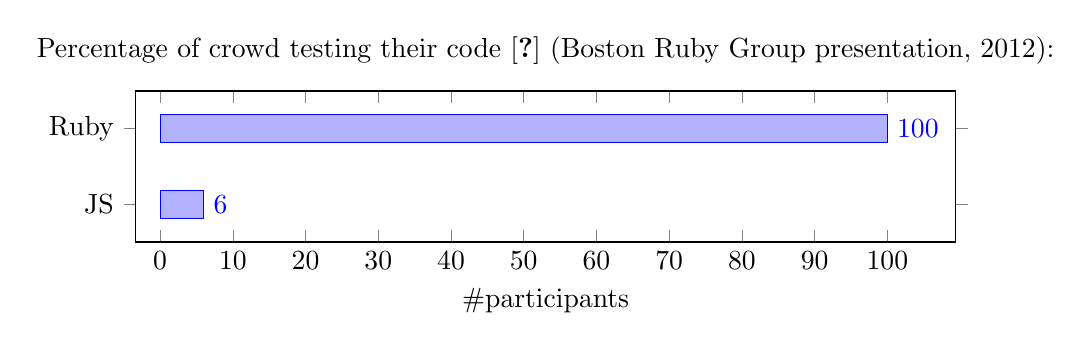
\begin{tikzpicture}
\begin{axis}[
title={Percentage of crowd testing their code \cite{TestingStatistics} (Boston Ruby Group presentation, 2012):},
xbar,
width=12cm, height=3.5cm, enlarge y limits=0.5,
xlabel={\#participants},
symbolic y coords={JS,Ruby},
ytick=data,
nodes near coords, nodes near coords align={horizontal},
]
\addplot coordinates {(6,JS) (100,Ruby)};
\end{axis}
\end{tikzpicture}
\end{center}

The main goal with this thesis was to investigate why \gls{js} and \gls{sml} testing has been performed to such a small extent historically, describe some benefits and practises of doing it, and identifying problems that are yet to be solved. This section contains background and scope, and an overview of the organisation of the thesis.

\subsection{Motivation}
\label{subsec:motivation}

Why testing, you may ask. Jack Franklin, a young \gls{js} blogger from the UK, gives three reasons:

\begin{enumerate}
\item It helps you to plan out your APIs
\item It allows you to refactor with confidence
\item It helps you to discover regression bugs (i.e. when old code breaks because new code has been added)
\end{enumerate}

Writing tests to use a library before actually writing the library puts focus on intended usage, leading to a cleaner API. Being able to change and add code without fear of breaking something greatly accelerates productivity, especially for large applications. \cite{JackFranklin} Without tests, the ability to refactor (see section \ref{subsec:refactor}) is greatly hampered and without refactoring, making changes becomes harder over time, the code becomes harder to understand, the number of bugs increases and more time will be spent debugging \cite[p.~47-49]{Refactoring}. In order to avoid this, code should be tested, preferably as an activity integrated with the rest of the development rather than seen as a separate task. Writing tests first ensures testability, which may also imply adherence to principles such as separation of concerns and single responsibility \cite[p.~35-37]{Clean}.

Tests can serve to prevent people from breaking code and as examples that help new people understand how an application works and how to continue development \cite[questions~31-32]{Edelstam}. Tests can also serve as documentation and monitoring of the code, showing how components fit together and concretising features and bugs. Provided that tests are readable and focus on the behaviour of the code, developers can rely on them to understand the production code that they are unfamiliar with or has not worked with for a long time, and measure progress in terms of implementing acceptance tests. There are also benefits for the product management: awareness of how the product performs on different platforms and software environments is reassuring when communicating with customers \cite[question~38]{Ahnve}.

Figure~\ref{fig:distance} shows an analogy for how testing influences development pace. Developers writing code without tests are like pure sprinter swimmers, they will be fast in the beginning of a project but over time the increasing complexity of the code will force them to go much slower. Developers that writes tests as part of the development process are more like pure distance swimmers, they maintain a sustainable pace. It is arguably slower in the beginning, but productivity does not decrease as drastically over time. The analogy is not perfect -- development pace is typically more dependent on system complexity than swimming speed is on distance, but this on the other hand only serves to further emphasise the point. Testing is a long term investment.

\begin{figure}[ht]
\centering
\includegraphics[width=\textwidth]{pics/distance.png}
\caption{Long distance swimmers are initially slower but have better endurance than sprinters.
A software development project displays similar properties, developing with tests is like training for long distances.
If a project will be large enough to reach break even, testing will pay off.
The graph to the right is not based on any exact data, but merely a sketch based on intuition.
Image courtesy of graph to the left: Paul Newsome at \small \url{www.swimsmooth.com}}
\label{fig:distance}
\end{figure}

Implementations of \gls{js} differ, especially for host objects such as document and XMLHttpRequest whose semantics are not fully defined in the specification but also for native objects that may be missing or behave differently in some implementations because they were not defined in previous specifications. Automated testing can help you discover bugs that appear due to such deviant behaviour in present and future versions. \gls{js} is also particularly important to test due to its dynamic properties \cite{AutomatedTesting} that complicate static analysis (however, there are lint tools, see section~\ref{subsec:refactor}), unwieldy syntax and aberrant object orientation support. \gls{js} is a complex language that requires many work-arounds because of its scoping rules and other unexpected behaviour \cite[appendix A]{GoodParts}. Despite the wide variety of testing frameworks that exists for \gls{js}, it is generally considered that few developers use them and instead rely on manual testing \cite{AutomatedTesting}.

Several implementations of \gls{sml} exist and just as with \gls{js}, there are some differences between them. \gls{sml} has extensive static analysis capabilities and since side effects are relatively rare, the output of functions tends to be predictable, leading to lower complexity in many cases, at the cost of flexibility. \gls{sml} has no built in support for automated testing and there are few testing frameworks available (see section \ref{mltestingframeworks}).

More than 90 \% of today's websites use \gls{js} \cite{BusinessJavascript} and its applications have become increasingly complex \cite[question~23]{Ekelof}. \gls{sml} on the other hand, although not nearly as widespread, is used in critical applications. The potential risk of economic loss associated with untested code being put into production, due to undetected bugs, shortened product lifetime and increased costs in conjunction with further development and maintenance, constitutes the main motivation for this thesis.

\Gls{sml} is a functional language just like \gls{js}, but is not implemented in browsers and has a static type system, lack of (prototype-based) object orientation support, and limited support for mutation. Because of this, \gls{sml} is typically used more in education, back-end logic and algorithm design than for web application front-ends. \Gls{sml} is well suited for formal verification, which in theory is excellent, but practical aspects such as how difficult formal verification is to do, how much benefits there are for maintainability, modularity and code design, and the time and resources required to do it need to be considered. In which scenarios is formal verification feasible? How does it affect productivity and the ability to get quick and frequent feedback whether the program is still correct? Even though testing can seldom provide the same guarantees as formal verification regarding correctness, there are many scenarios in which it is more cost effective and makes life easier for the developer. The two can of course also be used in parallel. See section \ref{subsec:formalverification} for more on formal verification.

Unit testing is particularly powerful when in combination with integration tests in a \gls{ci} build with \gls{autodeploy}.
This enables you to harness the power of \gls{ci}, avoiding errors otherwise easily introduced as changes propagate and affect other parts of the system in an unexpected way. The integration tests will make developers aware if they are breaking previous functionality, when changing parts of the system that the \gls{js} depends upon.

This paves the way for test-driven development, which brings benefits in terms of the design becoming more refined, and increased maintainability. To achieve these gains from testing, the tests themselves need to be of high quality: they should be maintainable, fast and test the right thing. How to achieve this is an important part of this thesis, which is discussed in section~\ref{subsec:stateofevents}.

\subsection{Background to Project}
\label{mltestingframeworks}

This thesis was written at Valtech AB, an IT consulting company based in Stockholm, with 185 employees (2013) specialised in digital strategy and full stack web and mobile development. The company has an interest in techniques for testing \gls{js}, but the subject of this thesis was left to the author to decide.

The first known \gls{js} testing framework JsUnit\footnote{\url{https://github.com/pivotal/jsunit}} was created in 2001 by Edward Hieatt \cite{GoingFaster} and since then several other test framework has appeared such as the testing framework for jQuery: QUnit\footnote{\url{http://qunitjs.com/}}, and JsUnits sequel Jasmine\footnote{\url{http://pivotal.github.com/jasmine/}}. There are also tools for mocking such as Sinon.JS\footnote{\url{http://sinonjs.org/}} (see section~\ref{subsec:mocking}). It seems as if the knowledge of how to get started smoothly, how to make the tests stable and time efficient, and what to test, is rare. Setting up the structure needed to write tests is a threshold that most \gls{js} programmers do not overcome \cite{TestingStatistics} and thus, they lose the benefits, both short and long term, otherwise provided by testing.

There is only one production quality testing framework available for \gls{sml}, namely QCheck\footnote{\url{https://github.com/league/qcheck}}. A few other frameworks exist but have not gained any traction and are relatively small, typically less than a year old and not under active development. The recent increase in the number of testing frameworks could be a consequence of developers being more willing to share their work as open source, an increased use of \gls{sml} testing in education (see section~\ref{subsec:tddmooc}), or an indication that testing in general has been increasingly popular over the last couple of years, as can be seen in the \gls{js} community \cite[question~1]{Edelstam}. An exhaustive list of the other \gls{sml} testing frameworks and a short discussion about their differences can be found in the Appendix.

Material on how to test \gls{sml} properly is hard to come by. Similarly, in guides on how to use different \gls{js} testing frameworks, examples are often decoupled from the typical use of \gls{js} -- the Web -- which is a problem \cite[question~3]{Ekelof} although it has become better compared to a couple of years ago \cite[question~27]{Ahnve}. Examples tend to illustrate merely testing of functions without side effects and dependencies. Under these circumstances, the testing is trivial and most \gls{js} programmers would certainly be able to put up a test environment for such simple code.

Examples are useful when learning idiomatic ways of solving problems. Code tends to end up being more complicated than examples you read because it is hard to come up with useful abstractions that make sense. Those who write examples to illustrate a concept always have to find a tradeoff between simplicity, generality and usefulness, and tend to go for simplicity \cite[questions~56-57]{Edelstam}. This can for example be observed in \cite[p.~13-45]{Refactoring} where the tests and their setup are omitted despite their claimed importance. Combining different concepts may help to achieve code with good separation, that can be tested by simple tests.

In contrast to examples often being simple and seldom providing a full picture, the problem domain of this thesis is to focus on how to test the behaviour of \gls{js} that manipulates \gls{dom} elements, fetches data using asynchronous calls, validates forms, communicates through APIs or manipulates the appearance of a web page (see section \ref{sec:jsproblems}). The domain also includes testing of \gls{sml} in general.

\subsection{Scope and Delimitations}

The scope of this thesis is mainly limited to \emph{automated} testing of \gls{sml} and \emph{client side} \gls{js}. The goal is to investigate what the main problems within these two areas are and how they relate to development tools and practises. What are the testability issues in each respective language? Which considerations need to be made in order to write stable and maintainable tests? How does testing culture affect productivity and quality of software?

The impact of testing frameworks specialised for server side \gls{js} code (node.js) such as vows\footnote{\url{http://vowsjs.org/}} and cucumis\footnote{\url{https://github.com/noblesamurai/cucumis}} was not considered during the project. Testing client side code is not necessarily more important than server side, but in many aspects client side testing is different and sometimes harder. Reasons for choosing \gls{js} and \gls{sml} over other programming languages have already been covered in the introduction.

\gls{js} testing frameworks that are no longer maintained such as JsUnit\footnote{\url{https://github.com/pivotal/jsunit}} and JSpec\footnote{\url{https://github.com/liblime/jspec}} was deliberately left out of consideration. Others were left out because of a smaller user base or lack of unique functionality; among these we find TestSwarm, YUI Yeti and RhinoUnit and the majority of the \gls{sml} testing frameworks (see Appendix). These are useful tools but could not be included due to time limitations.

Manual testing was not covered to any significant extent, since it is outside the scope of test-driven development and automated testing. Naturally, there are many situations where manual testing is required, but in this thesis \emph{testing} typically refers to automated testing.

Since \gls{sml} has a smaller user base than \gls{js}, the majority of the research in this thesis has been focused on \gls{js}. Researching today's limited testing of \gls{js} may be done from different perspectives. There are soft aspects such as:
\begin{itemize}[label={--}]
\item Differences in attitudes towards testing between different communities and professional groups and knowledge about testing among \gls{js} developers (section~\ref{sec:testingculture})
\item How \gls{js} is typically conceived as a language and how it is used (section~\ref{ssubsec:interviewees})
\item Economic viability and risk awareness (section~\ref{subsec:projectrisks})
\end{itemize}

There are also more technical aspects:
\begin{itemize}[label={--}]
\item Testability of \gls{js} code written without tests in mind (section~\ref{sec:testability})
\item Usability of testing tools and frameworks (sections \ref{subsec:jstestdriver} and \ref{subsec:frameworks})
\item Limitations in what can be tested (section \ref{sec:testability})
\item Complexity in setting up a test environment; installing frameworks, configuring build server, exposing functions to testing but not to users in production, etc. (section \ref{sec:testability})
\end{itemize}

An important part of the scope has been to account for how to proceed conveniently with \gls{js} and \gls{sml} testing. The ambition was to cover not only the simplest cases but also the most common and the hardest ones, and to introduce available tools and frameworks. Many tutorials for testing frameworks today tend to focus on the simple cases of testing, possibly because making an impression that the framework is simple to use has been more highly prioritised than covering edge cases of how it can be used that might not be relevant to that many anyway. To provide guidance in how to set up a testing environment and how to write the tests, attention was paid to the varying needs of different kinds of applications. It was also important to describe how to write tests that are as maintainable as the system under test, to minimise maintenance costs and maximise gain.

Rather than proposing best practices for \gls{js} testing, the reader should be made aware that different approaches are useful under different circumstances. This applies both to choice of tools and how to organise the tests.

A full evaluation of the most popular testing and application frameworks is not within the scope of this thesis, but others have done it \cite{JackFranklin}\cite{SebastianPorto}. Popular \gls{js} testing frameworks include assertion frameworks such as Jasmine, qUnit, expect.js and chai, and drivers/test runners such as Mocha, JsTestDriver, Karma and Chutzpah\footnote{\url{http://chutzpah.codeplex.com/}} which may have their own assertion framework built in but are typically easy to integrate with other assertion frameworks using adapters or via built-in support.

\subsection{Organisation of Thesis}

This thesis is about difficulties and experiences with \gls{js} and \gls{sml} testing, and has been organised in favour of readers mainly interested in one of these programming languages. It contains a case study on testability aspects of adding tests to an existing \gls{js} application (section~\ref{sec:testability}), problems specific to \gls{js} and \gls{sml} testing (sections~\ref{sec:jsproblems} and~\ref{sec:smlproblems}), considerations from writing and using a \gls{bdd} framework in \gls{sml} (section~\ref{subsec:describesml}) and implications of testing culture that has been researched through interviews (section~\ref{sec:testingculture}). These sections are preceded by an overview of what others have done in the fields of \gls{js} and \gls{sml} testing (section~\ref{sec:previouswork}), the methods that were used for writing this thesis (section~\ref{sec:methods}) and a technical background that explains some of the concepts that appear in the rest of the thesis (section~\ref{sec:technicalbackground}). The final section is conclusions (section~\ref{sec:conclusions}), including summaries and proposals of future work.

Readers experienced with or uninterested in testing concepts and web application development may skip the technical background (section~\ref{sec:technicalbackground}). Readers interested mainly in \gls{js} testing may skip sections~\ref{subsec:previousworksml}, \ref{sec:smlproblems} and~\ref{subsubsec:whynotsml}. Readers interested mainly in \gls{sml} testing may skip sections~\ref{subsec:previousworkjs}, \ref{subsec:browserautomation}, \ref{sec:testability}, \ref{sec:jsproblems} and~\ref{subsubsec:whynotjs}.

The glossary, which is located before this introduction, contains definitions of abbreviations and technical terms used throughout the text.

\section{Previous Work}
\label{sec:previouswork}

This section contains an overview of what others have done within the fields of \gls{js} and \gls{sml} testing. Particular interest is paid to research -- lists of relevant frameworks and tools can be found in the Appendix.

\subsection{JavaScript Testing}
\label{subsec:previousworkjs}

In 2010, a student at the Swedish royal institute of technology called Jens Neubeck wrote a master thesis about test-driven \gls{js} application development \cite{Neubeck}. In his thesis, he evaluated Crosscheck, HtmlUnit och Selenium, with the conclusion that none of them were mature enough to be used for the considered applications. Today, HtmlUnit and Selenium have evolved and there are new tools available such as PhantomJS, Buster.JS and Karma, so the conclusion might not hold anymore. Tools such as JsTestDriver and Jasmine were not considered and the results were based purely on original work, with no \gls{js} specific academic sources, so it has not been possible to build upon his findings here.

The main source of reference within the field of \gls{js} testing today is \emph{Test-Driven JavaScript Development} \cite{Tddjs} by Christian Johansen, which deals with \gls{js} testing from a \gls{tdd} perspective. Johansen is the creator of Sinon.JS\footnote{\url{http://sinonjs.org/}} and a contributor to a number of testing frameworks hosted in the open source community. The book takes a rather practical approach to \gls{js} testing by explaining many aspects of how \gls{js} works and by including practise exercises. It is not very scientific but makes up for this with its pragmatism and roots in the software industry.

Today blog posts and books about \gls{js} are in abundance and examples can often be found in the documentation of frameworks. When it comes to examples of testing in general, there are several classics to refer to \cite{KentBeck}\cite{TestPatterns}. For examples of \gls{js} testing specifically the alternatives have been scarce historically, but recently a large number of books about \gls{js} testing has been published. \emph{JavaScript Testing, Beginner's Guide} \cite{JSBeginners} is an introductory book about \gls{js} that covers some aspects of testing, \emph{JavaScript Testing with Jasmine} \cite{JasmineBook} covers the Jasmine testing framework in detail, \emph{Behaviour Driven Development with JavaScript} \cite{BDDJS} presents a \gls{bdd} perspective of \gls{js} testing, \emph{JavaScript Unit Testing} \cite{JSUT} looks at the assertions and asynchronous testing capabilities of Jasmine, YUI Test, QUnit and JsTestDriver, \emph{Using Node.js for UI Testing} \cite{UsingNode} covers ways of automating testing of web applications with Zombie.js and Mocha, and \emph{Testable JavaScript} \cite{TestableJS} looks at ways of reducing complexity of \gls{js} code and discusses principles and tools (mainly YUI Test) for \gls{js} testing and maintainability in general. All of these were published this year (2013), except \emph{JavaScript Testing, Beginner's Guide} which was published the same year as Johansen's book, in 2010.

There are many academic articles about testing web applications available, and quite a few of them focus on \gls{js} specifically \cite{AutomatedTesting}\cite{ContractTesting}\cite{AutomatedAcceptance}\cite{Wild}\cite{DOMJavascript}. There is also a lot of material on testing patterns and how to write concise, useful and maintainable tests \cite[part~III]{TestPatterns}\cite[ch.~3-5]{BDDJS}\cite[p.~461-474]{Tddjs}\cite[p.~86-87]{TestableJS}\cite[p.~13-14]{JasmineBook}.

\emph{A Framework for Automated Testing of JavaScript Web Applications} \cite{AutomatedTesting} focus on automatically generating tests to achieve a high degree of code coverage. The problem with this is that the ability to employ test driven development is generally more valuable than high code coverage, due to its effect on the system design (see section~\ref{subsec:coveragecriteria} for further discussion). Automatically generated tests can be harder to maintain and will tend to fail for unintended reasons as the code changes, unless the tests are re-generated.

\emph{Automated Acceptance Testing of JavaScript Web Applications} \cite{AutomatedAcceptance} describes a way to specify intended behaviour of a web application and use a web crawler to verify the expectations. It appears as a promising alternative to using Cucumber in conjunction with Selenium (see section~\ref{subsec:browserautomation}), but more case studies are needed in order to evaluate its usefulness, applicability and scalability. %TODO describe Cucumber

Sebastien Salva and Patrice Laurencot has described how STS automata can be applied to describe asynchronous \gls{js} applications and generate test cases \cite{AutomatedAjax}.

Heidegger et al. cover unit testing of \gls{js} that manipulates the \gls{dom} of a web page using techniques from software transactional memory (STM) to restore test fixtures \cite{DOMJavascript}. Ocariza et al. have investigated frequency of bugs in live web pages and applications \cite{Wild}. These are both aimed at testing client side \gls{js} that runs as part of web sites.

Phillip Heidegger and Peter Thiemann has addressed the issue of type related errors in \gls{js} by introducing JSConTest, a contract framework that enables guided random testing by specifying types and relations of the arguments and return value of functions \cite{ContractTesting}.

\subsection{Standard ML Testing}
\label{subsec:previousworksml}

Except for discussions on how to perform mathematical proofs and equality tests of polymorphic types, there are no books that cover testing of \gls{sml}. The main sources of reference for \gls{sml} are \emph{The Definition of Standard ML} \cite{DefinitionStandardML} which covers the language syntax and semantics, \emph{The Standard ML Basis Manual} \cite{BasisManual} which describes the standard library, \emph{Elements of ML Programming} \cite{ElementsML} which cover the features of \gls{sml} in a more comprehensible fashion, \emph{ML for the Working Programmer} \cite{WorkingProgrammer} which is somewhat outdated but comprehensive, and various lecture notes \cite{ProgSml97}\cite{ProgSmlHarper}\cite{FunctionalML}\cite{NotesSMLNJ}. None of these describe ways of doing automated testing and there seems to be an attitude against testing based on that it can not prove absence of errors in the way formal verification can \cite[p.~16]{ProgSmlHarper}.

Articles on testing of \gls{sml} are hard to find, none cover \gls{sml} testing within a web applications context and most are concerned with formal verification or related to the QuickCheck tool which can be used to generate tests for Haskell code, using \gls{sml} as an intermediate language. However, the ideas of QuickCheck has been directly applied to \gls{sml} in the QCheck testing framework, which is covered in \emph{Random Testing of ML Programs} \cite{RandomML}, a master thesis from 2010. In QCheck, tests are specified in terms of properties rather than generated from the code itself or based on user interaction data. While avoiding the circularity of generating tests based on the code that should be tested, this approach instead suffers from the difficulty of identifying and expressing properties that should hold, and there may be uncertainty in how well the properties are actually tested.


\section{Methods}
\label{sec:methods}

The methods that were used in this thesis comprise situational analysis, interviews, and programming activities in \gls{js} and \gls{sml}. The work of this thesis began with an extensive literature study and an overview of existing technologies and frameworks. Interviews of \gls{js} developers of different background were performed and analysed. There were also hands on evaluation of tools and frameworks, assessment of testability and impact of adding tests to existing projects, and a small testing framework was developed in \gls{sml} and used in a \gls{mooc}.

\subsection{Literature Study}

As mentioned in \nameref{sec:previouswork} (section \ref{sec:previouswork}), several new titles were published while writing this thesis, so the literature study continued to the very end. The books, articles and internet sources served both as reference to complement the interview material and as starting point for many of the experimental testing activities that were carried out (see next subsection).

Since there was an abundance of material on \gls{js} testing, a full review was not viable. For \gls{sml} testing on the other hand, there were virtually no material on \gls{sml} testing available, so any claims had to be based on practical observations and comparisons with formal verification instead. Since many relevant facts and principles hold for more programming languages than just these two, some classical works within the field of testing were included in the study as well.

\subsection{Programming}
\label{subsec:programming}

In order to describe ways of writing tests for \gls{js}, the practical work involved adding tests to an existing \gls{js} application (see section \ref{subsec:asteriods}), performing \gls{tdd} exercises from Test-driven JavaScript Development \cite[part~III]{Tddjs} and doing some small \gls{tdd} projects during the framework evaluation. There were plans to have a workshop field study, where programmers would work in pairs to solve pre-defined problems using \gls{tdd}, but in the end it was decided that it would be too difficult to extract useful data from such an activity.

An \gls{sml} testing framework (see section \ref{subsec:describesml}) was developed and used to solve programming assignments in the Coursera Programming Languages \gls{mooc}. This provided experience of using \gls{tdd} in \gls{sml} (see section~\ref{subsec:tddmooc}), allowed for application of insights from looking at \gls{js} testing to \gls{sml} dito, and made clear which problems within \gls{sml} testing are specific to \gls{sml} and which are not (see section~\ref{sec:smlproblems}).

A thorough evaluation of frameworks for \gls{js} and \gls{sml} was not part of the scope, but since they pose a significant part of how to solve problems with testing, many were involved anyway. The testing frameworks that were part of the practical work are listed in the Appendix. Apart from the \gls{mooc} programming assignments, all code is publicly available on my Github account \emph{emilwall}, together with the \LaTeX~code for this report.

\subsection{Interviews}

The \gls{js} community is undergoing more rapid changes than the \gls{sml} community, so interviews were focused on \gls{js} to obtain up-to-date information about how it is currently used. They were first and foremost qualitative in nature, carried out as semi-structured case studies in order to prioritise insight into the problem domain and gather unique views and common experiences, which might not be picked up in a standardised survey or other efforts to quantitative research methods. The interviews were between 20 and 60 minutes long and were conducted both in person and via Internet video calls.

\subsubsection{Interview Considerations}

The preparations before the interviews included specifying purpose and which subjects to include, select interviewees, preparing questions and adjust the material to fit each interviewee. The chance of finding the true difficulties of \gls{js} testing was expected to increase with open questions. The interviews took place once preliminary results and insights from the literature study could be used as basis for the discussions.

The purpose of the interviews was to investigate attitudes and to get a reality check on ideas that had emerged during previous work. Selecting the interviewees was to a large extent done based on availability, but care was also taken to include people outside of Valtech and to get opinions from people with different background (front-end, back-end, senior, junior, etc.). Unfortunately no female candidate was available, due to the skewed gender representation among \gls{js} developers. There were five interviews and some email conversations, which can all be found in the Appendix.

The interviews were performed in Swedish to allow for a more fluent conversation and minimise risk of misunderstandings. They were transcribed (see Appendix), each question was given a number, and the most relevant parts were translated and included in this report with reference to the question numbers. The interviewees were asked prior to the interviews if it was ok to record the conversation and if they wanted to be anonymous, everyone agreed to be recorded and mentioned by name.

The interviewees received questions beforehand via mail which most of them answered before the interview. This allowed the interviews to focus on the vital parts rather than personal background and opinions about \gls{js}. The questions that were sent out before the interviews were mainly about previous experience with \gls{js} and testing, frameworks, attitudes towards the language, difficulties with testing and opinions and observations on benefits of testing.

\subsubsection{The Interviewees}
\label{ssubsec:interviewees}

\begin{figure}[ht]
\centering
\includegraphics[width=\textwidth]{pics/interviewees.png}
\caption{The interviewees, in order of appearance. Rightmost is Fredrik Wendt, exclusively interviewed by mail. Clearly, there is a skewed gender representation among \gls{js} developers, since all candidates were men.}
\label{fig:interviewees}
\end{figure}

\begin{enumerate}
\item Johannes Edelstam, an experienced Ruby and \gls{js} developer, organiser of the sthlm.js meet-up group, a helping hack, and a former employee of Valtech, now working at Tink. He has a positive attitude towards \gls{js} as a programming language and has extensive experience of test driven development.

\item Patrik Stenmark, a Ruby and \gls{js} developer since 2007. He is also an organiser of a helping hack and a current employee at Valtech. He considers \gls{js} to be inconsistent and weird in some aspects but appreciates the fact that it is available in browsers and has developed large single page applications (SPA) in it.

\item Marcus Ahnve, a senior developer and agile coach who has been in business since 1996 working for IBM, Sun Microsystems and ThoughtWorks, and as CTO for Lecando and WeMind. He is currently working at Valtech. He is an experienced speaker and a founder of Agile Sweden, an annual conference since 2008. He is also experienced with test driven development in Java, Ruby and \gls{js}.

\item Per Rovegård, a developer with a Ph.D. in Software Engineering from Blekinge Institute of Technology. He has worked for Ericsson and is currently a consultant at factor10 where he has spent the last year developing an AngularJS application, with over 3000 tests. He is the author of the programatically speaking blog and has given several talks at conferences and meet-ups, most recently about Angular and \gls{tdd} at sthlm.js on the 2nd of Oct 2013 but the interviews took place in August over Skype.

\item Henrik Ekelöf, a front-end developer who has seven years of professional experience with \gls{js}. He has previously worked as webmaster and web developer at Statistics Sweden and SIX and is now technical consultant at Valtech. I met him in person during my introduction programme in Valtech where he had a session with us about idiomatic \gls{js}, linting and optimisations, but this interview was done over Skype since he works out of town.
\end{enumerate}

\subsubsection{Further Contacts}

As can be seen at the end of the Appendix, there were some additional email conversations. Among those were: Fredrik Wendt, a senior developer and consultant at Squeed specialising in team coaching with coding dojos, \gls{tdd} and agile methodologies. David Waller, teacher at Linnéuniversitetet in a course about Rich Internet Applications with JavaScript. Marcus Bendtsen, teacher at Linköpings Universitet in a course about Web Programming and Interactivity.


\section{Technical Background}
\label{sec:technicalbackground}

This section gives an overview of concepts and tools relevant to understanding this thesis. Readers with significant prior knowledge about web development and \gls{js} testing may skip this section. The topics covered are principles in testing, \gls{tdd}, \gls{bdd}, spikes, refactoring, stubbing, mocking, browser automation and build tools.

\subsection{Principles in Testing}
\label{subsec:testingbasics}

Every developer performs testing in one way or another. Running an application, interacting with it and observing the results is one form of testing. The more time spent on developing the application, the more evident the need for automated tests tends to become (see figure~\ref{fig:distance}), to reduce the amount of manual work and time spent repeating the same procedures.

Automated testing is commonly divided into different categories of tests, that exercise the code in different ways and for different reasons. Unit testing and integration testing is perhaps the most common concepts. Unit testing focuses on testing units (parts) of an application, in isolation from the rest of the application, whereas integration testing is about testing that the units fit together. Sometimes there is an overlap between the concepts, where a unit is relatively large.

Commonly, unit tests are more low level and integration tests are more like user interactions. This does not have to be the case however, unit tests can be written in a business value focused fashion and integration tests may be written before there is even a \gls{gui} to interact with \cite[question~20]{Ahnve}. Thinking in terms of APIs, there is usually a possibility of defining what each part should do, so you can write tests in an outside-in fashion, which reduces the risk of developing something that eventually turns out to be redundant or misdirected (remember, \gls{yagni}) \cite[question~29]{Ahnve}. The downside of this approach is that the code required for such a high level test to pass might be complex, so intermediate tests need to be written. Such a test, that is in a failing state for an extended period of time, is sometimes called a pending test \cite[question~31]{Ahnve}. Pending tests can be useful to guide the development in a clear direction, but the number of pending tests should be kept to a minimum, or else they will become outdated. This can be seen as a consequence of such a test not being timely, thereby breaking the last component of the F.I.R.S.T. principle \cite[p.~132-133]{Clean}.

There are some desirable properties for unit tests, they should be fast, stable and to the point \cite[questions~16-18]{Ahnve}\cite[mail conversation]{Stenmark}\cite[question~12]{Ekelof}. To avoid slow or unstable unit tests and assure that they can be run without an internet connection or in parallel, outer dependencies such as databases, external APIs or libraries commonly have to be abstracted away through stubbing or mocking (see section~\ref{subsec:mocking}). Unit testing suites that are difficult to set up, not frequently brought into a state where all tests pass, or take too long time to run, should be avoided \cite[question~36]{Ahnve}\cite[question~2]{Rovegard}\cite[questions~21-22]{Stenmark}, whereas integration tests are typically slower and require more advanced setup, but they to should be automated and as stable as possible \cite[question~37]{Stenmark}.

There are potentially both good and bad consequences of testing, both from a short and from a long term perspective. A disadvantage is that setting up the test environment and writing the tests take time. If the testing process is not carried out properly, maintaining the tests can cause frustration. The advantages are that if time is spent thinking about and writing tests, the development of production code will require less effort. Testing provides shorter feedback loops, executable documentation and new ways of communicating requirements with customers. The quality and maintainability of the end result is likely to be positively affected and making changes becomes easier, so ideally, the pace of development does not stagnate. The extra time required to set up the test environment and write the actual tests may or may not turn out to pay off, depending on how the application will be used and maintained.

\subsection{Test-Driven Development}
\label{subsec:tdd}

\acrfull{tdd} is ``an iterative development process in which each iteration starts by writing a test that forms a part of the specification we are implementing'' \cite[p.~21]{Tddjs}.

\gls{tdd} shifts focus from implementations to testing, thereby enforcing a thought process of how to translate requirements into tests. When using \gls{tdd}, the most common reason for a bug is because the \gls{tdd} practitioner has moved on prematurely, i.e. not writing enough tests to find a scenario in which the code does not behave as it should or not fully understood the requirements. These kinds of bug would probably persist regardless of if \gls{tdd} is used or not, but the thing to be careful about here is that there is a risk of not putting as much energy into writing flawless production code when using \gls{tdd}, instead relying on iterative improvement and refactoring. % Move or add to conclusions?

A common principle of \gls{tdd}, especially when carried out in a \gls{ci} build, is that the application should frequently be brought to a state where all tests pass \cite[question~2]{Rovegard}. An exception from this rule is pending tests, but as mentioned in section~\ref{subsec:testingbasics}, these should be kept to a minimum.

\subsection{Behaviour-Driven Development}
\label{subsec:bdd}

\acrfull{bdd} is about describing expected behaviour of systems and writing tests from the outside in. It replaces and adds terminology traditionally used within \gls{tdd} and encourages descriptive naming of tests (or \glspl{spec}) that helps readability and to make failure messages more helpful. \cite[questions~17-18]{Ahnve}

An advantage with \gls{bdd} is how it encapsulates ideas about how tests can be organised, for instance through the Given, When, Then (GWT) form (covered in greater detail in section \ref{subsec:frameworks}). In todays \gls{bdd} frameworks there is often a possibility to separate the basic functionality from the special cases by organising \glspl{spec} in nested describes. This can provide an overview of what an application does just by looking at the \gls{spec} output and is commonly seen in open source projects \cite[question~42]{Stenmark}. Providing a context for \glspl{spec} in this way can help to avoid having a single hard-to-read setup for all tests of a class, which is otherwise common in classical \gls{tdd} and testing in general. Having a single setup can be problematic not only for readability reasons, but also because it creates dependencies between tests. A common alternative to the GWT form is nested describe clauses with it-specs as in Jasmine and \gls{bdd} style Mocha. This requires more discipline from the developer because the context has to be covered by the describe text. The classical \gls{bdd} framework RSpec has a \texttt{when} directive that serves as a compromise between the two styles. \cite[question~19]{Ahnve}

Strictly speaking, you do not need a \gls{bdd} framework to perform \gls{bdd}. J. B. Rainsberger, the author of JUnit Recipes: Practical Methods for Programmer Testing, explained how to do \gls{bdd} in jUnit at the XP 2011 conference in Madrid. The key to doing this is to divide the tests based on system behaviour rather than classes. This is the same concept as when writing \glspl{spec} in Cucumber, another Ruby GWT framework, and the same principle applies to \gls{bdd} in \gls{js} (note that Cucumber can also be used to generate acceptance tests for \gls{js}). This is desirable because it helps you to prioritise the parts that truly matters from a business value point of view over implementation details. \cite[question~20]{Ahnve}

\subsection{Spikes in TDD}
\label{subsec:spikes}

Although writing tests first is a recommended approach in most situations, there is a technique for when you need to try something out before you write tests for it, without compromising testability. Dan North, the originator of \gls{bdd}, came up with a name for this technique: spiking \cite{TwitterDanNorth}. The idea is that you create a new branch in your version control repository, and hack away. Add anything you think might solve your problem, don't care about maintainability, testability or anything of the sort. If you find yourself not knowing how to proceed, discard all changes in the branch and start over. As soon as you get an idea about how a solution could look like you switch back to the previous branch and start coding in a test first fashion. \cite[question~59]{Edelstam}

There is an ongoing discussion about whether or not you have to start over after a spike. Liz Keogh, a well known consultant and core member of the \gls{bdd} community, has published posts about the subject in her blog, in which she argues that an experienced developer can benefit from trying things out without tests (spiking) and then stabilising (refactoring and adding tests) once sufficient feedback has been obtained to reduce the uncertainty that led to the need for spiking \cite{Liz1}. She argues that this allows her to get faster feedback and be more agile without compromising the end result in any noticeable way. In another post, she emphasises that this approach is only suitable for developers who are really good at \gls{tdd}, while at the same time claiming that it is more important to be ``able to tidy up the code'' than ``getting it right in the first place'' \cite{Liz2}. It may seem like an elitist point of view and a sacrilege towards \gls{tdd} principles but in the end, whatever makes you most productive and produces the most valuable software has raison d'être.

Counterintuitive it may seem, throwing away a prototype and starting from scratch to test drive the same feature can improve efficiency in the long run. The hard part of coding is not typing, it is learning and problem solving. A spike \emph{should} be short and incomplete, its main purpose is to help you get your mind set on what tests you can write and what the main points in a solution would be. \cite[question~60]{Edelstam}

A similar concept to Spike and Stabilise is to write markup without tests until a feature is needed that could use an API call. Then you write one or several acceptance tests for it, and can start to work with that feature in a \gls{tdd} fashion. \cite[question~30]{Ahnve} %Likheten är inte perfekt, kanske bör tillägga att det inte finns något stabilise-steg i den approachen.
This way of thinking can lead to a useful rationale regarding when to test -- add tests whenever you introduce an external dependency to make sure that dependency is called correctly under certain circumstances, then if that dependency is something that already exists you can just add it, otherwise you can develop it in a test-driven fashion.

Being too religious about testing principles leads to conflicts like ``writing tests take too much time from the real job''. If the tests do not provide enough value for them to be worth the effort then they should be written differently or not at all. There is no value in writing tests just for the sake of it. Thinking about architecture and the end product is usually a good thing, because you need awareness of the bigger picture in order to prioritise correctly and make sure everything fits together in the end. There is the same risk with tests as with other pieces of code, sometimes you are especially proud or fond of a certain test and unwilling to throw it away. In order to avoid that situation it is often better to think ahead and try things out than to immediately spend time writing tests. \cite[question~27]{Edelstam}

\subsection{Refactoring and Lint-like Tools}
\label{subsec:refactor}

Refactoring is ``a change made to the internal structure of software to make it easier to understand and cheaper to modify without changing its observable behaviour'', or the act of applying such changes \cite[p.~46]{Refactoring}. As previously mentioned (section~\ref{subsec:motivation}, \nameref{subsec:motivation}), refactoring prevents program decay and helps to maintain productivity. Just like testing, refactoring is no magic bullet that solves all problems and it is important to know when to do it and when it might not be worth the effort. Suitable situations to refactor are when doing something similar for the third time (a pragmatic approach to the \gls{dry} principle), when it helps to understand a piece of code, when it facilitates addition of a new feature, when searching for a bug and when discussing the code with others, e.g. in code reviews \cite[p.~49-51]{Refactoring}.

There is a serious risk involved in refactoring untested code\cite[p.~17]{Refactoring}, since manually checking that the refactoring does not introduce bugs is time consuming and difficult to do well. However, leaving the code untested means even greater risk of bugs and the refactoring may be necessary in the future anyway, in which case it will be even harder and more error-prone. This problem can be avoided by writing tests first.

A lint-like tool uses static analysis to detect syntax errors, risky programming styles and failure to comply to coding conventions. The use of lint-like tools can be beneficial when refactoring to avoid introducing errors, although it can not fully compensate for lack of tests. There are lint tools available for \gls{js} such as JSLint, JSHint, JavaScript Lint, JSure, the Closure compiler and PHP CodeSniffer. JSLint does provide some help to avoid common programming mistakes, but does not perform flow analysis \cite{JSLint} and type checking as a fully featured compiler would do, rendering proper testing routines the appropriate measure against programming mistakes. There is at least one lint tool available for \gls{sml}, namely SML-Lint\footnote{\url{https://github.com/nrnrnr/SML-Lint}}, but since \gls{sml} is statically typed the need for such a tool is not as great.

Apart from lint-like tools, there are also tools that can be very helpful to see which parts of the code are in most need of refactoring, and to automate certain refactoring actions by facilitating renaming, method extraction, etc. \cite[ch.~5]{Legacy}. Refactoring tools help you identify sections of the code with high cyclomatic complexity, too many methods or with methods doing too many things (or having too many arguments). Relying on metrics such as lines of code is of course not always appropriate due to different coding styles, but at least it provides an overall picture \cite{Kratko}. There is some support for refactoring \gls{js} in IDEs such as Visual Studio (using
JSLint.VS\footnote{\url{http://jslint.codeplex.com/}},
ReSharper\footnote{\url{http://www.jetbrains.com/resharper/}} and/or
CodeRush\footnote{\url{http://www.devexpress.com/Products/CodeRush/}}),
WebStorm IDE\footnote{\url{http://www.jetbrains.com/webstorm/features}} (or
IntelliJ Idea\footnote{\url{http://www.jetbrains.com/editors/javascript_editor.jsp?ide=idea}} using a plugin) and
NetBeans\footnote{\url{https://netbeans.org/kb/docs/ide/javascript-editor.html}}. There are also standalone statistical tools for \gls{js} such as
JSComplexity.org\footnote{\url{https://github.com/philbooth/complexity-report}},
kratko.js\footnote{\url{https://github.com/kangax/kratko.js}} and
jsmeter\footnote{\url{https://code.google.com/p/jsmeter/}} (not to be confused with the
Microsoft Research project\footnote{\url{http://research.microsoft.com/en-us/projects/jsmeter/}}), and general source code analysis software that support \gls{js} such as
Understand\footnote{\url{http://www.scitools.com}},
SonarQube\footnote{\url{http://docs.codehaus.org/display/SONAR/Plugin+Library}} and
Yasca\footnote{\url{http://www.scovetta.com/yasca.html}}.
There seems to be no refactoring tool for \gls{sml} widely available.

\subsection{Mocking and Stubbing}
\label{subsec:mocking}

Mocking and stubbing involves simulation of behaviour of real objects in order to isolate the system under test from external dependencies. This is typically done in order to improve error localisation and execution time, and to avoid unwanted side-effects and dependencies such as communication with databases, across networks or with a file system \cite[ch.~2]{Legacy}. A mock is different from a stub in that it has pre-programmed expectations and built-in behaviour verification \cite[p.~453]{Tddjs}.

\Gls{js} has no notion of interfaces. This makes stubbing and mocking harder, reduces the ability to write tests for an interface before there is an implementation and impedes the ability to write modular or testable code. This is both a reason why testing \gls{js} is hard, and a reason \emph{for} doing it, since testing can compensate for the lack of interfaces by enforcing modularity.

In \gls{js}, tools for stubbing can be superfluous because you are able to manually replace functions with custom anonymous functions, that can have attributes for call assertion purposes. The stubbed functions can be stored in local variables in the tests and restored during teardown. This is what some refer to as VanillaJS \cite[question~53]{Edelstam}. It might come across as manual work that you can avoid by using a stubbing tool, but the benefits include fewer dependencies and sometimes more readable code, as mentioned in section~\ref{LiteralFakes} \cite[questions~54-55]{Edelstam}. However, bear in mind that since \gls{js} has no notion of interfaces, it is easy to make the mistake of using the wrong method name or argument order when stubbing a function manually \cite[p.~471]{Tddjs}.

Typical cases for using a stubbing or mocking framework rather than VanillaJS include when your assertion framework has support for it, as is the case for Jasmine, when you feel the need to do a complex call assertion, mock a large API or state expectations up front as is done with mocks. Bear in mind that overly complex stubbing needs can be a symptom for that the code is in need of refactoring \cite[question~34]{Stenmark}, and strive for consistency by using a single method for stubbing -- mixing VanillaJS with Jasmine spies and Sinon.JS stubs will make the tests harder to understand.

In \gls{sml}, stubbing and mocking can be problematic because of its immutability and lexical scoping. There are situations where replacing a definition with another is technically possible, such as if a dependency is located in another file (then you could import a fake version of the definitions in that file instead) or in the rare case where a mutable reference is used, but in most practical applications there is currently no way of stubbing or mocking in \gls{sml}. Perhaps it would be possible to modify an \gls{sml} implementation to allow it, or do something rash such as allowing tests to temporarily modify the source code containing the \gls{sut}, but that is somewhat far-fetched and error prone.

\subsection{Browser Automation}
\label{subsec:browserautomation}

Repetitive manual navigation of a web site is generally boring and time consuming. There are situations where manual testing is the right thing to do, such as when there is no need for regression testing or the functionality is too complicated to interact with for automated tests to be possible (but then the design should probably be improved). Most of the time, tasks can be automated. There are several tools available for automating a web browser: the popular open source Selenium WebDriver, the versatile but proprietary and windows specific TestComplete and Ranorex, the Ruby library Watir and its .NET counterpart WatiN, and others such as Sahi and Windmill.

Selenium WebDriver is a collection of language specific bindings to drive a browser, which includes an implementation of the W3C WebDriver specification. It is based on Selenium RC, which is a deprecated technology for controlling browsers using a remote control server. A common way of using Selenium WebDriver is for user interface and integration testing, by instantiating a browser specific driver, using it to navigate to a page, interacting with it using element selectors, key events and clicks, and then inspecting the result through assertions. These actions can be performed in common unit testing frameworks in Java, C\nolinebreak\hspace{-.05em}\raisebox{.3ex}{\scriptsize\bf \#}, Ruby and Python through library support that uses the Selenium Webdriver API. \cite{Selenium}\cite{Selenium2}

There is also a Firefox plugin called Selenium IDE, that allows the user to record interactions and generate code for them that can be used to repeat the procedure or as a starting point in tests. In the remaining parts of this thesis, we will mean Selenium WebDriver when we say Selenium, and refer to Selenium IDE by its full name.

\subsection{Build Tools}
\label{subsec:build}

Build programs play an important role in automating testing, and they are often integrated with version control systems. There exists some general build tools that can be used for any programming language, these are often installed on build servers and integrated with version control systems. Examples include Jenkins, which is often configured and controlled through its web interface although it also has a \gls{cli}, and GNU Make, which is typically configured using makefiles and controlled through \gls{cli}. In addition to these, there are also language specific tools: Ruby has Rake, Java has Maven, Gradle and Ant, C\nolinebreak\hspace{-.05em}\raisebox{.3ex}{\scriptsize\bf \#} has MSBuild and NAnt.

Naturally, there are build tools designed specifically for \gls{js} as well, Grunt\footnote{\url{http://gruntjs.com/}} being the most popular, which can be installed as a node.js package, has plugins for common tasks such as lint, testing and minification, and can be invoked through \gls{cli}. \cite[question~52]{Edelstam} Jake and Mimosa are other well known and maintained alternatives. It is also possible to use Rake, Ant or similar. Just as JsTestDriver and Mocha have adapters for Karma and Jasmine (see section~\ref{subsec:frameworks}), Rake has evergreen\footnote{\url{https://github.com/jnicklas/evergreen}} that allows it to run Jasmine unit tests. \cite{BuildTools}\cite[question~6]{Ahnve}

\Gls{sml} has several compilers such as mosmlc and the MLton whole-program optimizer and a large number of interpreters, but they typically have to be manually integrated with other build tools such as GNU Make.


\section{Testability -- Real World Experiences}
\label{sec:testability}

Adding tests for code that was written without testing in mind is challenging \cite[p.~18]{Tddjs}. In this section a case study for doing so in \gls{js} is described, in order to highlight problems and how some of them can be solved. After a short description of how the project was selected and set up, observations regarding the code and the tools used to test it are highlighted, followed by a more general discussion on what to think of when testing an existing application.

\subsection{The Asteroids HTML5 Canvas Game}
\label{subsec:asteriods}

The first step in the case study of adding tests in retrospect was selecting a suitable application. The choice became an HTML5 canvas game, namely asteroids (see figure~\ref{fig:game3}), based on that it combined graphical elements with relatively complex logic and a bit of jQuery, making it a reasonable representative for the typical JavaScript application. Most of the code was reasonably well modularised already from the start and it was easy to get started by simply cloning the repository and opening the supplied HTML file with the canvas element and script locations already defined.

\begin{figure}[ht!]
\centering
\includegraphics[width=1.0\textwidth]{pics/game3.png}
\caption{The asteroids HTML5 canvas game: here the player ship is about to collide with an enemy ship which will destroy them both (unlike what happens when asteroids collide, an example of desirable behaviour to test for)}
\label{fig:game3}
\end{figure}

\subsubsection{Getting Started}
\label{ssubsec:gettingstarted}

The first action was to strip away any redundant files such as iPad specific code and sound files that were not used anyway. This led to a project structure of only game.js, index.html, the licence file, jquery 1.4.1 and a \gls{js} file containing the fonts (used to display score and messages in the game, see figures~\ref{fig:game6} and~\ref{fig:game10}). The next step was to split game.js into separate files in order to test each ``class'' in isolation. This could have been done the other way around, guiding the structure by writing tests first, but it felt natural to work with the source in order to understand it. Refactoring without tests is typically not a good idea \cite[p.~17]{Refactoring}, but it turned out reasonably easy to change the code even without tests as long as care was taken to preserve the order in which the code was executed when moving things to separate files. Since the exercises in \emph{Test-Driven JavaScript Development} \cite{Tddjs} had introduced JsTestDriver, using that with a Jasmine plugin felt like a natural choice at the time, although it involved some issues with syncing the tests in the browser and find the correct versions for the Jasmine adapter to work. The project structure is displayed in figure~\ref{fig:tree}.

\begin{figure}[ht!]
\centering
\includegraphics[width=1.0\textwidth]{pics/tree.png}
\caption{Project structure after splitting \texttt{game.js} into several files and adding JSTD and Jasmine, but before adding any specs}
\label{fig:tree}
\end{figure}

\begin{figure}[H]
\centering
\includegraphics[width=1.0\textwidth]{pics/game6.png}
\caption{After a game over screen has been displayed for one second, the user sees this screen with score of previous game and the ability to start a new game}
\label{fig:game6}
\end{figure}

Later on, tests were added in new directories \texttt{sprites-spec} and \texttt{core-spec}, Sinon.js was added to the \texttt{lib} directory for better stubbing, rendering.js was extracted from main.js to enable more selective execution and a reset.js file was added to the \texttt{core} directory, containing just a single line:

\begin{verbatim}
var asteroids = {}
\end{verbatim}

This line ensured that any old definitions in the asteroids namespace were overwritten before reading the files anew. This should not really be necessary, but was done in order to avoid emptying the cache in between each test run with JsTestDriver. An updated version of the application can be found at \url{https://github.com/emilwall/HTML5-Asteroids}.

\subsubsection{Attempts and Observations}
\label{ssubsec:attemptsandobservations}

Once starting to write tests, the first problems were that some of the code was contained in a jQuery context and that the canvas element was not available in the unit testing environment:

\begin{lstlisting}[language=C++, keywords={function, var, new, if, else, switch, case, break, return, for}]
$(function () {
  var canvas = $("#canvas");
  Game.canvasWidth  = canvas.width();
  Game.canvasHeight = canvas.height();

  var context = canvas[0].getContext("2d");

  ... // Omitted for brevity

  window.requestAnimFrame = (function () {
    return  window.requestAnimationFrame       ||
            window.webkitRequestAnimationFrame ||
            window.mozRequestAnimationFrame    ||
            window.oRequestAnimationFrame      ||
            window.msRequestAnimationFrame     ||
            function (/* function */ callback, /* DOMElement */ element) {
              window.setTimeout(callback, 1000 / 60);
            };
  })();

  var mainLoop = function () {
    context.clearRect(0, 0, Game.canvasWidth, Game.canvasHeight);

    ... // Omitted for brevity

  };

  mainLoop();

  $(window).keydown(function (e) {
    switch (KEY_CODES[e.keyCode]) {
      case 'f': // show framerate
        showFramerate = !showFramerate;
        break;
      case 'p': // pause
        paused = !paused;
        if (!paused) {
          // start up again
          lastFrame = Date.now();
          mainLoop();
        }
        break;
      case 'm': // mute
        SFX.muted = !SFX.muted;
        break;
    }
  });
});
\end{lstlisting}

Efforts to load the contained code using ajax were of no gain, so the solution instead came to involve exposing the contents of the context as a separate class \texttt{rendering.js}, and manually inject the canvas and other dependencies into that class. This required turning local variables such as the 2d-context into attributes of the class, to make them accessible from the original location of the code (the jQuery context). This change introduced a bug that manifested itself only when a feature to draw grid boundaries (see figure~\ref{fig:game8}) was activated. The feature was not important and could have been removed, but solutions were considered anyway for investigation purposes. The bug could be fixed by making a couple of variables in the rendering class globally accessible as attributes, but that would break certain abstractions, possibly making the code harder to maintain. A better solution, which was also eventually chosen, was to move the code for drawing grid boundaries into the rendering class, where it really belonged.

\begin{figure}[ht!]
\centering
\includegraphics[width=1.0\textwidth]{pics/game8.png}
\caption{Draw grid function in action, highlighting cells with sprites}
\label{fig:game8}
\end{figure}

\begin{figure}[ht!]
\centering
\includegraphics[width=1.0\textwidth]{pics/game10.png}
\caption{Game paused while accelerating and shooting towards an enemy ship}
\label{fig:game10}
\end{figure}

The event handling for key-presses could not be extracted since they relied on being executed in the jQuery context for the events to be registered correctly. The event handles had dependencies on local variables in main.js so in order to extract the code into a separate class these local variables would have had to be made global, which would undermine the design by introducing even more global state. Based on this, the event handling code was left without unit tests, leaving it to integration and system testing to detect possible defects such as improper changes to global variables that were used in the event handler.

The major problems however were not of this technical sort, directly related to \gls{js}, but rather had to do with basic testing principles and how the tests were written. The original purpose of the testing was to provide a safety net for further improvement of the game, but it ended up as over-specification because many tests became implementation specific rather than based on what the code should achieve. Other tests, that were more behaviour and feature oriented, instead had issues with insufficient stubbing and cleanup, causing dependencies between tests so that they would fail or pass for the wrong reasons. The insufficient stubbing and cleanup was largely rectified by executing each set of specs in isolation with just the unit under test, without loading any dependencies before stubbing them, and ensuring that any side effects from running the specs affected only a certain namespace, which could then be reset between each test execution. The problem with the test locking the implementation through over-specification remained however.

A notable testability problem was to automate end-to-end testing. The game involved many nondeterministic aspects in how the asteroids moved that would be awkward to control in the tests, so it was decided not to attempt this kind of testing. If it had been attempted, there would probably have been technical challenges in controlling the game, and areas that would have required careful consideration such as what to base the assertions on in the tests. One tool that looked promising was js-imagediff\footnote{\url{https://github.com/HumbleSoftware/js-imagediff}}, which includes a \texttt{toImageDiffEqual} Jasmine matcher for comparing two images as well as utility methods for producing images of an application that uses canvas. It could probably have been used to avoid having to construct fake objects manually for the canvas in unit tests as well. A similar useful module is Resemble.js\footnote{\url{https://github.com/Huddle/Resemble.js}}, that has advanced image comparison features that are useful together with PhantomCSS\footnote{\url{https://github.com/Huddle/PhantomCSS}}.

\subsubsection{Design Considerations}
\label{ssubsection:designconsiderations}

Because there was no documentation available and the application was sufficiently small, \emph{test plans} were written in the form of source code comments about which tests that could be written, in the \gls{spec} files for each class. Arguably, it could have been beneficial to write actual \glspl{spec} but with empty function bodys, but that might would have given an impression that they were passing rather than waiting to be written.

Each function was analysed with respect to its expected behaviour, such as adding something to a data structure or performing a call with a certain argument, and then a short sentence described that behaviour so that it would not be forgotten when writing the actual tests later. Since tests are typically small, one might think that it could be a good idea to write the tests directly instead of taking the detour of writing a comment first, but a comment is inevitably slightly faster to write than a complete test, since it makes up for fewer lines of code and the implementer avoids the risk of getting stuck with details about how to write the test.

\begin{figure}[h]
\centering
\includegraphics[width=0.9\textwidth]{pics/coverage.jpg}
\caption{Tests should be based on desirable behaviour}
\label{fig:coverage}
\end{figure}

Regardless of which tools are used, it is important to remember that testing strategies matter. For instance, coverage should not be a goal in itself, since that will tend toward tests becoming more implementation specific than they would if instead focusing on what the application should do from a high level perspective. When writing tests for the finite state machine (FSM) in the asteroids.Game object of the asteroids application, it took almost 100 lines of test code to achieve clause coverage \cite[p.~106]{AmmannOffutt} for 18 lines of production code (asteroids.Game.FSM.start), see commit 61713c of \url{https://github.com/emilwall/HTML5-Asteroids}. This is not that much, but it didn't provide much value either (except for increased confidence and safer future modification possibilities) as it did not lead to any changes.

Even if attention is paid to what would be most valuable to test, modifying the application to enable these tests will often have an impact on the design. If the code has to be modified in a way that severely breaks the original design and exposes variables that should not be used from any other part of the application, one of two things apply: either you should not test the code in the way you are trying to, or you should rethink the responsibilities of that code. Perhaps it is doing more than one thing, and it is the secondary thing that you feel that you want to test. No wonder then that it feels wrong to expose certain aspects of it, they might not be the primary purpose of that code segment, just an implementation detail. The key-press event handlers mentioned earlier is one example of this -- the mechanism of event handling should probably have been kept separate from the settings and controls logic of the application.

Global state should not be modified by constructors. For instance, when extracting code from main.js into rendering.js, part of that code was involved with initiating the grid, which is shared between all the sprites in the application (through their prototype), which meant that the grid was not defined unless the rendering class had been instantiated. This imposed a required order in which to run the tests and is an example of poor maintainability and design.

The object orientation of the asteroids application provided useful structure and was a rather good fit since it really did contain natural abstractions in the form of objects. An interesting thought is whether the code would have been more testable if it had been written in a functional style. Presumably, there would have been less outer dependencies to locate and isolate in the tests, or less work to instantiate the objects. \cite[question~26]{Ahnve}

\subsubsection{GUI Testing Considered}
\label{subsec:asteroids}

As mentioned in section~\ref{subsec:browserautomation}, Selenium is currently the most popular tool for browser automation. Sometimes it is the only way to test a \gls{js} of an application without rewriting the code \cite[question~43]{Stenmark} (see section~\ref{subsec:openspace} for further discussion) but then tests tend to be brittle and provide little value. In general, since Selenium tests take such time to run they should only cover the most basic functionality in a smoke test fashion \cite[questions~16-17]{Stenmark}\cite[question~21]{Ahnve}. Testing all possible interaction sequences is rarely feasible and should primarily be considered if it can be done fast, such as in a single page application (SPA) where sequences can be tested without reloading the page. \cite[question~44]{Edelstam}

With Selenium IDE (again, see section~\ref{subsec:browserautomation}), there is a possibility of recording a certain interaction and generate code for it. In general, this has has potential of being used to reproduce bugs by letting the user that encountered the bug record the actions that led to it, and communicate with a developer so that proper assertions are added at the end of the sequence. This has some interesting implications, but experience shows that it is hard to do it in practice since it requires the users to be trained in how to use the plugin and to invest extra time whenever an error occurs \cite[questions~42-43]{Edelstam}. In the case of the asteroids application, it would not work at all, since it does not record mouse movements but merely tracks which elements are interacted with and how.

As a consequence of being unable to extract all code from main.js into testable classes, selenium tests were indeed considered as a last resort of testing its behaviour. This would be a reasonably sound usage of selenium because main.js is basically the most top level part of the application and as such can be more or less directly tested with decent coverage, provided the issues with non-determinism would somehow be dealt with. Selenium just recently included the most basic support for testing canvas elements \cite[p.~165-166]{Selenium2}. However, by the time this was considered there was no time for more experimental work with the application.

Using Mocha with Zombie.js (or Phantom.js) as described in \emph{Using Node.js for UI Testing} \cite{UsingNode} was also considered, but deemed as infeasible because that would require more fine grained control over the interaction with the canvas element than what is possible with these tools.

\subsection{Tool Issues}

Selecting which tools and frameworks to use usually has to be done fast and then you have to live with the decision. The decision is nevertheless important, regardless of whether a project has just started or if it is under a maintenance phase. Tools facilitates testing, so that people are not so deterred by the initial effort required to get started. There are many examples of frameworks and tools, such as Yeoman and Brunch, that can help you in quickly getting started with a project, and structure it so that testing becomes easier \cite[questions~11]{Edelstam}. In this subsection we will mainly discuss tools used to write and run the actual tests, and highlight some issues that you might want to be aware of.

\subsubsection{JsTestDriver Evaluation}
\label{subsec:jstestdriver}

When setting up JsTestDriver\footnote{\url{https://code.google.com/p/js-test-driver/}} (JSTD) with the Jasmine adapter there are pitfalls in which version you're using. At the time of writing, the latest version of the Jasmine JSTD adapter (1.1) is not compatible with the latest version of Jasmine (1.3.1), so in order to use it you need to find an older version of Jasmine (such as 1.0.1 or 1.1.0) or figure out how to modify the adapter to make it compatible. Moreover, the latest version of JSTD (1.3.5) does not support relative paths to parent folders when referencing script files in jsTestDriver.conf although a few older versions do (such as 1.3.3d), which is a problem if you want to place the test driver separate from the system under test rather than in a parent folder, or if you want to reference another framework such as Jasmine if it is placed in another directory. % Glossary items for JSTD (and maybe Jasmine, Mocha, etc. too?)

One has to be careful when adding code to beforeEach, setUp and similar constructs in testing frameworks. If it fails the result is unpredictable. At least when using Jasmine with JsTestDriver, not all tests fail despite beforeEach causing a failure, and subsequent test runs may produce false negatives. This is likely due to optimisations in the test driver or that the \gls{sut} contains globally defined objects (rather than constructors). game.js contained such a globally defined object and its tests commonly failed unexpectedly after some other test had failed, and continued to do so in subsequent runs even after the failing test has been fixed. Restarting the test driver and emptying the cache in the captured browser temporarily solved the problem, but was time demanding.

When resuming from sleep on a mac the server needs to be stopped and the browsers need to be manually re-captured to the server, or else the driver hangs when trying to run the tests. This is both annoying and time consuming. However, the problem is not present on a windows machine (and it might not be reproducible on all mac machines either). In the interview with Johannes Edelstam, he agreed that this is one example of something that deters people from testing \cite{Edelstam}.

Definitions are not cleared between test runs, meaning that some old definitions from a previous test run can remain and cause tests to pass although they should not because they are referring to objects that no longer exists or that tests can pass the first time they are run but then crash the second time although no change has been made to the code. Some of these problems indicate that the tests are bad, but it is inconvenient that the tool does not give you any indication when these problems occur, especially when there is false positives. This was why reset.js was needed (see section~\ref{ssubsec:gettingstarted}).

If there is a syntax error in a test, JSTD still reports that the tests pass. For example:

\begin{verbatim}
setting runnermode QUIET
...................................
Total 35 tests (Passed: 35; Fails: 0; Errors: 0) (23,00 ms)
  Chrome 27.0.1453.94 Windows: Run 36 tests (Passed: 35; Fails: 0;
Errors 1) (23,00 ms)
    error loading file: /test/sprites-spec/sprite-spec.js:101: Uncaught
SyntaxError: Unexpected token )
\end{verbatim}

As a developer, you might miss the ``error loading file'' message and that not all 36 tests were run, because the first line seems to say that everything went fine. Sometimes Jasmine does not run any test at all when there is a syntax error, but does not report the syntax error either. It is therefore recommended to pay close attention to the terminal output and check that the correct number of tests were run rather than just checking that there were no failures. This is impractical when running the tests in a \gls{ci} build because the build screen would probably display success even if no tests were run. It can be of help to keep a close look on the order in which files are loaded and also to keep the console of a browser open in order to be notified of syntax errors \cite{MikeJansen}.

\subsubsection{PhantomJS}

The increased maturity of tools such as PhantomJS and Mocha can be truly helpful to get a smooth workflow when adding tests to already existing projects \cite[questions~11-12 and 20]{Edelstam}. An important difference between using a headless browser such as PhantomJS to run your tests compared to running them in ordinary browsers, using for instance JsTestDriver, is that a headless browser provides no information about how your code performs on different \gls{js} implementations. Reasons why you might still decide to do so include speed, easier integration with build tools such as Jenkins, and that it yields the same results as long as the tests focus on logic rather than compatibility. \cite[questions~13-15]{Edelstam}

Error reports are useful feedback that tests provide. The quality of these reports vary depending on which testing frameworks you are using and how you write your tests. When using PhantomJS to run tests, some test failures require you to run the tests in a browser in order to get good error reports. \cite[question~12]{Edelstam}

The unit tests for the asteroids application had an average execution time of roughly 1 ms per test, so there was little to gain from using a headless browser. However, it was done anyway for the sake of research, using \url{https://github.com/larrymyers/js-test-driver-phantomjs}. The results were somewhat surprising -- the execution time increased by an average of 32 \% (see table~\ref{tab:testruns}), rather than decreasing as would be expected.

\begin{table}
  \centering
    \begin{tabular}{ c | c c c c c}
    Test run & Safari  &  PhantomJS  &  Firefox  &  Opera  &  Chrome \\ \hline
     1           &  190    &        246         &    472    &     524    &    \textbf{486}   \\
     2           &  \textbf{173}    &        \textbf{223}         &    513    &     541    &    539   \\
     3           &  180    &        233         &    460    &     465    &    492   \\
     4           &  231    &        257         &    \textbf{413}    &     \textbf{459}    &    551   \\
     5           &  177    &        228         &    467    &     554    &    564   \\
     6           &  182    &        262         &    438    &     475    &    493   \\
     7           &  179    &        239         &    452    &     481    &    617   \\
     8           &  175    &        281         &    492    &     541    &    571   \\
     \textbf{avg}  &  \textbf{185.9}  &    \textbf{246.1}    &    \textbf{463.4}  &   \textbf{505.0} &   \textbf{539.1} \\
    \end{tabular}
  \caption{Time in ms to run 287 tests with JsTestDriver in headless and non-headless browsers. Average for PhantomJS was 246 ms, whereas Safari ran the tests in 186 ms on average -- 24 \% faster. The other non-headless browsers required roughly twice as long time as PhantomJS.}
  \label{tab:testruns}
\end{table}

The tests were run on OS X 10.9, using Safari 7.0 (537.71), PhantomJS 1.9.2 (534.34, installed using npm), Firefox 25.0.1, Opera 18.0.1284.63 and Chrome 31.0.1650.63. Nightly builds of Firefox (28.0a1) and Chrome (33.0.1734.0 canary) were also tested, with average runtimes of 718.5 ms (deterioration) and 482.3 ms (improvement), respectively. The tests were run with a single browser captured at a time, because the running times were longer and more unpredictive when capturing several browsers at once.

Since the \gls{js} engine of PhantomJS was somewhat outdated compared to Safari (534.34 versus 537.71) and the tests contained no dom manipulation that would trigger rendering activities in a non-headless browser, the Safari could perform well despite not being headless. Some efforts were made to run the tests in PhantomJS directly to eliminate the overhead of the JsTestDriver integration (using \url{https://github.com/jcarver989/phantom-jasmine}), but either no tests were run or uninformative error messages were given, although the same test fixture worked in Safari (with a negligible difference in execution time compared to running the tests with JsTestDriver).

\subsubsection{Sinon.JS}

Proper stubbing of dependencies can be a daunting task, and is closely connected to mocking and dependency injection. In \gls{js}, dependency injection is harder than in for instance C or Java because of the absence of class interfaces. The sinon.JS framework does make it easier to stub compared to if done manually (which on the other hand is exceptionally simple to do with \gls{js}) but there are still tradeoffs between dedicating many lines of code to stubbing, quite often having to repeat the same code in multiple places, or risk introducing bugs in the tests themselves.

Deficiencies such as these are important to note because they pose potential reasons to why \gls{js} developers don't test their code. If using the tools and frameworks is perceived as cumbersome and demanding, fewer will use them and those who do will consider it worth doing so in fewer cases.

One could argue that \gls{js} is better suited for testing than most other programming languages because of the built in features than often make stubbing frameworks redundant. The object literals can be used to define fake objects and it is easy to manually replace a function with another and then restore it. An advantage with using manually written fakes is that it tends to make the code easier to understand since knowledge about specific frameworks or DSLs (Domain Specific Language) is not required. \cite[questions~20-21]{Edelstam}\label{LiteralFakes}

JsTestDriver is not perfect. When refreshing and clearing the cache of a captured browser, you have to wait for a couple of seconds before running your tests or else the browser will hang and you have to restart the server. This wouldn't be such a problem if it wasn't because definitions from previous test runs remain in the browser between runs. For instance, if a method is stubbed in two different tests but only restored in the one that is run first, the tests will pass the first time they are run but then fail the second time. Realising that this is what has happened is far from trivial so as a beginner you easily get frustrated with these small issues, since you might refresh the browser quite frequently in the process of finding out.

Having spent many hours debugging, I finally decided to do a thorough check that no test depended on another test or part of the application that is not supposed to be tested by a specific test. In short, I wanted to ensure that the tests I'd written were truly unit tests. In order to do this, I created a copy of the application repository, deleted every file in the copy except for one test and the corresponding part of the application. Then I configured a JSTD server with a browser to run only that test, and repeated the process for every test. This method does not guarantee absence of side effects or detecting tests that do not clean up after themselves, but being able to run a test multiple times without failing, in complete isolation with the part of the application that it is supposed to test, at least gives some degree of reassurance that all external dependencies have been stubbed. If any external dependency has been left unstubbed the only way for the test to pass is if the code exercising that dependency is not executed by the test, and if a test does not clean up after itself it is likely to fail the second time it runs although this too depends on how the tests are written.

\subsection{Lessons Learned}

In this subsection, problems that are common to not just the asteroids application and the selected set of tools and frameworks, are highlighted. There are typically ways to work around at least some of these problems.

\subsubsection{General Issues With Adding Tests to an Existing Application}

Writing implementation specific tests is a common phenomena that can stem from poor experience of writing tests, extreme testing ambitions or, perhaps most commonly, poor understanding of the system under test. It means that you write the tests based on details about the implementation that you have in mind rather than basing them on what the system should do from an interface point of view. These kind of tests tend to be hard to understand and usually have to be changed whenever an improvement of the implementation is considered, but are unequivocally hard to avoid.

A large number of tests is not necessarily a good thing either, since it is harder to overview and maintain a large collection of tests. Unless the system inevitably is so complicated that extensive testing is justified, it rarely pays off to strive for 100 \% coverage, since it takes too much time and the scenarios that might cause problems are at risk of being overlooked anyway. \cite[question~28]{Edelstam}

When adding tests to an existing application, it is easy to lose track of what has and what has not been tested. Having access to a functional specification of the application can be of help but it might be unavailable, incomplete or outdated. Then you have to make a specification of your own, in order to be systematic about what tests you write. This can be done top-down by looking at user stories (if there are any), consulting a user experience expert, talking with the product owner and the users (if any) or identify features to test through manual testing. It can also be done bottom-up by looking at the source code that is to be tested and come up with ideas regarding what it appears like all the functions should be doing. The latter is what was done before adding tests to the asteroids application, as was mentioned in section~\ref{ssubsection:designconsiderations}

\gls{tdd} can be applied even on an application that previously has no tests, by writing tests that document any changes you make to the application, and isolates every bug you might find. One should be careful not to break existing functionality, but if that happens then it can be useful to prevent the bug from reappearing by writing a test for it. This is best done before fixing the bug so you can watch the test fail, increasing the chance that the test is correct and ensuring that the same bug is not introduced again without anyone noticing. Writing tests for an application in its existing form before changing it will increase understanding of how it works and reduce risk of breaking existing functionality. However, the awful truth is that sometimes code needs to be refactored in order to make it testable, as was described in section~\ref{ssubsec:attemptsandobservations}.

Traditionally, coverage criteria has been a central concept in software testing and is still today in many organisations. When doing \gls{tdd} however, the need for thinking in terms of coverage is reduced as every small addition of functionality is tested beforehand. The goal is not to test specific implementation details because that will only make the system harder to change. If a certain function feels complex and likely to contain bugs, the recommended way in \gls{tdd} is not to test it more carefully to compensate, but to refactor in small steps and test new components separately, rather than trying to achieve different kinds of graph and logic coverage for the complex function. When adding tests in retrospect it makes more sense to think about coverage, which may be done when the system is starting to feel complete in order to reduce risk of bugs. There are various tools available for ensuring that relevant parts of an application are exercised by tests and it is often relevant to design tests based on edge cases and abnormal use. As a tester, it tends to pays off having the attitude of trying to break stuff instead of just testing the so called happy flow. Different types of coverage criteria can help in formalising this, as described in Introduction to Software Testing by Ammann and Offutt \cite{AmmannOffutt}.

% TODO Add citation for that coverage criteria has been and still is a central concept in software testing
\label{subsec:coveragecriteria}

\subsubsection{Stubbing vs Refactoring}

If refactoring is required in order to make code testable, the architecture likely needs to change. Sometimes introducing a new object or changing how some dependency is handled is all that is needed. The important thing is to not continue in a direction that will cause the codebase to deteriorate over time \cite[question~34]{Stenmark}. If a lot of work goes into mocking dependencies (see section~\ref{subsec:mocking}) then the tests take longer to write, require more maintenance and the need for integration tests increases. The proper remedy is usually not to reduce the isolation of the unit tests but to refactor the architecture so that each unit becomes easier to isolate. \cite[question~42]{Stenmark}

When a function is defined within a constructor it is hard to stub it unless you have an object created by the constructor available. In some cases you do not have that because the \gls{sut} creates an instance by itself and then you are (as far as I know) out of options except for stubbing the entire constructor, which produces a lot of code in the tests, or changing the \gls{sut} to increase testability, for instance by having the instance passed as an argument or defining the functions that you need to stub on the prototype of the constructor instead of in the constructor. Often it is possible to increase testability without negative impacts on readability, performance, etc. of the \gls{sut}, but not always. Regardless, this requires a skilled programmer and effort is spent on achieving testability rather than implementing functionality which may feel unsatisfactory.

Sometimes it can be hard to know whether or not to stub library functions, such as those supplied by jQuery that have no side-effects, or if you should trust that they behave as expected and steer the control flow via their input and the global state instead. The same applies to simple functions you have written yourself that you think are free of bugs. Not stubbing external dependencies leads to fewer lines of test setup and teardown code and usually better test coverage but can also impose a danger of the unit tests becoming more brittle and similar to integration tests. Apart from the technical considerations of how decisions regarding stubbing affects how the test works, there are readability benefits in reducing the number of test setup code lines on one hand and making the test context explicit on the other.

When an application is tightly coupled, stubbing easily becomes a daunting task. What you end up with is deciding whether you should compromise the unit tests by keeping the level of stubbing to a minimum, refactor the code to reduce the amount of calls that needs to be stubbed, or engage in voluminous stubbing. The first alternative bodes for unstable tests that might fail or cause other tests to fail for the wrong reasons. Refactoring might introduce new bugs and should only be considered if it significantly improves the design. Stubbing all dependencies might result in an impractical amount of setup code with complicated testing. The only way to avoid this dilemma is \gls{tdd}, which would enable more aggressive refactoring. This tradeoff had to be made when tests for classes that depended on the Sprite class were written. The Ship class used Sprite both for its ``exhaust'' attribute and for its prototype. A common principle is that constructors should not modify or depend upon global state. Luckily, the Sprite constructor adhered to that principle, so in this case not stubbing the Sprite class before parsing the Ship class was acceptable. However, all calls to methods defined in Sprite were stubbed, since they were tested separately.

Sometimes during the process of adding tests to the asteroids application, the tests accidentally ended up with incomplete stubbing. Detecting this sort of test smell was non-trivial, because there was no automated way of ensuring that a test accessed only a certain part of the application. It was not an option to manually organise the files to ensure that just the appropriated code was loaded, since attempting to stub a function which is not defined produces an exception in sinon.JS, in order to prevent you from making typing errors. This could be circumvented by manual stubbing, but abandoning sinon.JS for that reason felt inconvenient, especially considering that the separation from the code that should not be executed by the tests had to be done manually, so instead I opted towards simply being more careful not to miss any calls that should be stubbed. A semi-automated approach might be possible, using coverage reports to inspect that only the desired code is executed when a certain test is run, but that was not investigated.

As a programmer you have to be very methodical, principled and meticulous not to miss some detail and write an accidental integration test. Such mistakes leave you with misleading failure result messages and sometimes the tests fail because of the order in which they are executed or similar, rather than because of an actual bug in the \gls{sut}.

\subsubsection{Deciding When and What to Test}

When deciding what to test, it pays off to focus on parts that are central to how the application is perceived, for instance pure logic and calculations might be more important than pictures and graphs. An error that propagates through the entire application is more serious than if a single picture is not displayed properly. If a test turns out to be difficult to write or frequently needs to be replaced by another test, it is usually worth considering not testing that part at all. \cite[questions~9-10]{Edelstam}

Testing is especially important for large applications. It is extra valuable when new functionality is added because it helps to verify that old functionality is not broken and that the new code is structured appropriately \cite[questions~6-7]{Stenmark}. You should then focus on testing behaviour rather than appearance and implementation details \cite[question~10]{Edelstam}. Rather than testing that a certain class inherits from another, test that the methods of that class behaves as one would expect. Whether or not that is dependent on the inheritance patterns is mainly relevant for stubbing considerations -- you may want to replace the prototype of an object in tests so that you can check that there are no unexpected dependencies.

Something that came up during the interview with Edelstam was that when a certain section of code feels hard to test, it is likely that any test you write will become rather brittle as the code changes in the future. The proposed solution was to avoid testing it unless the code can be refactored so that testing becomes easier \cite[question~30]{Edelstam}. When writing the tests for the asteroids application, it was deliberately decided to write tests even when it felt hard, or when it felt like it provided little value, to see whether this made the application harder to test or modify later.

Because unit tests are typically fast, it is common practice to prioritise decent coverage and corner cases in the unit tests rather than in integration, UI, e2e (end to end) and other types of tests. When tests can be executed fast, they are more useful when changes are made to the code. This is especially important when someone other than the person who wrote the code is making the changes, or when some time has passed since the code was written. \cite[questions~22-24]{Stenmark} % Glossary for e2e?

Naturally, the more important a certain functionality is in relation to business value, the more effort should be put into e2e and similar tests related to it. Inherently complex parts of the code and code that is likely to change should be tested by unit tests to allow for refactoring and increase chance of discovering bugs, whereas simple code that is not expected to change can be tested manually. However, it is typically hard to know beforehand if the code you are writing is subject to change, so a compromise by writing a few simple tests for that code may pay off. \cite[questions~28-29 and 33]{Stenmark}

In the end, when deciding what tests to write, one of the most important things are to make sure that the tests are meaningful. They should in some way be connected to the problem that the system solves and describe something that matters rather than just testing methods for the sake of it. \cite[questions~17-18]{Ahnve}

\subsubsection{A Related Experience}
\label{subsec:openspace}

During a talk at a meet-up on python APIs (2013-05-22 at Tictail's office, an e-commerce startup based in Stockholm), the speaker mentioned that their application depended heavily on \gls{js}. It turned out that they had done some testing efforts but without any lasting results. During the open space after the talks, testing became a discussion subject in a group consisting of one of the developers of the application, among others. The developer explained that they had been unable to unit test their \gls{js} because the logic was too tightly coupled with the \gls{gui}. This meant that the only observable output that they could possibly test was the appearance of the web page, via Selenium tests. He sought reassurance that they had done the right thing when deciding not to base their testing on Selenium, which he considered unstable (tests failing for the wrong reasons) and slow. He also sought advice regarding how they should have proceeded.

The participants in the discussion were in agreement that testing appearance is the wrong way to go and that tests need to be fast and reliable. The experience with testing frameworks seemed to vary, some had used Jasmine and appreciated its \gls{bdd} approach and at least one had used Karma (under its former name Testacular). The idea that general \gls{js} frameworks such as AngularJS could help in making code testable and incorporating tests as a natural part of the development was shared and appreciated. The consensus seemed to be that in general, testing \gls{js} is good if done right, but also difficult.


\section{Problems in JavaScript Testing}
\label{sec:jsproblems}

Considering the variety of available frameworks, one may be deceived into thinking that people do not test their \gls{js} because they are lazy or uninformed. However, there are respectable obstacles for \gls{tdd} of \gls{js}, both in the process of fitting testing frameworks into your application and in writing testable \gls{js}. This section covers how to test asynchronous events, \gls{dom} manipulation, form validation, the \gls{gui} and APIs, in \gls{js}.

\subsection{Asynchronous Events}
\label{subsec:asynchronous}

\gls{js} is often loaded asynchronously in browsers to improve performance in page loads and minimise interference with the display of the page. Another asynchronous aspect of \gls{js} are events such as AJAX calls and timer dependent functions. Testing asynchronous events can be hard because execution order is not predetermined, so the number of possible states can be very large, thus demanding many convoluted tests to cover all the relevant cases. It can also be hard to know if the asynchronous code has finished execution or not, leading to assertions being executed at the wrong time.

Two basic approaches to testing asynchronous code are to force the execution into a certain path by faking the asynchrony, and to set up waiting conditions for when assertions should be executed. When forcing the execution path, the code is not executed asynchronously but you can test different scenarios and thereby get a good feel of how the code will behave when run asynchronously. When using waiting conditions, timeouts need to be set for when tests should fail if waiting conditions are not met.

Most unit testing frameworks supports asynchronous testing through waiting conditions or similar constructs, with some differences in syntax and how it works. There are guides for how to use these aspects of the frameworks in both literature and blogs, for many major testing frameworks: Jasmine \cite[p.~35]{JasmineBook}\cite[p.~45-49]{JSUT}, Mocha \cite[p.~59-65]{UsingNode}, YUI test (only explicit wait) \cite[p.~78-79]{JSUT} and qUnit \cite[p.~114-116]{JSUT}. There are also a large number of relevant blog posts for asynchronous \gls{js} testing
\footnote{\url{http://lostechies.com/derickbailey/2012/08/18/jasmine-async-making-asynchronous-testing-with-jasmine-suck-less/}}
\footnote{\url{http://lostechies.com/derickbailey/2012/08/17/asynchronous-unit-tests-with-mocha-promises-and-winjs/}}
\footnote{\url{http://www.htmlgoodies.com/beyond/javascript/test-asynchronous-methods-using-the-jasmine-runs-and-waitfor-methods.html\#fbid=eILq_Eu-N_I}}
\footnote{\url{http://www.htmlgoodies.com/beyond/javascript/how-mocha-makes-testing-asynchronous-javascript-processes-fun.html}}
\footnote{\url{http://blog.caplin.com/2012/01/17/testing-asynchronous-javascript-with-jasmine/}}. %these should be in the bibliography and perhaps mentioned under previous work

\emph{Test-driven JavaScript Development} claims that JsTestDriver has no built in support for asynchronous testing so it proposes other approaches \cite[p.~247-387]{Tddjs}, but the support was added to the development branch the same year (2010) and is now part of the release: \emph{JavaScript Unit Testing} provides an example of using the \texttt{AsyncTestCase} object in JsTestDriver to extend test methods with a queue parameter \cite[p.~143-145]{JSUT}.

A common concern is that the large number of possible combinations in which asynchronous code can be executed leads to a combinatorial explosion. This is true, but it is also true that if there are few dependencies between the asynchronous code and if they do not share resources, the risk for data races and similar issues is smaller. Therefore, an important part in achieving testability of asynchronous code is to strive for such designs.

The issue of testing asynchronous code is not unique to \gls{js}, e.g. Erlang message passing is also asynchronous, and has been used in systems with high demands on stability. One may ask how Erlang programmers test their code, but answering that question and relating the answers to testing of \gls{js} is such a large project that it could make up for an interesting study of its own. Many other languages with support for multiple threads or processes arguably have this issue as well.


\subsection{DOM Manipulation}

A key to successful testing of \gls{js} with \gls{dom} manipulation is to separate the logic from the \gls{dom} manipulation as much as possible. One technique that was presented at the XP conference in Trondheim 2010\footnote{Agile Processes in Software Engineering and Extreme Programming 11th International Conference, XP 2010, Trondheim, Norway, June 1-4, 2010, Proceedings} was to define a view layer of jQuery-related and similar code, and update the view as a separate task in the business logic. This allows for test driven development to be carried out much more effortlessly than if the logic is tightly coupled with the \gls{dom} manipulation. \cite[question~4]{Ahnve} %Put in bibliography

You can test your \gls{dom} manipulating code if you really need to, but be aware that there are many implementation differences depending on which browser or testing environment the tests are run in (on the other hand, this is one of the reasons why you might WANT to test the \gls{dom} manipulations) and that it can be hard to keep test fixtures up to date.

There are free cloud-based tools such as TestSwarm that are designed to help you with running the tests in many different browsers, or you can do it manually using JsTestDriver, which also has built in support for setting up \gls{testfixture} \glspl{dom}. This is covered in \emph{Test-driven JavaScript Development}, which also shows how it can help to identify reusable components in views \gls{dom} \cite[p.~389-435]{Tddjs}. The qUnit testing framework is also well suited for testing \gls{dom} manipulation\footnote{\url{http://qunitjs.com/intro/\#testing-the-dom-manipulation}}. There are more techniques for unit testing \gls{dom} manipulation but they are not covered here due to space and time limitations.

Aside from unit testing, you can use different Selenium drivers to check almost anything, but beware that such tests easily become slow so even for a medium sized application you might end up being unable to run the tests more than a couple of times per day. Tests can be made to run faster if they run in a headless browser such as PhantomJS, which has support both for Selenium, or by using more specialised tools such as CasperJS which can produce very similar results as Selenium but executes faster and is easily controlled using \gls{js} \cite[p.~142-146]{TestableJS}.

\subsection{Form Validation}

A common case of user interface testing is form validation. A \gls{tdd} extremist might think that you should test that the form exists, has a working submit button and other boilerplate things, but that is mostly irrelevant unless the form is written in a way that is unique or new in some way. A typical approach would rather be to write the code for the form and then add a test that searches for a non-existing validation. The difficult part here is to strike a balance and be alert to when the code is getting so complicated that it is time to start testing, and to avoid writing tests when they are in the way and provide little value. \cite[questions~24-25]{Edelstam}

Validation of forms is commonly done both server and client side so that users do not have to wait for requests to be sent to and returned from a server in order to validate input, while maintaining the security that server side validation offers. Preferably, these validations are automatically kept in sync by frameworks and ideally it should be enough to test the server side validation, but that is sometimes just as hard and to be sure you should test both.

Tools for client side form validation include Parsley\footnote{\url{http://parsleyjs.org}, \url{https://github.com/guillaumepotier/Parsley.js}}, validate.js \footnote{\url{http://rickharrison.github.io/validate.js/}, \url{https://github.com/rickharrison/validate.js}} and the jQuery Validation Plugin \footnote{\url{http://jqueryvalidation.org}, \url{https://github.com/jzaefferer/jquery-validation}}. It is also possible to use the built in support in HTML5 (which however will not work in old browsers) or implement custom validation that is called with onsubmit or onblur. However, form validations should not just have to be implemented, they should be tested too.

You typically need to test for both type I and type II errors (false positives and false negatives). If forms are prevented from being submitted because of an error in the validation (type I error), the number of successful conversions (website goal achievements) is likely to decrease. Allowing invalid forms to be submitted (type II error) can either cause prolonged feedback for the user, loss of form data so the user has to re-type and loss of context due to loading an error page resulting in decreased conversion rates or, if the validation fails at the server side too, security issues.

A real life example of a false positive in form validation is that a personal number is interpreted wrongly, producing an error message falsely claiming that that the applicant is not old enough. In such cases, most people might choose another provider of the service. Proper testing of the form validation could detect this at an earlier stage, thereby avoiding loss of potential customers. \cite{TwitterMe}

A similar bug was observed this year on a scandinavian internet bank. When entering the personal ID it got copied to the password field, and when entering the password it got copied to the personal ID field, so you had to use a cellphone identification service in order to log in. Such a thing would not happen if the bank had automated cross browser testing of the forms. \cite[question~38]{Ahnve}

So how can form validation be tested? Selenium is one option, to enter form data and submit and then check that the proper validation error was printed out at the right location. A benefit with this approach is that a user interaction can be closely imitated. A problem is that if you have many validations that you need to test, these tests tend to take a lot of time.

Depending on which framework you're using, you might have different options for testing. Just testing the validation rules without involving the forms at all can be of great value, e.g. if you are specifying the validation using regular expressions, hopefully you can expose these for isolated testing so that you can avoid testing all the validation in slow integration tests. This will not detect runtime errors or similar for the actual validation, but for complex validation such as testing which strings match a certain regular expression, you are typically better off with fast unit tests, which can be complemented by a smaller number of smoke tests for the integration.

A common case is that you are using another programming language than \gls{js} for the back-end, and you specify the validation rules in that language and let for instance a jQuery plugin generate validations for the front-end. Here you can hopefully put regular expressions and the like as publicly available variables and access them directly in tests, whereas the plugin will have to be tested separately, using perhaps a single test that just checks for existence of validation.

\subsection{GUI Testing}

A \acrfull{gui} is usually the top layer of an application and is therefore a common target for system testing. It can consist of many components and typically provides a large number of possible interactions, which is why \gls{gui} testing is important, but also part of why it can be a time consuming activity both in terms of preparing and executing tests.

\subsubsection{Application Differences}

A rather common opinion is that you should avoid automatic testing of an application's visual components. However, the value provided by \gls{gui} tests depends on how important the \gls{gui} is for the application. In web applications, the \gls{gui} and sequences in it are commonly more complex than the logic underneath, so testing the \gls{gui} makes more sense for such applications than for typical desktop or financial applications where backend logic tend to be more important. \cite[question~21]{Ahnve}

Before deciding on whether you want to do automated \gls{gui} testing or not, think carefully about how important the \gls{gui} and its cross browser compatibility is to you. If you feel that the exact appearance is irrelevant, then there is little sense in doing it. If you on the other hand feel that it would be valuable but have concerns about the technical aspects of it, you should not dismiss it too easily.

The problems that some people experience with testing front end interfaces sometimes have to do with poor modularity. For instance, the presentation layer should not be responsible for calling large APIs. In order to improve the modularity, tools such as RequireJS can be used to handle dependencies but if each part of the application has too many or large dependencies, mocking still becomes a daunting task. Typically, these kinds of problems can be solved by introducing new layers of logic and services that separate responsibilities and allows for much cleaner tests. \cite[question~23]{Edelstam}

\subsubsection{Regression Testing of GUI}

\gls{gui} testing should not be confused with integration testing. Testing graphical elements in tests that depend on system integration are hard to maintain and can fail for too many reasons. Instead of executing a sequence before making assertions about graphical components, you may benefit from keeping assertions simple in an integration test. The \gls{gui} testing can then be performed in a unit testing fashion as a separate activity, by creating a \gls{testfixture} that mimics the state of the application the way it looks after a certain sequence has finished.

This approach has a fairly obvious risk. What if a \gls{testfixture} fails to simulate an application state properly? You could detect this by comparing the application state with the corresponding \gls{testfixture} in an integration test, deliberately introducing dependencies between tests. It might also be hard to construct such a \gls{testfixture} to begin with, or you may feel that it introduces too much maintainability burden to have a \gls{testfixture} that needs to be updated every time a relevant change occurs, in which case you have little choice but to either write bad \gls{gui} tests or skip writing them altogether.

Just as you might decide for or against implementing rounded corners that work in old browsers, based on the number of clients actually using such browsers and the maintenance cost of implementing it for every picture of a site, there is always a tradeoff regarding whether or not to test such graphical elements with automated regression tests or not. In the end, all that matters is cost versus gain, no matter what personal beliefs and preferences might be involved from the product owner or developers' personal points of view. \cite[questions~40-44]{Ahnve}

\subsubsection{Automation of GUI Testing}

Manually testing a web page with all the targeted combination of browsers, versions and system platforms is usually not a viable option \cite{TestSwarm} so multi-platform automated testing is required. This is true in general for web application testing, but also holds for \gls{gui} testing in particular, regardless of whether the \gls{sut} is a web application or not. Since the appearance of a \gls{gui} can depend on factors such as configuration of hardware, operating system, version of third party software, etc., and because of the many possible sequences of interactions to test, it is rarely feasible to test all combinations and unless the testing is automated on multiple platforms, you will be unable to test even a small fraction of them.

\gls{gui} testing can be done in a semi-automated fashion. There are ways of producing snapshots of how websites look in different browsers and you should be able to have a program compare such snapshots to spot differences with previous versions, that can be reviewed by a human. This would reduce the need for manual testing of the \gls{gui}, since you get a good indication of which parts have changed. % http://piwik.org/blog/2013/10/our-latest-improvement-to-qa-screenshot-testing/

Apart from writing tests in code using for instance \gls{tdd}, there are techniques for automatically generating tests using crawlers or artificial intelligence. These techniques will by nature have more focus on coverage and detecting runtime errors than to simulate the behaviour and expectations of users. There has been quite a lot of research in this area \cite{AutomatedTesting}\cite{AutomatedAcceptance}\cite{AutomatedAjax}.

Another technique is capture-replay, which is based on the concept that a user interacts with the \gls{sut} and records the actions. Selenium IDE provides this possibility, and there are other tools as well that can do this both for web and desktop applications.

A more modern approach is model based (FSM) \gls{gui} testing, where graphs are used to represent how the \gls{sut} can be interacted with and which states should be possible to reach. From such a graph, test cases can be generated.

\subsection{External and Internal APIs}

Tests involving an external API need to be kept up to date and in order to do so, integration tests are needed. In essence, problems of maintaining external APIs hold for any external dependencies that you do not have full control over. Testing towards a true implementation is problematic because it takes too long, manipulates data that should not be touched or because the API owner does not accept large amounts of traffic or requires payment for it. Then you typically run the integration tests less often and stick to mocked APIs with fake objects to compensate. \cite[questions~19-20]{Stenmark}

Testing internal APIs (that exists within the same application or organisation) differs from testing calls to an external API in that the latter are often well documented, versioned and rarely changes. When using an external API, the main concerns are making sure that the correct version is used and that the API is called in a correct way with respect to that version. An internal API on the other hand may change frequently which means that the fake objects representing requests and responses of the API in other tests need to change as well. Internal APIs need to be tested because endpoints frequently change and may be used in several places. It is then important to have integration tests that can detect when the fakes need to change. \cite[questions~34,~36]{Edelstam}

Introducing versioning for internal APIs is not always feasible due to the organisational overhead it introduces, for at least two reasons. There can be difficulties in keeping track of the different versions and there can be a risk of hampering development since the parts that use the API are dependent on new versions of the API to be released before they can be updated. However, there exists testing techniques that can be employed regardless if versioning is in place or not. One such technique is to write tests for what characterises an object that the API serves as an interface for, to be able to determine if an object is a valid response or request. These tests can then be used on both real objects and on the fake objects that are used in other tests, which means that when the API changes the tests can be updated accordingly and then the tests involving the fake will fail. Changing the fakes so that the tests passes will hopefully result in that any incompatibility is discovered since the fakes are used in other parts of the testing suite as well. \cite[question~34]{Edelstam}

Testing an internal API is not the same thing as testing a private method. In \gls{js} there is formally no private methods, only functions not exposed to the current scope, nevertheless methods that are not intended to be called from the outside can be considered private. It is common practise not to test private methods. If a private method contains code that can not be tested through the public API, then that method is probably too complex to be private and its functionality should be moved into somewhere else. Private methods represent implementation details, tests should be focused on behaviour and functionality, not implementation. \cite[questions~62-63]{Edelstam}

\section{Problems in Testing of Standard ML}
\label{sec:smlproblems}

\Gls{sml} and \gls{js} have at least two things in common: they are both functional languages (although JS is perhaps more rarely used as such) and they both have poor testing cultures. This section covers existing frameworks, formal verification, and introduces a new \gls{sml} testing framework that was developed as a part of this thesis, inspired by insights gained from looking at popular \gls{js} testing frameworks. In section~\ref{sec:testability}, we discussed how adding tests to an application written without testing in mind can introduce testability issues. Later in this section (~\ref{subsec:tddmooc}) the challenges of writing tests first is described based on a \gls{tdd} approach to solving \gls{sml} programming exercises in a \gls{mooc}.

\subsection{Current Situation}

The SML/NJ and Moscow ML language implementations\footnote{\url{http://www.smlnj.org/svn.html}}\footnote{\url{https://github.com/kfl/mosml}}, and other \gls{sml} projects, have tests for large portions of the code, but there is no standard way of writing the tests. Each module typically ``reinvents the wheel'' by having its own scripts for testing, that is invoked differently and produces different output. If you search the web for ``Standard ML testing framework'' (with quotes, Nov 2013), you get zero results. Dig deeper, and you'll find QCheck/SML (henceforth referred to as QCheck) and a few small testing framework projects without any large user bases (see Appendix). It seems \gls{sml} testing suffers from lack of motivation or knowledge among developers, or availability of good tools. % footnotes after "other projects"

As a programmer, you should strive to do the simplest thing possible within the confines of given constraints, and to reuse as much as possible provided that any reuse candidates meets demands on quality and adaptability. \Gls{yagni} advocates this and is incorporated in many programmers' ways of thinking. When starting to write tests in a project, the pragmatic approach is to adhere to existing codebase conventions, or, in the absence of such, search the web for a suitable testing framework and use it in the project. Why is it that so many end up writing tests without using an existing testing framework? It seems that \gls{sml} developers prefer writing their own testing framework rather than using an existing one.

As indicated by its 30 ``stars'' on github (Nov 2013), the currently most popular testing framework for \gls{sml} is QCheck. However, it is somewhat cumbersome to use in scenarios where property testing is not the main objective. Some may decide against using it because they want something that is simpler, more suitable for \gls{tdd}, or has a different (e.g. \gls{bdd}) style of defining tests and formulating failure and success reports. Without any production quality framework out there that satisfy these basic needs, it may feel like an easier task to do without a testing framework or write a new one than to familiarise with and adapt to an existing one that might turn out as disappointing anyway. The chance of developers deciding to use a framework relies on well prioritised features, active maintenance and a professional, practical or in other ways appealing presentation and reputation.

There are different driving forces behind testing different languages (such as \gls{js} and \gls{sml}), because of the background and motives of people using them, and because of the diversity of the applications in which they are used. This partially explains why QCheck as the only truly popular testing framework for \gls{sml} is based on generating test cases for properties rather than simple expectations/assertion based testing. The developer behind QCheck is Christopher League, a professor at LIU (Long Island University) Brooklyn, so his academic background in computer science is one of the answers. It could be that mathematicians are drawn to the language and are inclined to think in terms of properties and how they can be falsified rather than stating expectations on program state or output.

Another possible reason is that testing for expected output is easy even without the use of a testing framework, whereas QCheck solves problems that are not as easily solved ad hoc. Since \gls{sml} has scripting capabilities, it is relatively easy to write and run tests without a testing framework, compared to doing it in languages that are more verbose and less often used in an interpreted setting, such as Java. Adding a testing framework becomes a bigger deal in \gls{sml} for this reason. Possibly people simply do not find it worth their time to learn testing frameworks just to get readable tests and good failure reports, but instead are content with simply declaring tests as variables that evaluate to true or false, or similar. The consequences of doing this, however, are likely to include more debugging and risk of not noticing when tests fail, or ending up spending a lot of time scrolling through results of the ad hoc tests.

Yet another issue is the methods for distribution. In Node.js installing a package is very easy with the NPM and there is a central place to find popular node modules (\url{https://npmjs.org}). For \gls{sml} there is the SML/NJ Compilation Manager (CM) and Smackage to choose between, and no central repository for modules except for github. Authors of testing frameworks might find it hard to decide which package manager (CM or Smackage) to use, figure out how to use it, or reaching out to users -- which may also find learning how to use a package manager too cumbersome. Reputation, availability, ease of installation and use, and nice presentation may be essential for getting people to use a framework. % Node.js och NPM => glossary eller technical background?

Certain testing frameworks provide a watch capability, that runs tests whenever a change to the \gls{sut} is saved to the file system. In order for this to scale, only relevant tests should be run, or else the benefit of instant feedback is lost. Relevant tests are typically the ones that could be affected by changes in the specific files that have changed, but may also be selected based on speed or past failure rate. The idea is similar to having a build screen for a \gls{ci} build, making not only the tests automated but also the task of running them frequently, and helps ensuring short cycles of writing a failing test, making it pass and refactor.

Mocking and stubbing may not be as important in a functional language like \gls{sml} compared to more imperative languages, since dependencies can often be passed as arguments and functions tend to behave the same way between calls given a certain input. Doing call assertions is as much about architecture as it is about state, and state is mainly kept in which data flows in and out of functions in a functional program, rather than in values of mutable variables as is often the case in imperative programs. However, there are certainly places where it would be appropriate to stub or mock a dependency in a function without having to redesign the function so that the dependency is passed as an argument, and in those cases the lexical scope rules and immutability of \gls{sml} makes it hard to do so. It might be possible to implement a mocking framework that parses the code of a \gls{sut} and produce new bindings that have the desired dependencies and assertion capabilities, but such a framework would have to be quite sophisticated in order to not break the code and is therefore outside of the scope for this thesis. A simpler approach would be to ensure that any dependencies are bound to stub functions before the \gls{sut} is loaded, so that the stub definitions are used instead. % Write about this in the Future section.

The strict type system of \gls{sml} does not provide any generic toString method for the primitive types int, real, bool, etc. This means that in order to get good error reports from equality \glspl{matcher}, you either have to pass a type specific toString function, define \glspl{matcher} for each type: toEqualStr, toEqualInt, etc. or let the REPL (Read-Eval-Print-Loop) display the results (which is done differently depending on the \gls{sml} implementation). You could also define the \glspl{matcher} in separate namespaces (structures), as is done in smell-spec\footnote{\url{https://github.com/davidpdrsn/smell-spec/assertions.sml}}.

QuickCheck, the Haskell predecessor of QCheck, resolves this by using the \texttt{where} keyword to specify the types of properties\footnote{\url{http://www.cse.chalmers.se/~rjmh/QuickCheck/manual\_body.html\#4}}, which is elegant but unfortunately would not solve the problem in \gls{sml} because types and structures can not be passed as arguments to functions. % TODO gör om till riktig referens, helst annan källa

\subsection{Formal Verification}
\label{subsec:formalverification}

It has already been mentioned that QCheck is based on generating tests for properties defined in terms of the code. A similar but more rigorous approach is formal verification, which is performed by manually constructing mathematical proof of correctness, theorem proving, or deciding whether a model satisfies a given property (known as model or property checking). Model checking is most easily automated, either by specialised software such as CADP\footnote{\url{http://cadp.inria.fr}}, UPPAAL\footnote{\url{http://www.uppaal.org}} and many more\footnote{\url{http://en.wikipedia.org/wiki/List_of_model_checking_tools}} (a couple of them written in \gls{sml}) or by using a constraint solver (see \url{http://www.cs.utah.edu/formal\_verification/pdf/ligd\_thesis.pdf}. % Add Formal verification to glossary. Make a real reference of thesis.

A problem with formal verification is its cost, because it can be so time consuming and requires special knowledge. This implies that unless bugs are potentially very severe, formal verification may not be worthwhile. On the other hand, if bugs have potential disastrous consequences, formal verification is the standard way of guaranteeing that certain properties hold, or prove the absence of certain defects. Testing on the other hand is mainly useful to detect bugs that are likely to occur. Tables \ref{tab:fvt} and \ref{tab:fvt2} (pages \pageref{tab:fvt} and \pageref{tab:fvt2}) illustrate these differences between formal verification and testing. The tables are taken from lecture slides by Dr. Radek Pelánek\footnote{\url{http://www.fi.muni.cz/~xpelanek/IA158/slides/verification.pdf}}, used with permission.

\begin{table}
  \centering
    \begin{tabular}{ l | l l}
    & Formal verification & Testing \\ \hline
    Finding bugs & medium & good \\
    Proving correctness & good & useless \\
    Cost & high & low \\
    \end{tabular}
  \caption{Formal verification is expensive and less useful for finding bugs than testing, but can prove correctness}
  \label{tab:fvt}
\end{table}

\begin{table}
  \centering
    \begin{tabular}{ l | l l}
    & Likely & Rare \\ \hline
    Harmless & Testing & Unimportant \\
    Catastrophic & Testing and FV & \textcolor{red}{FV} \\
    \end{tabular}
  \caption{Formal verification (FV) has a sweet spot when bugs are critical and rare, whereas testing works best when bugs are common}
  \label{tab:fvt2}
\end{table}

An interesting discussion is whether formal verification can have similar effects on modularity and interface design as \gls{tdd}. Isolated units, for example short methods with few dependencies and side effects, are easier to construct proofs for, so modularity can certainly be positively affected by formal verification. It also favours simplicity, for good or ill. Whether it has benefits for interface design depends on what we mean by interface. Formal verification is unsuitable for \glspl{gui} but can help to keep APIs terse.


\subsection{DescribeSML}
\label{subsec:describesml}

By the time I found out about existing SML testing frameworks (apart from QCheck) I had already started to write my own. I wanted to use my insights from using JS testing frameworks such as Jasmine and Mocha to write a \gls{bdd} framework which I would use in the Coursera \gls{mooc} course Programming Languages\footnote{\url{https://www.coursera.org/course/proglang}}, as mentioned in section~\ref{subsec:programming}. The working title of it became DescribeSML.

\subsubsection{The Framework}

\begin{figure}[ht!]
\centering
\includegraphics[width=0.9\textwidth]{pics/DescribeSML.png}
\caption{DescribeSML file structure and module architecture. \Glspl{spec} are written using Expect \glspl{matcher}, described and organised with Describe and should clauses, and the result of running them is reported by the SpecReporter. The arrows show how data flows through the application when the \glspl{spec} are executed.}
\label{fig:describesml}
\end{figure}

Writing a testing framework in \gls{sml} turned out to be an easier task than anticipated, it took only a few hours of development to get functionality such as \glspl{matcher} for checking equality, membership, regex matching and that certain exceptions are thrown. Nested describe-clauses were also implemented, to allow for neat organisation of \glspl{spec}, and the syntax and failure/success reports quickly became reasonably appealing.

Because of its modularity, DescribeSML could be used in many different ways. The \texttt{Expect} structure in expect.sml could be used on its own as an assertion framework, possibly wrapped or modified to signal success and failure differently than the \texttt{Describe} and \texttt{SpecReporter} structures do. However, the preliminary intention of usage is to define a test suite with the \texttt{suite} function, containing nested \texttt{describe} clauses, each containing \glspl{spec} defined with the \texttt{Describe.should}. The listing in figure~\ref{lst:describesmlexample} (page~\pageref{lst:describesmlexample}) shows an example of how it could look.

\begin{figure}[ht!]
\lstinputlisting[language=ML]{describe-sml-example.sml}
\caption{describe–sml–example.sml}
\label{lst:describesmlexample}
\end{figure}

The source code of the SML testing framework is supplied in the appendix. It can also be found at \url{https://github.com/emilwall/DescribeSML}.

\subsubsection{Alternatives Considered and Discarded}

Although the strict type system, functional style and static analysis of \gls{sml} slightly reduces the need for testing compared to dynamic and imperative languages such as \gls{js}, it inevitably also results in more limiting testing frameworks. It is somewhat impractical in \gls{sml} to state several expectations in a single \gls{spec} or stub functions used by the \gls{sut}. However, this can also be a good thing, since it leads to more concise tests.

One way to compensate for this inflexibility could be to allow shared data between \glspl{spec} (see figure~\ref{fig:data}, page~\pageref{fig:data}). Then it would not be such a problem that all \glspl{spec} have single expectations, since any value that you want to perform multiple assertions on can be computed once and then used in several \glspl{spec}. In an imperative language like \gls{js} this could encourage bad practises and lead to unwanted dependencies but since ML is (almost) purely functional, that is not an issue. Data could actually be shared between \glspl{spec} with a simple let-in-end expression already, but a future version of DescribeSML might implement a \texttt{given} construct to clearly demonstrate the possibility, and to better handle situations where an expression is raised by the expression producing the data.

\begin{figure}[ht!]
\centering
\includegraphics[width=0.9\textwidth]{pics/data.png}
\caption{Sharing data between tests does not introduce dependencies between them in a functional language such as \gls{sml}}
\label{fig:data}
\end{figure}

Passing a toString function or letting the REPL display the results of an equality \gls{matcher} are probably the only ways to print informative failure reports for user defined datatypes. The downsides are that if a toString function must be passed to each \gls{matcher}, it imposes verbosity and makes the tests harder to read, and if the REPL is used the output can not as easily be written to a file or output as XML or other formats. It could be a good idea to use local definitions of \glspl{matcher} defined for a set of specs, for example:

\begin{verbatim}
describe "the function foo"
    let
        val toEqual = toBeInt
        val longInput = "string"
    in
        [should("return string three times as long as argument", fn _ =>
            expect (size(foo longInput)) toEqual (3 * size longInput))]
    end
\end{verbatim}

However, this leads to increased indentation level and verbosity, and restricts the use of any local (possibly shadowing as in the example) \gls{matcher} definition to the specified type, which is not always particularly convenient. The matchers that are otherwise hard coded in the framework due to the static typing are toEqual, toEqualStr, toEqualInt, etc. The worst part however is defining matchers for lists and tuples because you might end up needing things such as toContainStr, toEqualIntList or toEqualIntTuple5 (for instance, defined for int 5-tuples only) rather than toContain or toEqual which is what you really want. The real issue is getting informative and practical failure messages for all the types, user defined datatypes included, and to ensure that failure messages are output in a way so that you do not miss them by mistake.

Another consideration is that order may or may not matter for matchers of non-atomic data structures. This should be clear so that users of the testing framework are not surprised by the matchers' behaviour, and if one has to be picked over the other it should probably be that order does \emph{not} matter, since the order of the elements can usually be checked anyway, in a way that makes it more explicit that it is supposed to matter. Not checking for a specific order unless necessary might increase the complexity of a matcher but will tend to make tests less implementation specific. A similar issue is whether a toThrow matcher should check the exception message or just the type or name of the exception. DescribeSML checks if the exception message begins with the specified message, but does not require the messages to be exactly equal, in order to allow for a lenient specification of the exception to be thrown.

The naming of bindings is important in any language and a fundamental challenge that you face when learning to use a framework is what its functions are called and what they do. It is not always obvious for the people writing a framework what naming will come forth as the most natural and useful, for example there might be a tradeoff between conciseness and readability when choosing between naming a matcher toBeStr or toBeString. There is an option of binding both names to the same function, but that is considered bad practise because the user might expect that there are differences and the benefit of a uniform or idiomatic way of using the framework is lost.

Names generate assumptions regarding the semantics of a function. For example, in most languages there is a difference between two variables referencing the same object and two variables referencing objects that are equal. In \gls{sml}, there is no notion of objects so this distinction is not as important. Moreover, there can be multiple references to the same value (as in \texttt{val a = ref v; val b = ref v}) and it is also possible to bind the same reference to several names (as in \texttt{val a = ref v; val b = a}), resulting in different results when checking if the references are equal although they do indeed point to the same value, depending on how the references were defined. This gave rise to the question whether there should be a difference between toEqual and toBe, and what the semantics should be. It was considered superfluous to define special matchers just for reference values, since they are used so sparsely and can be tested through dereferencing anyway. Based on that rationale, toEqual and toBe were bound to the same function in the first version of DescribeSML, which simply compared the arguments using the overloaded equality operator of \gls{sml}. It can be argued that it would have been wiser to define just one of them, but it turned out that toBe felt more natural for primitive types such as booleans and numbers whereas toEqual felt more appropriate for composite data types such as tuples and lists.

A simple but important consideration of a testing framework is the phrasing of failure messages. In the first version of the DescribeSML reporter, some messages were formulated as ``expected ``abc'' to equal ``def''''. This made it somewhat unclear what was the expected and what was the actual value. Another bad example would be ````abc'' does not equal ``def''''. Better alternatives include ``expected ``abc", but got ``def"" or ``was ``def" but expected it to equal ``abc"". Here, another consideration is whether the failure reports should indicate the kind of \gls{matcher} used in the test. Sometimes this will make the failure report read better and reveal if the test is using the wrong \gls{matcher}, but it also adds complexity to the testing framework that is probably not worth it if the testing framework becomes harder to use.

Failure messages should be displayed in the order that the \glspl{spec} are executed, and the \glspl{spec} should be executed in the order that they are defined, because even though \glspl{spec} should be written so that the order in which they are executed does not matter it can be confusing for the user if the execution order is not clear.

Writing your own testing framework can be entertaining, inspires to write more tests, and is a good way to hone \gls{tdd} skills. However, if existing frameworks are good enough, writing a completely new one may not be justifiable towards a customer. Since open source is increasingly common, a better approach may be to improve an existing framework.

An intriguing aspect of writing a testing framework is that you can use the framework to test itself. This may sound like circular reasoning, but actually worked quite well to detect defects immediately after they had been introduced and through \gls{tdd} ensuring a well thought out design and providing feedback about which parts are important and easy to use, and which parts are missing or deficient in some aspect. An early version of DescribeSML had a toThrow matcher that reported which exception was expected to be thrown when no exception was thrown, but did not check that a thrown exception was the correct one. This is sometimes known as The Silent Catcher anti-pattern, although it is more commonly introduced by the user of a testing framework than by the framework itself. The toThrow matcher was implemented in an early stage, before the framework was used for \gls{tdd} of itself, so it serves as a good representative of bugs that are easily introduced in the absence of tests.

Implementing the nested describes was perhaps the hardest part of writing DescribeSML since it had to be both recursive and simple to use. The expect-function was written as a one-liner: \texttt{fun expect it f = f(it)}, in order to emulate infix behaviour of the matchers, which were written as curried functions. A curried function evaluates its arguments in turn: \texttt{fun toEqual x y = if x = y then "pass" else "fail"}. An alternative could have been to define expect as the identity function \texttt{fun expect x = x} and then define all matchers as infix: \texttt{infix toEqual; fun op toEqual (x, y) = if x = y then "pass" else "fail"} -- an advantage of this would be that expressions such as \texttt{expect 1 + 1 toEqual 2} would be valid syntax, whereas now you have to add parentheses around the addition.

Aside from these considerations, there were not that many issues with writing most of the matchers. A benefit of this was that the simple ones were so simple that they required virtually no testing, and could safely be used to test the more complex ones.

The first versions of DescribeSML did not have nested describes, in favour of the \gls{yagni} principle, but the need quickly became apparent when using the framework in practise. Collecting specs in different describes would have made it harder to run them all at once and inspect the results, since the failure/success reports would get scattered instead of collected at the end of the output. Having all specs in a single describe was not desirable either, because that reduced the ability to specify their contexts. Nested describes and other ways of improving the usability are especially important when the tester has a small screen so only a small section of failure/success reports can be viewed at a time.

When a test throws an exception, the \texttt{should} function handles it and displays it as a failure (unless the expect toThrow matcher is used), so that the other specs can still be executed. This feature could be misused by writing tests that throws an exception instead of returning a failure message, but this would be bad practise since it might throw another exception than anticipated. The matcher toNotThrow is better to use in most situations, to make the test more precise, i.e. ensure that it fails for the right reason.

\subsubsection{Using the Framework}

When solving the first assignment, the instructions were often to use the "answer to the previous question". In this case, you would probably want to do a call assertion, which should be possible to do similar to how it is done in JavaScript, temporarily overwrite a definition of the function to stub, use side-effects to store information about calls to it, and then restore it (either automatically after the test has ended if the stubbing framework can be integrated with the testing framework, manually by calling a method, or super-manually by performing the stubbing using "vanilla-ML").

As DescribeSML is currently written, there is no standard way of defining several expectations in a single should. When using the framework, one might feel the need of doing so rather than writing an almost identical spec just for the sake of stating an extra expectation. This could easily be implemented by changing the type of the should function so it accepts a list of expectations instead of a single one, but that would make the syntax of the framework more complicated and it would be harder to determine what the cause of a failure is.

An interesting discussion regarding \gls{sml} testing is whether current frameworks could be merged and unified into new, improved ones with collaborators joining efforts of maintaining them. Possibly, small testing frameworks such as DescribeSML could be made into plugins for others such as qCheck, in order to make them easier to use and provide additional functionality. Getting people aware that the plugin exists and finding ways of integrating might be difficult though. Since qCheck writes its output to stdout, changing the way results are reported in non-trivial. Therefore, modifying both frameworks might be necessary and then it could make more sense to merge small testing frameworks such as sml-testing and smell-spec, and keep them simple.



setup/teardown/beforeEach/beforeAll/afterEach/afterAll-metoder heller inte lika viktiga (just pga att stubbning är en vanlig del av setup), men har fortfarande flera användningsområden

\subsection{Test-Driven Development of Programming Assignments}
\label{subsec:tddmooc}

Testing is arguably very useful for educational purposes, both for students when solving coding assignments and for teachers when grading.
A teacher may supply students with small testing suites to build upon, or encourage testing in other ways.
The value for teachers lies in that the students can work more independently and that tests can be written specifically to evaluate solutions.
This can provide a fast and objective evaluation of requirements satisfaction, although style aspects and non-functional requirements are typically not possible to evaluate without manual evaluation.
Introducing testing early is an important step to encourage the understanding of testing principles for students and to improve efficiency for everyone in the long run.

A factor that makes testing especially fitting for programming assignments is that it can help students to understand requirements better.
When requirements are clear and unambiguous, testing will guide the student in implementing them in a structured fashion whereas when they are not, testing can help in detecting where additional information is needed or assumptions have to be made.
It is better that a student finds errors through testing than being informed of them retrospectively in evaluation feedback.

A real world example of \gls{sml} \gls{testing} in an educational context is the Coursera \gls{mooc} Programming Languages\footnote{\url{https://www.coursera.org/course/proglang}}.
In that course (and others, not listed here), students are encouraged to test their code and required to hand in their tests together with their solutions.
The handed in tests are not graded, and not likely to be read by the course administration to any large extent, but the requirement still has an effect on the amount of testing done by the students.

The tests that students write facilitates the coding process and gives confidence to refactor.
They are also useful for the peer reviews, because they provide instant feedback on what behaviour other students might have missed.
For testing to be truly valuable for a student, he or she should be careful not to consider an assignment as complete based solely on a passing test, especially if the test is provided by the teacher.
A complex problem might be harder to test, but also more important.

As previously mentioned, there has been a recent increase in the number of testing frameworks available for \gls{sml}. This might be explained by the need for such frameworks for \gls{mooc} students.

\begin{quote}
``I wrote sml-testing for two reasons, first because I was taking the Coursera course on Programming Languages and didn't find anything else in which to test my code. Secondly because I wanted to explore testing concepts with the use of currying and polymorphic types.''
\end{quote}

-- Kjetil Valle, author of sml-testing

Tests were required not only for \gls{sml}, but also for the two other programming languages in the course, namely Racket and Ruby.
Racket has rackunit as its built in testing framework, which aims to support both novice and advanced programmers but lacks \gls{bdd} support.
Although feature-rich, compared to \gls{js} testing frameworks such as Jasmine and Mocha, rackunit is hard to write readable tests in.
Alternative Racket testing frameworks such as test-engine does not hade \gls{bdd} support either, but there has been efforts to implement it: \url{https://github.com/damienklinnert/lisp/tree/master/bdd}

Ruby has a great testing culture so finding suitable testing tools was no problem for that part, however in the introduction of the first Ruby assignment it said:

\begin{quote}
``Because the primary challenge in this assignment is reading, understanding, and extending a program in a new-to-you programming language, we [have] not provided any example tests. We also acknowledge that testing this sort of graphical program is difficult.''
\end{quote}

Indeed it turned out to be difficult to test certain things, for instance that key bindings in the Tk \gls{gui} invoked the correct functions, since no way of triggering the events was found. The second Ruby assignment also had an \gls{sml} part. Due to time constraints only the \gls{sml} part was test driven, and the result was that it got full points whereas the Ruby part only got 54 out of 70 points. However, virtually no time was spent debugging and there were some provided tests that could be relied upon, so in this case the failure to reach a high grade was probably more due to the limited amount of time spent solving the assignment than whether \gls{tdd} was used or not.
In conclusion, \gls{tdd} had benefits in terms of structure and solution robustness for all of the assignments regardless of programming language, although the benefits would arguably have been greater if the assignments had been bigger.


\section{Testing Culture}
\label{sec:testingculture}

Different people have different opinions about testing: how it should be done, when it pays off and how exciting it is. Some see testing as a tool that helps to provide structure and improve the design of code, whereas others see it as a way to detect bugs and prevent others from braking the code. Most people agree that testing is hard, but many struggle to do it anyway. Attitudes towards testing are essential to whether or not it is carried out or not, and to how worthwhile it turns out to be in the end. Economic and technical circumstances, team culture and background of the developers have great impact on the level of testing, and in this section the impact of such aspects and viable ways forward are discussed.

Although it would certainly be interesting to discuss the extent to which \gls{sml} testing is carried out, and reasons for it, no statistical or qualitative research was carried out within this area as part of this thesis. Supposedly, many who engage in \gls{sml} programming are doing it for academic purposes rather than in true production environments, so the routines and cultures around testing are different than in typical server side languages such as Java and C\nolinebreak\hspace{-.05em}\raisebox{.3ex}{\scriptsize\bf \#}, but in this section we will focus on \gls{js} testing, except in the parts that are general to any programming language.

\subsection{State of Events for JavaScript}
\label{subsec:stateofevents}

Testing of \gls{js} might be uncommon because \gls{js} programmers are often web graphic designers, without that much experience of automated testing \cite[question~10]{Stenmark}, or that many are new to \gls{js} \cite[question~16]{Ekelof}. A common conception is that \gls{js} in practise is usually not testable because it has too much to do with the front-end parts of an application, so tests are inevitably slow, unmaintainable and/or unreliable because of the environment they have to run in. However, lately there seem to have been a turn of events.

The overall quality of \gls{js} code might have improved over the last few years due to improved toolsets and testing methodologies entering the \gls{js} community. The new application frameworks has brought not only technical possibilities (as mentioned in section~\ref{subsec:frameworks}) but has also brought people with background from test-driven backend-programming, experienced with for example Ruby on Rails development. In fact, most of the new frameworks have been developed by people with such background. This has influenced the way \gls{js} code is written and given birth to a novel testing culture. \cite[questions~12-15]{Ahnve}

One may argue that \gls{tdd} forces developers to write testable code which tends to be maintainable, and it may be true in some scenarios, but one has to bear in mind that \gls{js} is commonly used with many side-effects that are not so easily tested. More importantly, it is common to place all the \gls{js} code in a single file and hide the implementation using some variant of the module pattern\cite[p.~40]{GoodParts}, which means that only a small subset of the code is exposed as globally accessible functions. In order to test the functions in any sensible way, the design typically will have to be improved so that no function has too many responsibilities. This conflicts with the eagerness of most developers to just get something that works without making it more complicated than necessary.

Many \gls{js} developers are used to manually test their \gls{js} in a browser. For someone not experienced with testing, this gives a relatively early feedback loop and although it does not come with the benefits of design, quality and automated testing that \gls{tdd} does, it tends to give a feeling of not doing any extra work and getting the job done as fast as possible. Developers do not want to spend time on mocking dependencies when they are unsure if the solution they have in mind will even work. Once an implementation idea pops up, it can be tempting to just try it out rather than writing tests. If this approach is taken, it may feel like a superfluous task to add tests afterwards since that will typically require some refactoring in order to make the code testable. If the code seems to work good enough, the developer may not be willing to introduce this extra overhead, for good reasons \cite[question~43]{Stenmark}. This tendency is closely related to the concept of spikes in \gls{tdd}, see section~\ref{subsec:spikes}.

As mentioned in section~\ref{subsec:motivation}, tests should be maintainable and test the right thing. Otherwise, responding to changes is harder, and the tests will tend to cause frustration among the developers instead of detecting bugs and driving the understanding and development of the software \cite{Clean}. Key points here are that tests can not substitute careful decision-making and that you also need to think of the maintainability of the tests themselves, they suffer from code rot just like production code so they need to be treated similarly \cite[question~36]{Ahnve}\cite[p.~123-133]{Clean}.

The criteria for maintainability in this context are that the tests should have low complexity (typically short test methods without any control flow), consist of readable code, use informative variable names, have reasonably low level of repeated code (this can be accomplished through using Test Utility Methods \cite[599]{TestPatterns}), be independent of implementations and have meaningful comments (if any). Structuring the code according to a testing pattern such as the Arrange-Act-Assert \cite{C2} and writing the code so that it reads like sentences will help in making the code more readable, in essence by honouring the communicate intent principle \cite[p.~41]{TestPatterns}.

Testing the right thing means focusing on the specifications and behaviour that provides true business value rather than e.g. coverage criteria, and to avoid writing tests for things that does not really matter. Typically some parts of the system will be more complex and require more rigorous testing but there should also be consistency in the level of ambition regarding testing across the entire application. If some part of the code is hard to test it is likely to be beneficial in the long run to refactor the design to provide better testability than to leave the code untested, or else refactoring will be even harder later on \cite{Refactoring}. % Vad är ett dåligt test?

Tests that depend on the \gls{dom} tend to be relatively slow, so it would be impractical to have hundreds of unit tests with \gls{dom} manipulation if you want to be able to run them often \cite[questions~21-22]{Stenmark}. Selenium tests are also known to be slow, the same principle applies there. Only running tests that are connected with changes that have been made is one way to get around this, there is support for this in many testing tools. An alternative is to separate the fast tests from the slow, and configure Autotest\footnote{\url{http://autotest.github.io/}} or some tool based on Guard\footnote{\url{https://github.com/guard/guard/}} such as guard-jasmine\footnote{\url{https://github.com/netzpirat/guard-jasmine/}} to run the fast tests each time a file changes, and only run the slow tests before sending the code to a central source control repository or deploying the application.

\subsection{Culture, Collaboration and Consensus}
\label{subsec:ccc}

In June this year, Kent Beck wrote the following tweet\footnote{A tweet is a message sent to many using the social media \url{www.twitter.com}}:

\begin{quote}
``that was tough--it almost never takes me 6 hours to write one test. complicated domain required extensive research.''
\end{quote}

One of the responses was that many would have given up on writing that test. Beck replied that if you don't know how to write the test, you don't know how to write the code either \cite{TwitterKentBeck}. What many probably fail to realise about why testing can be time consuming and hard, is that when writing tests you encounter problems that you would have to solve anyway. The difference is that you solve the problems by formulating tests rather than staring at production code for the same amount of time. \cite[question~11]{Edelstam}

Testing is not about eliminating the risk of bugs or ensuring that every line of code is executed exactly the way it was originally meant to be executed. In order to better understand the main benefits of testing, it is recommended to read books such as Clean Code\cite{Clean}, and to work together with experienced programmers and testers. Without this understanding there is a risk of frustration, inability to decide which tools to use and difficulties in motivating choices related to testing. Collaboration problems may occur when members of a team have different opinions about the purpose of testing. \cite[question~38]{Edelstam}

To get as much benefit as possible from testing, every developer should be involved in the testing effort and preferably the product owner and other stakeholders too. The work of specifying stories can involve agreeing on testing scenarios, thinking about what the desired behaviour is and coming up with examples that can be used as input and expected output in end-to-end tests. \cite[questions~39-40]{Edelstam}\cite[question~30]{Stenmark}

The attitude towards and experience with testing varies heavily, so as a developer you can be forced to not test as much as you would otherwise want to, in order to avoid frustration and dips in productivity by testing other people's code. You should advocate methods that you believe in, especially in the beginning of a new project, but in the end adjusting to the culture is also essential since most benefits of testing appear only after a long term commitment by the whole team. One example is whether everyone uses their own database for testing, this is usually a bad idea but you have to decide whether it is worth the effort to create new databases for yourself, everyone, or switching to another, although these kinds of decisions might be limited by licenses and what the customer wants. \cite[questions~31-32]{Stenmark}\cite[question~36]{Ahnve}

In order to understand the problems with testability that can be seen in \gls{js} applications, it is important to understand how many were first introduced to the language. When jQuery was released in 2006, a coding style evolved based on handlers with \gls{dom} manipulation through selectors and asynchronous callbacks. Since tutorials were written in a quick-and-dirty fashion, even experienced developers failed to apply principles for writing testable and maintainable code. Others lacked the background of software engineering altogether. \cite[question~10]{Stenmark}

An individual concern regarding testing is that it depends on being able to structure the code properly, which in turn tends to rely on experience with multiple programming languages and the ability to make pragmatic decisions, not just encapsulating and applying patterns for the sake of it, without understand why. Otherwise any efforts to produce good code or tests will fail. % Tveksamt on denna rant tillför något
On the other hand, as a beginner it might be better to rely on proven methods until you obtain proper contextual knowledge, rather than trying to get things exactly right from the start. Preferably, beginners should work with experienced developers to avoid risk of reinventing the wheel. \cite[questions~23-24]{Ahnve}


\subsection{Individual Motivation and Concerns}
\label{subsec:motivationconcerns}

What defines successful testing is not which tools are used, the degree of coverage that is achieved or how strictly a certain set of principles or methodologies are followed. Successful testing is defined by how easy it is to make changes, find errors and understand the code. In order to get there, developers must feel that testing is meaningful and that they are allowed to spend time on testing as part of their professional tasks.

Some think that as long as the code works, testing is unnecessary \cite[question~13]{Ahnve}. Perhaps this is true for these people, testing is not for everyone, there are programmers out there that do not test their code but still manage to produce brilliant software. In most cases however, testing leads to better maintainability. The exception being when the tests themselves are not maintainable. \cite[question~33]{Ahnve}\cite[question~28]{Edelstam}

A common experience when writing tests is that you put a lot of effort into the tests and do not write that much production code in comparison, but that can be a good thing! Because then you spend more time thinking about the problem and possible abstractions, which tends to lead to elegant solutions. If you write the tests before the code, you will run into the same problems as you would have done if you wrote the code first, the difference is that you get to think about the design rather than staring at incomplete code when solving the problem. \cite[question~8]{Edelstam}

The feeling of being limited and not productive when writing tests can stem from a badly chosen level of ambition or that the focus of the tests is wrong, which in turn can be based on poor understanding of what tests are good for. Coding without tests can be much like multitasking, you get an illusion of being more productive than you actually are. One of the positive effects of \gls{tdd} is that it can prevent you from losing track of direction, and helps you in making clear delimitations, since trying to be smart by allowing a function to do more than one thing means more tests. Testing will not automatically provide you with good ideas regarding where you are heading, but once you have gotten such an idea, testing tends to be easier and help you discover new aspects and scenarios which might would have been left unnoticed without tests. \cite[question~8]{Edelstam}

It is important to remember that people tend to care most of things related to their guild, i.e. what they are good at and take pride in. The most embarrassing thing for a seasoned tester might be that a bug has leaked into production, and an art director may be more concerned that everything looks good and care less about the actual functionality. This can be seen in projects where, despite having the same economic risk, completely different approaches to quality control may be taken. In some projects it is ok to release a bug and roll back or update when it is discovered whereas others can spend an entire week performing manual tests, as part of a ``hardening sprint''. Delaying a release by two weeks and having full time developers doing manual testing rather than implementing new functionality may give them a feeling similar to driving extremely slow in a sports car, not to mention the associated cost from a business perspective. This is why releasing and restoring previous versions should be as simple as possible. \cite[question~38]{Ahnve}

\subsection{Project Risks}
\label{subsec:projectrisks}

Different projects have different fault tolerance. Sometimes a single bug can cause loss of millions of dollars or even lives, whereas in other projects the impact of a failure can be relatively small. The risk with untested \gls{js} is especially high when the code supports business critical operations. For instance, there have been several cases of banks and finance systems being fined for not reporting transactions to the government \cite{Bug1} or giving faulty advice to investors \cite{Bug2} due to application failure. A web-shop may lose orders and any website that is perceived as broken can harm trademarks associated with it and change people's attitudes for the worse.

The connection between how much testing is carried out and how much risk is involved with a project is not as strong as one might think. The company culture and the background of the developers have great impact too, especially when it comes to economic risks. If the stakeholders are not used to testing and the developers are inexperienced with the tools of the trade, chances are that they will rely on manual testing or no testing at all, whereas utilising \gls{ci} with good rollback capabilities can lead to qualitative and cost effective delivery without any manual testing. On the other hand, no company would rely on just \gls{ci} if the application is safety critical, for example regulating nuclear coolant or flight navigation. In such scenarios there should be both automatic tests, rigorous manual testing routines and frequent validation reviews. \cite[questions~14,~38]{Ahnve}

\subsection{Frameworks}
\label{subsec:frameworks}

Programming languages in use today typically have frameworks to help with standard structure and other generic problems. \gls{js} is certainly no exception, the number of web application frameworks that focus on \gls{js} has increased a lot during the last few years alone. When application frameworks such as Backbone first appeared, they revolutionised scalability and structure of \gls{js} applications \cite[question~23]{Ahnve}\cite[question~11]{Rovegard}. The advent of application frameworks also gave new support for testing, for instance, the AngularJS framework uses Jasmine and Karma in the official tutorial.

\begin{quote}
``Since testing is such a critical part of software development, we make it easy to create tests in Angular so that developers are encouraged to write them'' \cite{AngularTemplates}
\end{quote}

This likely contributes to increasing the testing of \gls{js} code by developers using such frameworks. This effect is accomplished both through tutorials and the way application frameworks are designed. For instance, the moustache templates of CanJS can be used to extract code from views, where it is easier to test and reduces view logic complexity \cite[question~32]{Ahnve}.

There is a tendency of testing frameworks being tied to application frameworks and vice versa -- Karma and protractor are for instance rather AngularJS specific, and angular-mocks is designed to work with Jasmine \cite[question~7]{Rovegard}. Several of the interviewees had experienced that some application frameworks are uncompromising when it comes to using only a subset of the framework or using another testing framework than what the application framework was designed for, although there are certainly exceptions to this rule as well, such as CanJS \cite[question~22]{Ahnve}\cite[question~41]{Rovegard}.

In the last couple of years, the number of people testing their \gls{js} has increased -- at a tech talk two years ago only a few participants raised their hands when asked such a question whereas now almost every single one does it. \cite[question~1]{Edelstam} According to Edelstam, a likely reason for this change is that the tools have become better and that there are more examples of how to do it. This has caused the opinion that \gls{js} is too user interface centred to recede, as people have realised how it can be done. Few people have ever been against \gls{tdd} or testing in general. Positive experiences from testing in Ruby on Rails projects act as great examples of that testing wide ranges of interfaces is possible and that many feel that it is necessary. Perhaps the most common reason for not testing is that the code has not been written in a testable fashion. \cite[questions~2-3]{Edelstam}

There are a number of \gls{bdd} frameworks available that are meant to bring testing closer to the specification and story work, as proposed in section~\ref{subsec:ccc}. They aim to mimic the way stories are written to create a ubiquitous natural language that can be understood by both programmers and non-programmers. The way this is done is by building sentences with a Given, Then, When (GTW) form. Cucumber\footnote{\url{http://cukes.info/}} is a popular framework that was designed for this in the Ruby programming language and there is a \gls{js} version called Cucumber.js\footnote{\url{https://github.com/cucumber/cucumber-js}}.
Yadda,\footnote{\url{https://github.com/acuminous/yadda}}
Kyuri,\footnote{\url{https://github.com/nodejitsu/kyuri}}
Cucumis\footnote{\url{https://github.com/noblesamurai/cucumis}} and
Jasmine-given\footnote{\url{https://github.com/searls/jasmine-given}}
are other examples of \gls{js} GTW-frameworks. \cite[section 8.4]{BDDJS}

Since different assertion frameworks have different syntax, they influence the readability of tests. This is presumably one of the main reasons why \gls{bdd} frameworks such as Jasmine and Buster have become popular, despite lack of certain features such as \texttt{beforeAll} (which would be useful to construct \gls{testfixture} setups) or sophisticated ways of selecting which specs to run based on more than just file names. There seems to be varying developer cultures behind these frameworks, that determine whether or not contributions from the community is allowed into the code base. \cite[question~7]{Ahnve}\cite[question~5-6]{Rovegard}

Apart from testing frameworks, your ability to write tests is also influenced by what application framework you are using \cite[question~8]{Ahnve}. According to Edelstam, if you are able to choose, it is often preferable to have small rather than ``magic bullet'' frameworks for large projects because they tend to be less obtrusive. Exceptions may include when the framework is very well known to the developers or when there is a perfect fit between what you want to achieve and what the framework is designed for, but one should bear in mind that requirements tend to evolve. \cite[questions~48-50]{Edelstam} Stenmark had another view on things and instead recommended small frameworks only for small projects, since the value of bindings and other features tend to outweigh adjustment problems. \cite[questions~12-14]{Stenmark}

Using a suitable application framework and doing test driven development can be mutually beneficial. The framework helps to create structure that simplifies testing and the testing process further improves the quality of the code, allowing you to make better use of the framework and providing incentive for even better structure. \cite[question~15]{Stenmark}

Aside from the increased awareness and knowledge of testing that Node.js has brought to the \gls{js} community from other communities such as Ruby on Rails, the runtime itself facilitates testing since it enables different testing tools to be distributed through npm (Node Package Manager) and run in the terminal. Previously, you had to load a HTML page in a browser in order to run your tests. \cite[question~9]{Stenmark}


\section{Conclusions}
\label{sec:conclusions}

This section contains a summary of the main points of this thesis, a discussion about what could have been done differently, and suggestions for the future.

\subsection{Lessons Learned}

The goal of this thesis was to investigate the main problems with automated testing of \gls{sml} and client side \gls{js}, and how they relate to development tools and practises.

Both the interviews, the literature studies and the practical work indicated that one of the most crucial things for successful testing is finding suitable abstraction levels. If tests contain too much details they will be harder to read, and the same applies to functions in the production code, except that will also impact testability. It is therefore useful to introduce domain-specific language in tests \cite[p.~127]{Clean} and thereby encourage proper modularisation in the production code.

\subsubsection{Testability Issues in JavaScript}
\label{subsubsec:whynotjs}

What are the testability issues in \gls{js}?

The web is a difficult environment for testing because of many dependencies and events. This makes it harder to test, but also more important.

\Gls{js} is often used in the front end layer of applications, an environment with many dependencies and very specific behaviour that can be difficult to handle in terms of code. Traditionally, browser automation tools have been used to cope with these challenges, and the tests often serve multiple purposes such as combining smoke testing with integration testing and system testing, with little or no mocking of dependencies. The main problems are that such tests take long to run, even with the introduction of headless browsers such as PhantomJS, and are typically brittle. Alternatives such as comparing screen shots automatically with diff tools and then manually inspect the ones that differ should probably be considered in many situations, despite the difficulty in making them self-checking. Under certain circumstances it is also possible to break out logic from the front-end code and test it with unit tests.

\subsubsection{Testability Issues in Standard ML}
\label{subsubsec:whynotsml}

What are the testability issues in \gls{sml}?

First off, people do test their \gls{sml} code, but not always, and it seems there are no standard ways of doing it. There is a need for a simple but good testing framework, QCheck has great benefits but is too hard to use for the average programmer or in scenarios where the process of writing tests need to be quick. Other frameworks, including DescribeSML, are too immature. The way forward could be to make QCheck easier to use, with new \gls{bdd} syntax options, customisable failure reports and autotest capabilities, or to merge and collaboratively develop emerging testing frameworks further.

\subsubsection{Stable and Maintainable Tests}

Which considerations need to be made in order to write stable and maintainable tests?

Striving for full coverage is not compatible with \gls{bdd} and not being implementation specific. As a novice tester, it can be hard to find a good balance between writing many tests and writing good tests.

\subsubsection{Testing Culture}

How does testing culture affect productivity and quality of software?

In order to get started with testing, one has to understand why it should be done \cite[question~38]{Edelstam} and then practise with katas and begin to use testing in projects. Coding katas focused on front-end \gls{js} development are not very common, but not impossible to do \cite[question~47]{Ahnve}.

One reason for that \gls{js} has suffered from a poor testing culture could be that it is used differently, it is not just another programming language. Because it is implemented in practically every browser, it is used by almost all web developers, regardless of their experience with programming. Frameworks such as jQuery also influence how people write their \gls{js} code, often in a way that is negative to testing. On the other hand, other frameworks have the opposite effect and there is nothing inherently bad with using a powerful tool such as jQuery, you just need to be careful to separate code that does different things. If you don't know how the code works, as can be the case when copying code from an external source, then you can not do this. You also need to be aware of good practices.

In a project without any testing routines, you may save time initially but there is no way of confirming that everything works as it should. Without automated tests or testing protocols, bugs will be harder to reproduce. Testing routines in the form of test plans can be hard to keep up to date and execute regularly since the testing activity depends on someone actually taking the time to do it. If something goes wrong you may have to repeat the procedure to ensure that it was not just an error in the testing. An absence of unit tests can lead to exorbitant amount of debugging in order to find the source of an error.

When automatic regression tests are missing, making changes to the code is error prone. Issues related to browser compatibility or subtle dependencies between functions and events are easier to overlook in the absence of tests, and a proper toolset is required to test multiple platforms.

Many people have never set up a testing framework in a project and overestimate how hard it is. Automatic test generation or integration with monitoring services can be hard, but installing a test framework and write the first test is typically not. However, it is worth giving careful thought on what combination of tools to use, to enable a pleasant workflow and ensuring that the tests can be written in a desirable style.

\subsection{Future}

It would be useful to have a fully automated solution for comparing snapshots in a smart fashion. This is possibly an area for image analysis, which could be integrated in testing tools to handle scenarios that are hard today. This has already been done to some extent, see \url{http://www.imagemagick.org/} and \url{http://huddle.github.io/Resemble.js/}, but has not quite reached the industry yet.

As mentioned in section~\ref{subsec:asynchronous}, the issue of testing asynchronous code is not unique to \gls{js}. Researching testing of asynchronous code in other programming languages, such as Erlang, Haskell and Clojure, and applying the same methods to \gls{js} could be an interesting study.

\printbibliography

\newpage

\section*{Appendix}

\subsection*{Frameworks and Tools}

Testing frameworks for JS involved in this thesis:
\begin{itemize}[label={--}]
\item Jasmine\footnote{\url{http://pivotal.github.com/jasmine/}}
\item JsTestDriver\footnote{\url{https://code.google.com/p/js-test-driver/}}
\item Sinon.JS\footnote{\url{http://sinonjs.org/}}
\item qUnit\footnote{\url{http://qunitjs.com/}}
\item Karma\footnote{\url{http://karma-runner.github.io/}}
\item Mocha\footnote{\url{http://visionmedia.github.com/mocha/}}
\item Buster.JS\footnote{\url{http://docs.busterjs.org/}}
\end{itemize}

A full evaluation of available JS frameworks was outside the scope of the thesis (see the Scope and Delimitations section of the report).

Testing frameworks for SML:
\begin{itemize}[label={--}]
\item QCheck\footnote{\url{https://github.com/league/qcheck}}
\item smlunit\footnote{\url{https://github.com/dellsystem/smlunit}}
\footnote{\url{https://github.com/smlsharp/SMLUnit}}
\footnote{\url{https://github.com/CyberLight/smlunit}}
\item tests.sml\footnote{\url{https://github.com/spacemanaki/tests.sml}}
\item sml-testing\footnote{\url{https://github.com/kvalle/sml-testing}}
\item SMLTest\footnote{\url{https://github.com/Yankovsky/SMLTest}}
\item smell\footnote{\url{https://github.com/Morriphi/smell}}
\item smell-spec\footnote{\url{https://github.com/davidpdrsn/smell-spec}}
\item stupid\footnote{\url{https://github.com/teebrz/stupid}}
\end{itemize}

QCheck is the most popular SML testing framework, and there are three different ones that are all called smlunit. The smlsharp version of SMLUnit is tailored for a non-standard SML distribution, smell-spec is the only one with BDD syntax and stupid is unique in offering watch capabilities so that the tests are run when files change. All except QCheck and the dellsystem version of smlunit are less than one year old (2013) and none are under particularly active development.

\subsection*{Transcript of Interview with Johannes Edelstam}

\emph{1. Vad är dina erfarenheter av hur folk testar sitt JavaScript?}

För 1,5-2 år sen, höll jag i en träff om testning av JavaScript. Jag hade handuppräckning och frågade ”Hur många testar sitt JavaScript?”. Då var det bara tre personer som hade gjort det överhuvudtaget. Nu, nästan två år senare, är i princip alla händer i luften. Trenden har gått från ”Vad konstig du är som testar ditt JavaScript” till ”Vad kör du för tools” på bara ett och ett halvt år.

\emph{2. Vad tror du har lett till det?}

Verktyg, dels att de har blivit bättre och att det finns fler exempel på hur man gör. Folk var inte emot testning eller test-driven utveckling, många Ruby-utvecklare hade redan positiva erfarenheter av att testa, men hade inställningen att JavaScript var för inriktat på gränssnitt för att det ska gå att testa det.

\emph{3. Det tycker jag att man fortfarande kan se lite grann.}

Samtidigt är det konstigt att säga så, för i ett Ruby-projekt testas saker och ting rigoröst, trots att det är en massa gränssnitt som du testar igenom. Det handlar bara om att det är dålig tooling, inte att det inte behövs göras.

En annan aspekt kan vara att folk helt enkelt skriver kass kod. Om man i ett läge inte vet hur man ska testa en viss sak så kan det vara så att det inte går för att koden inte har skrivits på ett sätt som gör den testbar.

\emph{4. Jag funderar på om att använda ramverk som strukturerar upp koden är en lösning för att faktiskt kunna testa kod bättre.}

Vad tänker du på för ramverk?

\emph{5. Det jag hittills hunnit skaffa mig erfarenhet av är AngularJS, som har vyer och controllers. Controllers är enkla att testa.}

Precis.

\emph{6. Sen det här spelet som jag tänkte köra en workshop om framöver, det kanske jag inte har berättat något om. Jag tänkte köra med ett arkadspel, Asteroids, och TDD:a lite på det.}

Schysst.

\emph{7. Det är inte uppbyggt kring något ramverk, men är uppdelat i klasser och känns i allmänhet som rätt så schysst kod. Då går det att testa. Det fanns inga tester, så det har jag lagt till nu i efterhand (vilket har varit lärorikt). Jag tror att om man inte är såpass duktig som han som skrev det var, och faktiskt är så disciplinerad att man ser till att dela upp så att det bildas klasser med metoder som går att testa, så blir det kaos.}

Verkligen.

\emph{8. Det där med Ruby vs JavaScript har jag sett innan också, jag inleder min rapport med det just nu, ett liknande citat som det du just sa, bara att det var från när det fortfarande bara var tre händer.}

Det är vanligt och gäller överallt, folk gillar att hitta ursäkter till varför man inte ska testa grejer. Det är en liknande paradox som den att man tror att man blir så effektiv när man multitaskar, man luras att tro att man begränsas av testerna. Det som folk ofta menar när de säger att de begränsas av testerna är att de i själva verket inte riktigt vet vart de ska. Om man inte vet vad det är man ska bygga och hur allting ska fungera så tar det väldigt lång tid om man ska test-driva någon form av lekstuga. Det blir rätt stökigt, så där handlar det om att hitta bra egna principer för hur man tar sig fram till den punkt då man vet vad något ska bli. När man väl har en klar bild av vart man vill så är det ofta ganska lätt att börja skriva tester och det väcker bra tankar som man inte har stött på när man tagit sig fram till sin målbild.

Det som ofta blir när man skriver tester är att man lägger mycket av sin tid och sitt fokus i att skriva testerna på ett bra sätt och känslan blir att man inte skriver lika mycket av produktionskoden. Vilket är en bra sak! För då ägnar man en massa tid åt att fundera på problemet och hur man ska boxa in det. Det leder till eleganta och små lösningar, för att man lyckats skapa sig en uppfattning om vad problemet är.

Framförallt blir man bättre på att göra begränsningar, om man kodar utan tester så är det lätt att man kommer på att en viss funktion skulle kunna göra flera saker, medan om man skriver tester för koden så är det enklare att inse att en extra parameter kan innebära att det behövs dubbelt så många tester. Just i JavaScript är det ett vanligt misstag att frångå single purpose-principen och det kan man alltså undvika med hjälp av tester.

\emph{9. Ja, i JavaScript är det ju enkelt att skriva funktioner som tar olika antal parametrar och bara kör på oavsett hur de anropas.}

Jag skulle säga att jag testar betydligt mer av just logik-kod än till exempel grafer. Det är mest för att de ändras snabbt och risken för fel är lägre. Det är värre att ha ett konsekvent logik-fel än om en stapel blir lite för kort.

\emph{10. Du tänker på Tink?}

Ja, precis. Det är samma mönster som när jag testdriver Ruby-kod. Man driver beteende, inte utseende. Sen tror jag också att det har att göra med att det är dåliga tools, det är omständigt att skriva hållbara och värdefulla tester för att en svg har rätt parametrar. I situationer där något kan vara rätt ändå, fast det inte är precis som man skrev, så uppstår bräckliga tester om man inte har tagit hänsyn till detta när man skrivit sina tester. Dåliga tester kännetecknas av att man behöver ta bort dem för att kunna komma vidare i utvecklingen. Det är en svår gränsdragning var man ska lägga sin energi.

\emph{11. Jag läste ett inlägg på twitter alldeles nyss av Kent Beck, om att han hade spenderat 6 timmar på att skriva ett test. Han hade researchat och konstaterat att det var ett komplicerat domän och någon påpekade att detta var anledningen till att folk inte skriver tester, att andra hade gett upp här. Kent Beck kontrade med att om han inte vet hur han ska skriva testet så vet han verkligen inte hur han ska skriva koden.}

Exakt! Det där är jätteintressant, jag tror att folk hänger upp sig för mycket på att det är att skriva testerna som är svårt. Om man sätter sig och skriver testerna först så är det där man springer på problemet. Någon annan hade säkert lagt samma sex timmar fast på att stirra på produktionskod.

Sen kände jag att det har lite med vana att göra också. Nu när jag skrivit tester till det här spelet på senare tid, så går det mycket fortare att se vad som går att testa och hur testkoden kan skrivas. I början blev jag frustrerad över de nybörjarmisstag jag gjorde.

Det är en viss startsträcka så att det tar längre tid att komma igång, vilket avskräcker folk. Det där har blivit mycket bättre genom verktyg som Yeoman och Brunch, där man får projekt med tester och allting uppsatta, det är bara att börja skriva ungefär som i Ruby on rails. Sådant gör att folk blir mer vänligt inställda till tester.

I början när jag kollade på det här så var det väldigt experimentellt att överhuvudtaget köra tester i terminalen. Innan PhantomJS var bra så fanns det headless drivers som var svåra att använda.

\emph{12. Hur bra är PhantomJS nu?}

Nu är det bra, jag kör testerna i princip jämt genom PhantomJS. Det kunde fortfarande vara bättre, men för det mesta så är det nog testramverken som inte använder det på rätt sätt. Vissa test failures måste man fortfarande dra upp i browsern för att få bra felrapportering. Vi kör våra tester i PhantomJS i byggen på Jenkins, så det är en del av byggflödet.

\emph{13. Det jag har gjort nu är att jag har använt JsTestDriver, det känns som att det kan vara knepigt att få in det i Jenkins.}

Det är det säkert, men där handlar det om att man måste skilja på tester som testar ren logik där värdet av att testa i en massa olika webbläsare kanske inte är sådär gigantiskt stort.

\emph{14. Nej, mina tester skulle jag kunna köra headless.}

Exakt, och då kan man lika gärna köra dem i något abstrakt som till exempel phantom, för du får samma resultat och det är mycket smidigare. Jag har i och för sig inte provat att sätta upp JsTestDriver och har nog aldrig kört det faktiskt och har hållt mig till andra verktyg.

\emph{15. Det är egentligen bara att man har en jar-fil som man använder som lokal server och så skickar man requests dit. Det är smidigt att använda men oklart hur det skulle funka med Jenkins, eftersom man behöver hooka upp webbläsare mot servern för att ha någonstans att köra testerna. Att få det att ske automatiskt är kanske inte trivialt. Dessutom så har det varit lite buggigt, att om något test handlar i en oändlig loop så har jag varit tvungen att stänga ner den fliken i webbläsaren, starta om servern och återansluta. När jag satt med Mac innan så var jag tvungen att starta om servern varje gång datorn gått i vänteläge, typiskt sådant som man som användare blir frustrerad av.}

Sånt kan vara väldigt irriterande och det är sådana saker som gör att folk inte vill hålla på med tester.

\emph{16. Du hade använt Mocha rätt mycket, det tänkte jag titta på sen.}

Mm, vad kör du nu?

\emph{17. Nu kör jag JsTestDriver och Jasmine.}

Det är väldigt likt, Jasmine och Mocha.

\emph{18. Så du kör Mocha istället för Jasmine?}

Ja.

\emph{19. Är Mocha en test driver? För Jasmine kan väl inte köra testerna i en webbläsare, utan är i första hand ett assertion framework?}

Det var så länge sen jag körde det, men ja man kanske behöver ha en driver till det för att kunna köra i webbläsaren.

\emph{20. Jag har uppfattat det som att Mocha är lite mer kompetent som driver och liknande.}

Ja, det är det. Det är enkelt att dra upp tester i webbläsaren om man vill ha det.

Jag gillar nästan bättre att skriva tester i JavaScript än i Ruby, det finns så mycket praktiska språk-features.

\emph{21. Att manuellt kunna definiera om en funktion.}

Precis, och hur lätt det är att göra nya fake-objekt, det är så enkelt. Ofta blir mocknings- och stubbningsramverk ganska överflödiga, förutom till att göra vissa call-assertions som man använder det till, men i övrigt så försöker jag att alltid hålla mig till fakes som är skrivna för hand för att det blir lättare för någon annan som sätter sig in i det.

När nästa person tittar på koden så är det en fördel om den personen inte behöver lära sig ett helt ramverk eller sätta sig in i hur DSL:er är uppbyggda bara för att förstå testerna. Om det bara är vanlig JS-kod så blir det lätt för folk att förstå vad det är som händer, så på det sättet är JavaScript väldigt väl lämpat för att skriva tester till.

Sen kan det vara så att hela Node-rörelsen också har bidragit till att det testas mer.

\emph{22. Det har väl också ändrat vad JavaScript används till, rätt mycket?}

Ja, det har det garanterat.

\emph{23. Argumentet ”det är gränssnitt så det är svårt att testa” håller inte riktigt. Jag fokuserar på klientsidan nu, för att jag var tvungen att avgränsa på något sätt och för att det känns som att problemen ligger på gränssnitt snarare än Node och liknande.}

Om vi tar ett login-formulär som exempel, med en vy-klass som du kan anropa render på. Alla dependencies, inklusive templates, som den använder, laddas via RequireJS. Så i mitt test så använder jag RequireJS för att få in den filen och då är den redo att köra och det går att anropa render. Här gäller det att ha sina dependencies rätt, för om den vet om en massa saker utanför så uppstår situationer där man behöver mocka väldigt mycket.

Det är ytterligare en fördel med tester, att det blir tydligt vad som krävs för att kunna använda ett visst objekt och man blir uppmärksam på dependencies som inte ska vara där. Bara genom att anropa render och göra en submit på formuläret så hanteras det i vyn och man kan testa att rätt tjänster anropas, m.m. Igen så handlar det om att man måste hitta bra modularitet i hur man lägger upp det, så att man inte gör anrop direkt till ett API från en vy, utan ha ett servicelager emellan så att man kan swappa ut testerna och kolla att den går mot servicelagret. Det är sånt som folk fastnar på, att man har för dålig separation.

\emph{24. Vid själva utvecklingen av det här, vad skriver du tester för först då? Skriver du tester för vyerna innan du har de här tjänsterna igång?}

Det beror på, det typiska man vill testa här är en validering. I det fallet skulle jag sätta upp formuläret först och sen fixa ett failande test som letar efter en validering som inte finns. Först därefter skriva själva valideringen. Man får ta det till en bra nivå, det känns inte jättevärt att testdriva varje steg av boilerplate-grejer när man vet exakt vad det ska bli och det nästan är copypaste-varning på det man gör. Då ger det mer att testdriva när man börjar komma till nästa nivå. Det känner man själv, när man måste börja tänka efter.

\emph{25. Det gäller att höra de varningssignalerna.}

Ja, det här tror jag också är det svåra med testning, att det handlar om avvägningar. Det är som allt man gör med kod, att man måste ha med sunt förnuft när man gör det. Folk gillar att sätta upp principer och det tror jag att andra blir provocerade av. Principer behöver användas i sitt sammanhang och man får inte bli för religiös kring dem. Man behöver känna när det ger något och när det är i vägen.

\emph{26. Mm, det jag hoppas få som slutsats i mitt examensarbete är något i stil med ”om du är i den här situationen, gör så här”. ”Om du gör en sån här app, använd ett ramverk av den här typen”.}

Ja, men då tror jag tyvärr att du kommer att landa i att ”är du i den här situationen, använd ditt sunda förnuft”.

\emph{27. *båda skrattar*}

För det där tycker jag att man ser rätt tydligt, som nybörjare så behöver man kunna reglerna för att bryta mot dem. De som är mer seniora kan reglerna och är inte så rädda att bryta mot dem när de är i vägen. Man måste vara väldigt pragmatisk med sina principer. Det är om man inte är det som det uppstår konflikter av typen ”att skriva tester tar så mycket tid från det riktiga jobbet”. Om det inte ger dig något värde att skriva tester, gör inte det då! Det är ingen idé att göra det om du inte tror på det. Om du har något bättre sätt, go ahead! Om 20 år så är det kanske inte TDD som är grejen längre för att det kommit fram mycket smartare sätt och det kanske är ditt sätt.

Man måste se testning som ett verktyg man har, något man kan ta fram och stödja sig på i vissa situationer. Man kan också hamna i att man blir så inne i BDD och TDD att man slutar tänka. Att tänka på arkitektur blir någonting fult, man ska skriva tester först, det är det enda man får göra först. Att stå vid en whiteboard och rita blir plötsligt att gå händelserna i förväg och det tror jag är farligt.

Man ska inte glömma att precis som ens kod lätt blir ens baby så kan ens tester också bli det. Man kan skriva tester som man är riktigt nöjd med och då kommer det att ta emot att kasta den koden. Det ska man akta sig för, att bli för kär i sin kod. Då måste man ibland tänka till lite först, innan man bara sätter sig och hamrar igång. Där måste man hitta sin avvägning i vad man tror på.

\emph{28. Jag funderar nu på vilken nivå man väljer att hålla testerna på. De flesta av testerna jag skrev till asteroids-applikationen återspeglade hur jag förväntade mig att programmet skulle bete sig. Sedan var det någon kod som var rätt dåligt modulariserad och då hamnade testerna väldigt mycket på detaljnivå och det blev väldigt många tester som var svåra att överblicka. Testerna kan ju bli som en kravspecifikation och det är svårt att läsa dem som en sådan när det blir för mycket. Jag funderar på hur man egentligen ska tänka, ska man hålla en jämn nivå? Om man börjar inse att ok, nu skriver jag väldigt mycket tester på detaljnivå, jag kanske borde slänga de här testerna och skriva om koden istället?}

Ja, egentligen så tror jag att det där är sådant som man verkligen måste känna efter vid varje situation. Om man till exempel har en jättekomplicerad och ointuitiv prisberäkning, för all del, skriv hur mycket tester du vill, men jag ser inget egenvärde i att ha en 100-procentig test coverage, för det slinker ändå igenom saker. Det finns alltid scenarios som du inte har tänkt på. Det är förmodligen det fallet du inte har skrivit ett test för som skapar problem, och det är för att du inte kom på det när du skrev testerna. Det finns ingen större mening med att försöka trycka in alla fall, utan det viktiga är att man skapar en känsla av att täcka in det ganska bra, att man har rimliga fall och framförallt tänka på den som kommer efter.

Om du öppnar en fil med 700 rader testkod så kommer du inte att engagera dig på samma sätt för det är för svårt att förstå sig på all den koden. Där måste man verkligen använda sunt förnuft och det var också någon tweet jag läste att om du ber en utvecklare review:a 10 rader kod så kommer du att få hur mycket feedback som helst, om du ber en utvecklare review:a 500 rader kod så kommer han eller hon att säga att det ser bra ut. Så är det ju, det är för mycket att sätta sig in i och bland annat därför så ska man inte vara rädd för att ta bort tester. Kasta gamla tester som inte behövs längre.

De bästa utvecklarna som jag har jobbat med har haft ett netto att det försvinner kod med varje commit, så att det kommer till grejer men samtidigt så försvinner kod. Det är imponerande, och har att göra med att de är bra på att se vad som inte behövs och hur man kan tänka om, ibland genom att ändra på vissa grundantaganden för att få koden att bli renare. Med det vill jag inte säga att man ska gå över till någon sorts kodgolfande, men det är ändå intressant att det kan bli resultatet.

\emph{29. Vi kom in lite på att lägga till tester till kod som redan finns, vilket jag upplever är rätt så jobbigt och förstår att du tycker är lite dumt. Men är det inte också risk för dubbelarbete om man tänker att man bara skriver tester för ny kod och ersätter gammal kod som man inser inte funkar så bra?}

Det beror på vad den gamla koden är i för skick.

\emph{30. Det kan vara lätt att tro att den är i sämre skick än den egentligen är. Om man tar över kod som någon annan har skrivit.}

Javisst, om jag skulle ersätta ett banksystem, då är det klart att jag skulle börja försöka skriva tester för precis den lilla biten man ska in och härja i. Men med ny kod så tänker jag också som så att om man ska lägga till någonting nytt eller bara är inne och roddar, då kan man se till att lägga till tester för just det man gör. Då gör man det som en del i det nya man skriver. Det är svårt, för det är inte alltid det går. En del gammal kod är så ruttet skriven att testerna ändå blir så komplicerade att man måste mocka precis allting för att ens komma till objektet och logiken där bygger på så krångliga kedjor av anrop att testerna blir bräckliga och svåra att förstå oavsett. Frågan är om det ger så mycket då. Å andra sidan, i fallet med banksystemet, så måste det bli rätt. Då måste man hitta ett sätt att verifiera att systemet fortfarande beter sig rätt. Jag har nog aldrig varit i ett sådant fall att jag suttit med något så kritiskt som ett banksystem eller en cancerlaser eller liknande där jag behövt ersätta gammal kod, men det finns bra böcker på det där, som tar upp de situationerna.

De gånger det inte går att skriva meningsfulla tester så tror jag att det beror på att koden inte är skriven för att vara testbar. Oftast när folk pratar om legacy JavaScript så är det kod som ändå inte är banksystems-kritisk. Då skulle jag säga att en bättre approach är att testa allt nytt man skriver än att försöka täcka in allt gammalt.

\emph{31. Min tanke nu var att i min workshop/kompetensdragning så vill jag ge möjlighet att se om man har råkat ha sönder någonting gammalt och se den effekten av testerna. Jag tänkte ställa några frågor efteråt, ”hjälpte testerna er någonting?”}

Det är nog bra, för det är ju också ett jättevärde med tester, när man släpper in nytt folk i ett projekt. Det är alltid så att folk tenderar att ha sönder grejer när de är inne och härjar i dem för första gången, vilket inte är så konstigt.

\emph{32. Och framförallt är rädda att ha sönder saker.}

Ja, precis. Finns det då en bra testsvit så är det bara att köra. Jag tror att det är ett bra sätt att komma in i nya projekt också, genom att det finns en bra testsvit som man kan börja bygga vidare på så blir man tryggare i det man gör och kan imitera hur de tidigare testerna har skrivits. Då kan man lita på det man skriver, att det blir rätt.

\emph{33. Vinsten med att lägga till tester i efterhand så som jag har gjort är att jag verkligen fått lära mig, det känns nästan som att det är jag som har skrivit koden jag testat, trots att jag bara har varit och fingrat på några få rader i den.}

Verkligen, man får en helt annan uppfattning för den. Men det är en utmaning att skriva bra kod som blir testbar. Sen det här problemet som du också var inne på, att det kan finnas integrationstestnings-problematiker, det kanske jag skulle vilja säga är det svåraste. Fallen då man har egna API:er. Hur man ska testa det rakt igenom.

\emph{34. Du skrev i ditt mail att du tyckte att det var knepigt att testa privata API:er för att de ändras så mycket.}

Säg att jag integrerar mot Twitter eller någonting, deras API:er. Det är lätt att testa, genom att kolla att de anropas på rätt sätt. Det är väldokumenterade, stora, bra API:er. Det som är problemet är att hålla hastighet när man ändrar på sina egna API:er. Ett bra sätt att göra det internt är att du har ett test för någon typ av domän-modell som definierar vad som gäller för en viss sak, till exempel hur ett cykelhjul ska fungera. Då har man en uppsättning tester som testar att ett objekt är ett giltigt cykelhjul, och så kan man köra samma tester på sin fake av ett cykelhjul för att verifiera att den också är ett giltigt sådant. Denna fake kan sedan användas i andra test, som gör saker med cykelhjul. Om API:et för cykelhjulet ändras så kommer testerna för fakeobjektet också att faila, eftersom samma tester används på det riktiga objektet som på fakeobjektet. Då uppdateras den tills den uppfyller testerna för att vara ett giltigt cykelhjul och då kommer de andra testerna som involverar fakeobjektet att börja faila.

Egentligen skulle man vilja göra ungefär samma sak med sina egna API:er, genom att med tester definiera vad som är ett giltigt respons. Då kan man ha samma tester till att kolla att API-endpointen ger ett giltigt respons och att ens fakerespons är ett giltigt respons. Problemet man ofta har är att man separerar det där, istället för att ha en delad testsvit. Det blir oerhört komplicerat, framförallt om man skriver i olika språk. Det är ett problem som jag vet att många har och som jag inte har sett någon riktigt bra lösning på.

\emph{35. Och det är lite mitt emellan Selenium och enhetstester då?}

Ja, precis.

\emph{36. Hur stort är behovet av att ha de här testerna?}

Tyvärr så är det stort. Dels är det något som ändras snabbt och så är det någonting som påverkas mycket. Det är ju egentligen ingen skillnad på de testerna och tester mot andra API:er som du har i din kod, bara att de ligger i samma kodbas. Det är ju precis lika viktiga API:er.

På samma sätt, när du gör ändringar i en endpoint som du använder på något specifikt ställe så kan du missa att den även används på två andra ställen. Testerna kommer inte att uppmärksamma dig på detta för där är anropen fakeade till att härma endpointens tidigare beteende. Så behovet är ungefär samma och uppstår när ett team hanterar all kod. När ett API ligger utanför ens kontroll så har man tillgång till dokumentation och endpoints ändras inte utan vidare, så då kan man använda sig av fixtures för hur ett response ser ut och kan dessutom ofta använda versionerade API:er. Det är knappast troligt att någon på twitter får för sig att utan vidare ändra så att till exempel users får heta followers istället, utan att det blir en ny version, då skulle ju allt gå sönder.

Ur samarbetssynpunkt, när det gjorts en lokal överenskommelse som inte alla fått ta del av så kan det vara knepigt för andra att veta vad som har beslutats om det inte finns tester som specificerar detta. Alternativet att ha ett kravdokument är inte så lockande.

\emph{37. Det är väl mycket det som många ser som vitsen med tester nu, att de blir som ett kravdokument fast ett bra sådant, som man inte behöver läsa utan man kör det istället.}

Jo men verkligen, så är det ju.

\emph{38. Vad skulle du ge för tips till någon som är ovan vid att testa? Om vi säger att du skulle ha träffat mig för ett halvår sen, innan jag skrivit mitt första JavaScript-test?}

Testa inte gammal kod, haha. Idag skulle jag säga ”kör Yeoman, sätt upp ett projekt, prova lite”. Det finns tyvärr fortfarande rätt så lite skrivet om det tror jag, inga riktigt bra resurser om JavaScript-testning, men jag skulle nog rekommendera att läsa clean code-böckerna och förstå vad det är du ska ha testning till. Utan den grundläggande förståelsen så är det svårt att se värdet i det och man hamnar lätt i tankesätt som ”men vadå, trots att jag har skrivit det här testet så kan det ju ändå bli buggar”. Utan att förstå konceptet testning och varför man gör det så har man svårt att väga olika verktyg mot varandra och motivera de val man gör.

\emph{39. Sen pratade vi också om att involvera alla i testningen. Det kan kanske vara en hjälp för en enskild programmerare att istället för att behöva kämpa för att få testa sin kod  och hetsas till ett högre tempo ha testning som en del av det man förväntas göra.}

Ja, absolut. Där handlar det igen om att vara överens om att det är viktigt och att det är ett sätt man vill jobba på, annars tror jag att det är svårt.

\emph{40. Vilka ser du som viktiga att involvera då? Teamet gissar jag är fundamentalt, men vill man även få ut det till produktägare, till chef, till kund, till användare? Var vill man lägga detaljnivån?}

Det där beror så mycket på vad det är för kund och så vidare. Men framförallt så kommer det i arbetet att speca upp stories och liknande, för även om man kan komma bort från kravspecen så tror jag inte att man kommer bort från kravarbetet. Först och främst, hur funkar prisalgoritmen, hur är prissättningen, vart kommer grejerna ifrån? Där har man inget annat val än att jobba med produktägare och kund i att ta fram vad som ska hända, så det är snarare att vara involverade i story-arbetet tillsammans. Där tar man fram input till testerna så att man är överens om den. Sen tror jag inte så mycket på att man ska sitta och gå igenom testerna tillsammans med kunden för det brukar inte ge så mycket och blir ett onödigt steg.

\emph{41. Cucumber och liknande?}

Ja, precis. Det finns ju bra exempel på det, men man ska veta vad man håller på med om man gör det.

\emph{42. Vi hade en tanke i vårt tidigare projekt om att låta användare skriva selenium-tester genom att ha ett plugin i firefox som genererar tester, så varje gång någon hittar något som inte funkar så skapas ett test för det.}

Det är ju ascoolt.

\emph{43. Det blev aldrig så.}

Det vore tufft om man kunde göra det, att en användare får repetera vad man gjorde. Det kan potentiellt bli hur häftigt som helst.

\emph{44. Hur ser du på selenium-tester i allmänhet, hur mycket tycker du att man ska använda det och till vad?}

Det där är svårt, jag har kört det ganska mycket förut men det är mest för att jag inte har kunnat få ihop en runtime annars. I en gammal webb där man var tvungen att requesta sida för sida så är det ditt enda sätt att testa flöden. Nu när jag jobbar med en SPA (single page application) så kan man testa flöden ändå, då är man inte lika beroende av selenium. Jag tror inte heller på att testa flöden utöver att speca ner den mest grundläggande funktionaliteten.

\emph{45. *Lunch*}

\emph{46. Jag tycker att det var kul att du ser JavaScript som vilket annat språk som helst, för det är det verkligen inte alla som gör.}

Nej, det är lite stående på mitt jobb också, när man hittar diverse bra grejer och reaktionen blir ”Ah, det är nästan som att programmera på riktigt” och man får flika in att de borde vara tysta.

\emph{47. *skratt*}

Det har att göra med vad man gör i språket, om man använder ett språk till riktiga saker så blir det ju till ett riktigt språk.

\emph{48. Sen så funderar jag på alla de här ramverken, vad det är som du brukar tänka när du väljer vilka du ska använda, tycker du att det är svårt att veta vad de kan och så?}

Jag går ofta fram och tillbaka där, det viktigaste är att man inte sätter sig i situationer där man måste jobba mot ramverket. Det leder ofta till dåligt resultat för att ”det blir en massa kod som ingen förstår som motverkar en massa annan kod som ingen förstår” (obegriplig kod). Det där är ett problem som man nästan alltid hamnar i med de här magic bullet-ramverken, som Ruby on Rails till exempel. Man inbillar sig att man har ett ramverks som gör allt åt en, så att man kan göra en blogg på en kvart eller liknande. Så kan det också vara i små projekt, och då är det bra. När man däremot använder det i ett större projekt så uppstår lätt en känsla av att något inte är riktigt som det ska. Man lägger oproportionerligt mycket tid på att använda ramverket till saker det inte är tänkt för från början. Frågor som ”hur gör man det här i ramverket?” uppstår och när man kommit till det stadiet så är man verkligen låst i ramverket. Det blir att man försöker anpassa sig till hur ramverket är tänkt att användas snarare än att man tar fram sin lösning utefter den vision man har.

I fallet med rails så tror jag att en stor del av problemet är att man har ”felriktade dependency-pilar”, man har bakat ihop persistence med domänobjekten till en kombination som är svår att reda ut.

Det viktigaste när man väljer ramverk är att hitta ett ramverk där man känner att man har frihet att strukturera koden som man behöver. Det är samtidigt något som man behöver känna sig fram med.

\emph{49. Jag tänker på det du sa om integrationstestning, att man ofta har separerat det, det skulle kanske kunna vara en ramverksfråga också? Om man har ett ramverk där man får uppfattningen av att man behöver strukturera koden på ett visst sätt så kan det hindra en från att skriva integrationstester för saker som tvingats isär av ramverket?}

Det är ett stort problem och något man inte vill hamna i, att man inte kan testa grejer för att ramverket säger så. Det är verkligen grunden i att välja ramverk att man måste kunna undvika det.

\emph{50. Du sa att du gärna har ganska små ramverk.}

Ja, och där kan man nämna backbone som ett exempel. Jag gillar att det håller sig ur vägen (unobtrusive). Den ger förslag till hur man ska göra vissa grejer som har med infrastruktur att göra och sen så får jag själv bestämma till exempel hur modeller ska läsas upp. Tyvärr är det inte alltid man kan bestämma vilket ramverk man ska ha och ibland så måste man välja stora ramverk för att man är beroende av ett stort CMS för något projekt eller liknande och då är det inte så mycket att göra egentligen.

\emph{51. Det är väl ofta så inom valtech att kunden säger ”jag vill ha EPiServer” eller liknande.}

Ja och då får man gilla läget mer, men det är klart, får man välja själv så... Ska det vara någonting litet tycker jag.

\emph{52. Jag har inte hunnit skaffa mig stenkoll på alla de här. Grunt, har du använt det?}

Grunt är ett byggverktyg skulle man kunna säga. Vi använder det för att köra testerna, då tar det hand om att starta en lokal server och att packa ihop en distribution. Det är något av en motsvarighet till Rubys Rake eller Javas Maven. Det är viktigt för att det ska bli av att man kör tester och liknande, det måste vara lätt och tydligt hur man ändrar och därför behöver man bra byggverktyg.

\emph{53. Sen tänkte jag på stubbning med Sinon, vanillaJS och egentligen Jasmine också.}

VanillaJS är ju bara ett skämt, man driver med...

\emph{54. När du själv skriver funktioner och ersätter...}

Ja, men återigen så är det samma princip som i att välja små ramverk, när det gäller mockning och stubbning så tycker jag att det är bra att använda JavaScript så långt det går. Vilket jag egentligen tycker gäller för alla språk, även i Ruby använder jag i första hand det som finns inbyggt i språket.

\emph{55. Jag har läst en bok som är skriven av Christian Johansen som gjort SinonJS, Test-Driven JavaScript Development, där hela boken går ut på att man använder sig av manuell stubbning. Du sparar en kopia av en funktion, skriver över den med en egen och återställer efter testet. Det är först i sista kapitlet som han skriver ”och förresten, det finns det här ramverket som jag råkar ha skrivit”.}

Det ligger ju jättemycket i det, för det är samma sak där som för andra ramverk. Annars sitter du där och slåss mot ett stubbningsramverk, helt ovärt, det är tid du aldrig kommer att få tillbaka. Dessutom blir det bräckligt, ju fler dependencies du har desto bräckligare blir det.

\emph{56. Jag insåg ganska sent att Jasmine har spies, och du kan välja om de ska anropa funktioner du stubbar eller inte, så varför använde jag sinonJS då? Sen insåg jag att Jasmine verkar återställa alla metoder du stubbar automatiskt efteråt, men det betyder ju också att jag inte kan stubba en sak, återställa och stubba på ett annat sätt i ett test. Låt oss säga att jag har en testsvit med en describe som jag har 20 test i och alla förutom ett stubbar en viss metod på ett visst sätt, då blir det knepigt. Det kanske går att komma runt, jag har inte försökt. Där funderar jag på vad man ska ge för rekommendation, för det är ändå det jag vill göra någonstans, ”om du inte kommer göra det här och det här fancy grejerna så behöver du inte sinonJS, du kan nöja dig med Jasmine och att stubba manuellt”.}

Jag tror att det är bra med exempel, där man visar hur man kan lösa olika fall.

\emph{57. Tidigt i mitt arbete så insåg jag att de exempel som finns är ofta väldigt grundläggande, ”så här testar du ett hello world”. Men det är ju inte det som folk är oroliga över.}

Det där är också problemet, för ofta vill man ju demonstrera en princip som är lika sann för hello world som jättestora JavaScript-applikationer. Folk gör det ofta väldigt lätt för sig så det vore nog bra att försöka hitta lite svårare fall, men inte krångla till det onödigt. Ofta gäller samma principer, tricket är ju att lyckas separera det så bra att ditt test blir som ett hello world.

Om jag skulle skriva en bok så skulle jag inte vilja ha med mina tester. De skulle ju innebära en massa stubs som lyssnar på metodanrop som går härs och tvärs. För det är inte något jag är speciellt nöjd med utan det är så men jag önskar att det vore bättre skrivet. Så det finns inte någon situation där jag kan rekommendera till någon annan att ”skriv det här testet” utan snarare ”var smartare än vad jag är, skriv bättre kod och lös problemet på ett bättre sätt”.

Till slut så kommer man ner till problemet att man måste hitta bra abstraktioner. När det är precis rätt så blir det elegant. Därför tror jag att många exempel är så korta, för man är inte nöjd med de komplicerade testerna, det är inget man vill skryta med.

\emph{58. Sen är det ju så att när man väl har insett varför man vill testa och bestämt sig för att göra det så kommer man väl komma fram, men det vore skönt om jag kunde göra den resan lite enklare för folk.}

Nej men ta fram bra exempel för det där om sånt som du hittar på vägen, det tror jag är bra.

\emph{59. Just ja, du skrev spikes i vår mailkonversation, om hur du gör när du inte vet hur du ska testa någonting.}

Det är ett TDD-begrepp. Säg till exempel att man ska bygga något och det finns många osäkerhetsfaktorer kring vad slutresultatet ska bli och vad som kommer att fungera. Då är det användbart att ha versionshantering med Git, det är bara att skapa en ny branch och köra loss, skriv inte test utan gör bara. Kasta in grejer, prova, gör, kör hårt. Sen när du har gaffat ihop din prototyp och den börjar fungera något sånär, då går du ur den branchen, gör en ny branch från samma ursprungscommit och börjar om fast med tester. Det är att göra en spike.

Man vill inte ha för långa spikes, för då blir det bökigt. Man ska inte sitta i två veckor och sen kasta och göra om, utan det handlar bara om att hitta en riktning och en känsla för hur man ska lösa problemet. Ofta är det så att man tror att det borde gå om man tänker på ett visst sätt och då kan man göra en snabb validering av det. Ofta kommer man till ett läge då man känner att det kommer att gå att göra på ett visst sätt, man är inte klar men börjar se hur saker och ting kommer att hänga ihop. Då är det läge att avsluta sin spike och börja om med tester.

\emph{60. Hur undviker man känslan då av att man gör dubbelarbete?}

En motfråga är, vilken kod sätter du dig och skriver en gång? Du itererar, det är bara att du tar en iteration tidigare, en spike kan vara den första iterationen av din kod. Det är jämt att ”typing is not the bottleneck”, det är inte att skriva koden som tar tid, utan det som tar tid är att komma på hur man ska lösa problemet. Har man väl den lösningen, om man fattar vad som är rätt svar, då är det ganska lätt att skriva tester för det och sen skriva koden. Det där är intressant, för där kan man testa sig själv om det blir samma lösning om man testdriver något som när man bara häver ur sig något.

\emph{61. Det är väl en väldigt bra grej. Jag tror att det är något som många upplever med TDD, att de inte har det här verktyget och då står de där och försöker komma på tester för något som de inte har en aning om hur de tänker implementera.}

Där har vi det igen, principer är inte till för att begränsa dig. Om man låter sig begränsas så hamnar man i läget där man känner sig oproduktiv, man måste ju tro på det man gör. Eller i varje fall vilja testa det, sen när man kan reglerna så får man bryta mot dem.

\emph{62. Du hade skrivit i ditt mail att du bara testar det publika API:et.}

Ja, och då menade jag publikt API i termer av att jag aldrig skulle skriva ett test för en privat metod. Nu har man ju inte riktigt det i JavaScript, men...

\emph{63. Jag var nyligen hos Sony-mobile teamet och pratade med Kristoffer och han ville verkligen testa en privat metod. Det vi kom fram till var att vi kunde exponera den i testmiljön och gömma den i produktionsmiljön.}

Jo, men... Jag tycker ändå inte att det är ett bra test. För det är en implementationsdetalj, det är som att testa variabelnamn. Om det blir för stort så kanske man exponerar fel saker.  Man kanske vill ha ett annat API, dela upp i två objekt till exempel, som har API:n sinsemellan. Jag tror att... det finns säkert undantag. Vet man vad man gör, by all means, testa privata metoder, man kommer inte att hamna i TDD-domstolen för det. Men generellt så är det en varningsflagga när man vill skriva ett test för en privat metod, då är det läge att tänka efter.

\emph{64. Min reaktion var att han kanske kan skapa en klass för det som han vill testa. Då var det tydligen tio rader kod och han var rätt nöjd med att det såg ut så.}

Jag hade nog inte gjort så, men det är ju en pågående diskussion och folk säger att de har ett case för att göra det och visst jag kanske någon gång hamnar i ett case där jag känner att nu måste jag testa den här privata metoden, men jag har inte varit där än.

\emph{65. Jag hade planer på att skriva tester för det vi gjorde i våras med konsultprofil-sidan, och där hade vi mycket jQuery och använde module pattern. På ett felaktigt sätt förmodligen. När jag sedan tittade på det här och frågade mig hur jag ska kunna testa det så var det verkligen som du sa innan om legacy JavaScript att det inte gick att testa alls. De enda testerna jag kunde skriva var ”existerar den här funktionen?” och det är ju i princip att testa variabelnamn.}

Ja och det är ju ganska pointless (meningslöst) egentligen, det kommer du inte ifrån. Den viktiga grejen med att inte testa privata metoder är att tester är till för att kolla att saker blir rätt och i övrigt är du fri att göra vad du vill. Jag tänker att problemet med hans privata metod det är när du kommer in i kodbasen och har ett mycket elegantare sätt att lösa hans problem på, då finns det ett test som säger att den här metoden måste fungera så här och då kan du ju inte göra din eleganta lösning för den måste ju tydligen göra så. Då måste du gå till någon som vet och fråga vad tanken bakom testet är för att i bästa fall kunna våga ta bort det. Det är faran med att testa för djupt.

\emph{66. Det kan jag nog känna med de tester jag skriver nu också, inför det här workshopen, att det kan eventuellt uppstå en sådan situation att jag har skrivit ett test utifrån en specifik implementation och missat poängen med den. Att hitta rätt nivå att lägga sig på är inte lätt. Framförallt inte när man skriver tester i efterhand, vilket han ju också gjorde.}

Nej, det är ju inte det. Då är det rätt hopplöst. Man får även skilja på konceptet privat metod som i att det står private i koden och att det är en privat metod. I JavaScript så kan man inte göra en metod privat, men den kan ändå vara tänkt att användas som om det vore det och inte är till för att exponera. Det är bra om detta framgår i testerna.

\emph{67. Du kan testa att en metod är privat? *skratt*}

Även om du skulle fälla in (inline) den metoden direkt i din kod så skulle testerna fortfarande gå igenom. Koden gör fortfarande rätt även fast den är skriven på ett annat sätt.

\emph{68. Kodduplicering, när man ser till att hålla testen korta så är det kanske inte ett lika stort problem om det bara är tre rader i varje test.}

Jag tycker att där är läsbarhet viktigast. Man ska inte behöva läsa 700 rader testkod för att komma till kärnan med det.

\emph{69. Det är många som säger att DRY-principen inte behöver tillämpas på tester och det är samtidigt många som säger att tester behöver vara maintainable.}

Det är absolut en avvägning, men jag tror helt klart att caset är annorlunda jämfört med när man skriver produktionskod. Det är också det här med premature optimization, att folk använder DRY-principen fel, både i test och i produktion. Om man tolkar det som att samma kodrad inte får förekomma två gånger i ett projekt så har man missat poängen, det handlar ju snarare om att man inte ska duplicera funktionalitet. Om två olika saker råkar som en del av deras funktionalitet göra samma sak så betyder inte det att det ska dras ut till en metod, alltid. Det är likadant med tester, ofta är det så att saker ser väldigt lika ut, som att de gör samma sak, men ofta är så inte fallet. Då hamnar man i dåliga abstraktioner som i själva verket gör testerna mindre maintainable.

\emph{70. Det tycker jag ofta att man kan märka, man tänker ”ok, om jag ska ta ut det här till en separat metod, vad ska jag döpa den metoden till?” Om namnet börjar innehålla villkor ”om det är så här gör så här” och liknande så kanske det inte är rätt sak att göra.}

Där kan jag ofta testa mig själv genom att göra kodduplicerings-spåret och i efterhand fråga mig hur lika de olika delarna blev. Ofta visar det sig att det inte var så mycket samma grej som man skulle göra i de olika situationerna. Så det är en princip som har förstörts lite, det har på vissa håll gått för långt och övergått till att man kodgolfar.

\emph{71. Ja det är ju ofta man kan minska antalet rader kod och det är ju det folk börjar sikta på nu så. Det är väl det du menar med kodgolfning?}

Ja, precis, och det är inte alltid så bra.

\emph{72. Hur mycket tid har vi kvar förresten?}

Jag måste nog börja röra på mig.

\emph{73. Jag kan maila frågor om det är så.}

Ja men gör det, absolut. Hade du något mer?

\emph{74. Nej, inget viktigt.}

Då ska jag nog börja dra mig. Men vad kul, det blir spännande att se, du får gärna skicka ditt arbete till mig när du är klar.


\subsection*{Post interview mail conversation with Johannes Edelstam}

\emph{75. Vad var det för event du körde handuppräckning på?}

Tror det var ett sthlm.js event!

\emph{76. Hur anser du att sannolikheten för förändringar bör påverka testningsambitionerna?}

Vet man att det är en prototyp man bygger kanske man inte ska ha lika hög ambition som när man bygger nästa cancer laser.

\emph{77. På vilket sätt underlättar require.js vid testning?}

I och med att du har ett strukturerat projekt med separata och isolerade moduler slipper du den dependency soppa som oftast gör saker svåra att testa. Dessutom blir det enkelt att fakea objekt!

\emph{78. Hur påverkas behovet av mockning av hur man skriver sina tester?}

Skulle snarare säga att det beror på hur du skriver produktionskoden. Om du lyckas decoupla din kod ordentligt så behöver du generellt färre mocka.

\emph{79. När förekommer "det riktiga objektet" vid testning av privata APIer?}

Jag tycker inte man ska testa privata API:er :) Men om du menar att man internt har ett backend som pratar med ett frontend genom ett internt API så är det ett problem att skriva integrationstester som testar hela systemet på ett enkelt sätt utan att sätta upp komplexa seedningar och liknande. I vissa fall går det att komma runt (man behöver inte en massa state i backend t.ex.), men inte alltid.


\subsection*{Mail conversation with Patrik Stenmark}

\emph{Vad har du använt JavaScript till under din yrkeskarriär?}

Allt från enklare "få små saker att röra sig och animeras" på små siter
till stora applikationer (single page application-style).

\emph{Vad ser du som de främsta fördelarna, respektive nackdelarna, med språket?}

Fördel: Det finns i alla webbläsare.

Nackdelar: Det är ju helt konstigt språk. Objektmodellen är schizofren
(varför finns new-operatorn?). ===/==. Mycket ceremoni för ett dynamiskt
typat språk. typeof NaN === ``number'', och andra sköna inkonsistenta saker.

\emph{Vilka verktyg och ramverk har du använt mest?}

I produktion: Bara backbone.js som ramverk. Labbat med halvstora grejer i
Ember.js och Angular. Testning via Jasmine och Buster.js. Sinon.js som
mock/double/spy/whatever-ramverk.

\emph{Vad är din syn på testning av JavaScript jämfört med Ruby, är det
svårare/enklare, lika viktigt, ovanligare?}

Beror på. Testa saker som har med DOM att göra är svårt, men det är minst
lika svårt att testa något som är skrivet i Ruby som har ett UI.

Jag skulle snarare säga att det är vad man ska testa snarare än språket
som avgör om det är svårt/lätt. Väl strukturerad testdriven JS-kod är
mycket lättare att testa än fulhackad organiskt framväxt Ruby. Vettig
struktur gör att det blir lätt att testa.

Tester är för mig inte främst ett verktyg för verifiering av
funktionalitet utan ett verktyg som hjälper mig att skriva väldesignad
kod. Testerna tvingar mig att fundera på beroenden mellan delar av
systemet och gör att jag känner mig säker på att saker funkar trots att
jag refaktoriserat kod.

Viktigheten beror också på och har inget med JS eller inte JS att göra. Är
det javascript som är byggt för att hantera ett komplicerat betalflöde i
en webbshot så är det viktigt. Är det för att animera företagets logga,
not so much.

Det är definitivt ovanligare. Min erfarenhet är att JS-kodare ofta gillar
quick-and-dirty, fulhacklösningar och inte tycker det behövs nån direkt
struktur. Denna typ av kod är i stort sett omöjlig att testa (enhetstesta)
och därför är det många som är av åsikten att ``javascript går inte att
testa''.

\emph{Vad inom testning i allmänhet tycker du är särskilt svårt? Vilka är de
främsta utmaningarna du har stått på inom testning och hur hanterade du
dem?}

Gränssnitt är alltid svårt. Även saker som är beroende på externa saker, i
JS-fallet kan detta t ex vara twitter eller facebooks API:er. Eller ett
egetutvecklat API som används av JS.

En lösning på detta är att använda sig av någon form av mockning, men då
får man istället problemet att den mockade datan kan komma i osynk med den
riktiga datan.

Kod som beror på DOMen. Detta går att göra mycket mindre genom att flytta
så mycket logik som möjligt från DOM-beroende saker till icke-DOM-beroende
och testa detta och sedan bara ha ett tunt gränssnitt som använder sig av
detta underliggande. Problemet ligger i att DOM-beroende tester blir
långsamma och beroende av HTML-strukturen på siten.

\emph{Vad ser du för problem i samband med testning av JavaScript och
gränssnitt?}

Tja, se ovan :)

\emph{Vad anser du kännetecknar bra tester?}

Snabba. Tydliga. Både att de är tydligt vad de testar och att setup-biten
är lätt att förstå. Inte för mycket ``magi''. Jag tycker det är bättre att
duplicera lite kod i ett test än att bygga komplicerade hjälpfunktioner
eller arvsstrukturer för att göra testerna mer ``DRY''.

Sen så klart det förhoppningsvis uppenbara, de ska gå sönder när appen
inte fungerar :)

\emph{Hur går du tillväga för att avgöra vad du ska testa?}

Mest magkänsla :) Men det jag funderar på är väl

\begin{itemize}
\item Hur viktig är denna funktionalitet?
\item Hur sannolikt är det att den kommer ändras i framtiden?
\item Hur komplext blir det?
\item Hur mycket av lösningen är rent GUI och hur mycket är ``logik''?
\end{itemize}

\emph{Vad ser du som de främsta fördelarna med testning?}

Bättre design på koden eftersom testerna (Om man ``lyssnar'' på dem) tvingar
att man tänker på beroenden mellan delar av koden och mellan ``logik'' och
GUI och man kan refaktorisera koden. Man kan lita (mer) på att de
ändringar man gör inte har sönder funktionalitet. Om man ser till att
skriva tester för buggar kan man se till att en bugg bara uppstår en gång.

\emph{Hur påverkar testning sättet du arbetar på i ett team och tillsammans
med en kund?}

Jag tycker nog att det viktigaste som konsult är att anpassa sig till
teamet/kunden. Skulle jag komma till ett greenfield-projekt eller till ett
projekt där jag ska utveckla en väldigt isolerad del av en site (Ex:
Kartan på antagning.se) skulle jag pusha väldigt hårt för att vi skulle
börja jobba testdrivet.

Är det en redan existerande kodbas skulle jag pusha för att försöka få den
testbar, men inte lika hårt eftersom ROI:n på detta är mycket lägre på
kort sikt. Då skulle jag nog försöka få till någonting i alla fall, men
anpassa mig till den existerande kodbasen och teamet.

\subsection*{Transcript of Interview with Patrik Stenmark}

\emph{1. Du skrev i ditt mail till mig att en nackdel med JavaScript är att det är ”mycket ceremoni för ett dynamiskt typat språk”. Vad menade du med det?}

Jag borde kanske ha skrivit funktionellt språk snarare än dynamiskt typat. Jag menar att det till exempel är ganska klumpigt syntaxmässigt att skicka med en anonym funktion i ett anrop. Du måste skriva function med parenteser, klammer, i vissa fall semikolon efter definitionen, 20 rader nedanför, i andra fall ska det inte vara det, beroende på om det är ett objekt eller bara en funktion du definierar. Man behöver fundera rätt mycket på syntax.

\emph{2. Det känner jag igen som har suttit rätt mycket med python, där tycker jag att det är bättre.}

Jag är ju Ruby-utvecklare om jag får välja själv. Python är ännu renare, för i Ruby finns det en del saker som man får fundera på, men i JavaScript så är det så i stort sett hela tiden. Om man till exempel ska flytta en funktion från att vara anonym till att bli en egen funktion för att den har blivit för stor, då är det inte bara att flytta den utan man behöver även fundera på om den hamnar i ett objekt så att det måste finnas kommatecken på rätt ställe eller om det blir en vanlig funktionsdefinition som ska avslutas med semikolon. Om den flyttas sist i ett objekt så ska det inte vara kommatecken, för då blir det syntaxfel i vissa versioner av Internet Explorer. Det är mycket sånt som jag tycker blir väldigt jobbigt. Visserligen finns JSLint och JSHint och liknande som kan hjälpa till, men det är fortfarande lite för mycket saker som man inte borde behöva tänka på.

\emph{3. Du skrev att du har använt JavaScript till både små saker och till lite större. Tycker du att det lämpar sig bra till stora applikationer?}

Nej, *skratt*, egentligen inte. Jag tycker inte alls om JavaScript som språk, jag tycker att det är alldeles för mycket specialfall och konstiga quirks. Objectmodellen är väldigt konstig och känns schizofren i att man har ett prototyp-baserat system men också en new-operator som emulerar new-operatorn i Java, fast inte riktigt. Det är mycket sådana designbeslut som jag tycker är ganska konstiga. Däremot så är det ju ett språk som finns tillgängligt överallt, så det gör att det ändå funkar att hålla på med. Om det hade varit så att alla webbläsare hade stöd att exekvera Ruby utan att först ladda hem emscripten så skulle jag definitivt föredra det. Sen så finns det ju ramverk och grejer som hjälper till och gör att det fungerar bättre, men i grunden så nej, jag tycker inte att det är ett lämpligt språk att skriva stora applikationer i.

\emph{4. Så det är mest att det är enda alternativet?}

Ja.

\emph{5. Nu är jag inte helt insatt, men Single Page Applications (SPA) känns som en typisk grej där JavaScript är enda valet.}

Ja, där har du ju inte något alternativ egentligen. I varje fall så måste slutprodukten vara JavaScript. Den största grejen jag har gjort, som är en SPA, skrev jag i Coffeescript, men det är ju JavaScript.

\emph{6. Hur ser du på testning när det kommer till stora program, blir det mer relevant då?}

Ja, definitivt.

\emph{7. Tror du att man klarar sig utan det överhuvudtaget?}

Ja klarar sig gör man ju, men utifrån min erfarenhet med en tidigare applikation som jag har jobbat med, som tog in statistik på ena sidan och byggde upp grafer som gick att filtrera på olika parametrar, så blev jag flera gånger hjälpt av testerna, särskilt när ny funktionalitet skulle läggas till. Då fanns det en bekräftelse på att jag inte hade haft sönder någonting tidigare och testerna manade mig till att skriva lite mer välstrukturerat.

Från vad jag sett i andra projekt så när man inte har tester så blir det bara en stor soppa till slut där varenda ändring man gör tar jättelång tid och har sönder fyra andra funktioner. För att man inte var medveten om att en viss jQuery-handler måste köras före en annan och så har man bytt plats på lite kod för att öka läsbarheten och helt plötsligt funkar ingenting längre.

\emph{8. Jag vet inte hur mycket du har hållit på med node?}

Ingenting.

\emph{9. Det jag funderat lite på är hur attityden gentemot testning har förändrats genom tiden, det känns som att node har varit en milstolpe som gjort att man börjat utveckla i JavaScript mer seriöst.}

Det har ju påverkat testning inom webb-JavaScript också, för trots att jag aldrig har kodat för node så har jag ändå haft nytta av att ha en JavaScript-runtime tillgänglig som gjort att man kunnat köra testverktyg. Tidigare behövde man skriva en html-sida och ladda i webbläsaren för att köra sina JavaScript-tester. Det var ganska meckigt, att sätta upp en ny testsvit var att sätta upp en ny html-sida. Det node har gjort för mig är att jag kan köra mina tester i terminal med PhantomJS eller Selenium beroende på vilken nivå jag vill lägga det på. Så på sätt och vis har jag använt node, men jag har inte kodat node.

\emph{10. Varför tror du att JavaScript-kodare ofta föredrar quick-and-dirty?}

Jag skyller på jQuery. *Skratt* Det har mycket att göra med hur JavaScript började, för 10 år sen så hade du inte kunnat skriva en SPA för du hade knappt AJAX men jag kan tänka mig att många har lärt sig JavaScript för att kunna animera en knapp, vilket är enkelt att göra genom att skriva några få rader jQuery i en fil och inkludera den. Sen utvecklas det till att man vill ha lite mer menyer som expanderar och andra effekter vilket i sin tur övergår till att man implementerar faktiska funktioner i JavaScript. Då har man läst tutorials på Internet som berättar att man skapar en viss handler i vilken man läser in något från DOMen och manipulerar det och använder en selektor för att hämta ut ett visst element och i det läget så är testbarheten i stort sett förlorad även om man har en utvecklarbakgrund sedan tidigare.

Sen så tror jag att många JavaScript-utvecklare kommer från designer-sidan, som inte har kunskaperna som krävs för att riktigt veta vad det är de gör. De är designers som har lärt sig jQuery och kan det, utan att egentligen vara så insatta i programmering i stort. Sen så sitter de och lappar ihop saker och kan absolut vara asgrymma på jQuery och åstadkomma jättehäftiga effekter och bra saker på så sätt, men de har inte strukturen och koddesign-tänket som man får som utvecklare när man bygger stora saker. Det har jag märkt när jag jobbat med frontend-utvecklare att de tycker att det är helt rimligt att ha en fil med 3000 rader kod med en funktion som är 250 rader lång som bara innehåller DOM-uthämtning och AJAX-request och allting i en stor soppa. De tycker inte att det är något konstigt överhuvudtaget, för det är så de har lärt sig. Tidigare har det varit väldigt lite information på Internet om hur man gör. Tutorials, dokumentation och liknande visar inte det utan det är de snabba lösningarna som visas oftast.

\emph{11. Så, det har varit lite information om hur man gör det bra.}

Ja.

\emph{12. I ditt mail nämnde du några ramverk som du använt: Backbone, Ember, Angular. Framförallt Backbone, vad jag fattade det som. Och så lite testning men Buster, Jasmine och Sinon. När tror du att de är lämpliga att använda sig av?}

Idag skulle jag nog inte använda Backbone överhuvudtaget, det var jättebra när det kom men det känns som att det hade en hel del brister som har stannat kvar och sen så har det kommit en massa andra som har sett Backbone och tyckt att det varit bra men att vissa saker saknats och därför gjort något nytt som är snäppet bättre.

Det finns olika komplexitetsnivåer på det, Backbone är ju i den lägre skalan, det är väldigt simpelt egentligen. Den typen av ramverk känns rimliga när det är små applikationer. Kanske som en del av en större site som hålls isolerad från övriga delar av siten. Däremot så om man ska bygga en SPA-style så skulle jag nog inte gå mot Backbone utan istället utgå från hur komplext det är och välja Angular eller CanJS om det var av medelstorlek eller Ember om det gäller en applikation i stil med Gmail och avancerade forum-mjukvaror, som ska konkurrera med desktop-applikationer. Att dra fram Ember för att göra en liten Todo-lista är bara overkill och onödigt.

\emph{13. Du tror inte att det är risk att det är i vägen när det är så stort?}

Jo, det är det, men jag tror också att när det är en så komplex applikation så är det värt att ha ett ramverk som hjälper till rätt mycket, i synnerhet när man måste använda JavaScript. Men absolut, jag är ju Rails-utvecklare och i den världen så är jag väldigt mycket inne på att försöka frikoppla så mycket som möjligt från Rails när jag bygger saker. Jag har inte sett det göras ordentligt eller på ett bra sätt i JavaScript-världen ännu. Det kanske går, jag kanske ändrar mig om ett par år eller någonting, men just nu så känns det som att det enklaste och mest effektiva är att ha ett ramverk som hjälper till rätt mycket. Sen kan man säkert hamna i att man får slåss lite mot det eller anpassa vad man vill göra till vad ramverket klarar av.

\emph{14. Vad är de största vinsterna med de här då, vad är det man får hjälp med?}

När det gäller Ember så får du ju strukturen på applikationen, hur den ska byggas upp. Allting bygger på någon slags state machine som styrs av vilken URL du är på. Sen att du får en riktig MVC, eller i varje fall riktigare än de flesta andra ramverk, och att du har databindningarna både på ren data och på det som kallas computer properties, så du kan ha en funktion som genererar ett värde från andra värden som du också kan binda till DOM-element, vilket gör att mycket av situationen där en händelse ska trigga en mängd andra händelser blir enklare.

När det gäller de enklare verktygen så får man främst organisation och hjälp med boilerplate-kodning. Man vet vad vyer och controllers förväntas innehålla, vilket ger struktur.

\emph{15. Känner du att det hjälper för att skriva tester också?}

*Tankepaus* Ja, det gör det ju. Det får lite samma funktion, de hjälper varandra kan man säga. Du kan inte skriva tester för dåligt strukturerad kod utan att det blir komplicerat, så det hjälper ju dig att du redan har någon form av struktur, men jag tror också att testerna hjälper dig att få ännu bättre struktur även om du använder Backbone eller Ember. För du kan ju fortfarande skriva dålig kod i de ramverken, men då hjälper testerna till att förhindra det.

Om du inte hade något ramverk från början så skulle du nog hamna i en bra struktur ändå om du bara körde testdrivet. Jag påstår inte att det blir bra bara man har tester, men testerna kan hjälpa dig även om du inte har ett ramverk. Båda hjälper från varsitt håll.

\emph{16. Hur mycket har du testat just gränssnitt då?}

En del, men du har det inte varit så mycket i JavaScript utan mer Selenium från Ruby. (Jag har skrivit tester med Jasmine som körs med Selenium aldrig så att alla tester körs via JavaScript.) Det är väldigt sällan värt det, för allting blir så känsligt för förändringar i utseende, det är långsamt och så fort du har någon form av asynkronitet så får du tester som failar ibland. Det kan bli så att de failar vissa tider på dygnet och kontentan blir att de gör mer skada än nytta för att de inte går att lita på och tar så lång tid att köra att man till slut inte orkar vänta på testerna.

Däremot så tror jag att det är bra att ha väldigt övergripande för de viktigaste flödena. I mitt nuvarande projekt så har vi Selenium-tester för de flöden som har med pengar att göra trots att de involverar en del JavaScript, men vi testar inte att dropdown-menyer, växling mellan olika vyer och liknande fungerar utan bara det absolut viktigaste som ett smoke test.

\emph{17. Vad menar du med smoke test?}

Att prova att gå till sajten, se om den exploderar ungefär. Väldigt övergripande för att se om standardfallet fungerar som det ska. Testa siten och se om det ryker från den eller inte. *Skratt*

\emph{18. Så det är just Selenium du har använt för gränssnitt då?}

Ja, eller nej, inte bara. Jag har gjort en del genom att ladda in någon form av template i någon testhtml-sida och sen köra jQuery mot den div:en. Då hamnar man i det som jag nämnde i mitt mail, att man behöver hålla det i synk med vad som finns i produktion. Det kan bli så att man ändrar i designen på siten men att testerna fortfarande går igenom eftersom de är baserade på templates som du har skapat trots att siten har blivit trasig. Då har testerna körts av Selenium på en CI-maskin men det har inte varit Selenium som har klickat runt saker utan det används bara för att ladda sidan och sen har jQuery gjort resten.

\emph{19. Jag hade några följdfrågor här men de är inte så relevanta nu. Vi pratade i vår mailkonversation om externa APIer, du tyckte att det var svårt att testa dem. Vad är det som gör det svårt?}

Det är ju lite samma sak som med gränssnitt, att du har ett beroende på något som du själv inte har full kontroll över. Facebook är till exempel kända för att ändra i sina APIer lite hur som helst och när som helst, när de känner för det. Det finns inget vettigt sätt att testa dem mot live-miljön, för du vill inte att du går in och like:ar något tusen gånger per dag för att du kör testerna hela tiden. Då kan man förstås göra någon slags mock och bara testa att rätt metoder anropas och så där, men då har man problemet att om Facebook ändrar i sitt API så kommer ens tester fortfarande att gå igenom men siten kommer inte att fungera.

Samma sak gäller för vilka APIer du än använder, det kan även vara så med APIer du har själv, för du vill ju inte köra dina enhetstester mot en riktig server för då är de inte riktigt enhetstester längre utan har blivit någonting annat. Det är enklare när det är APIer man själv har kontroll över för då kan man sätta upp någon slags integrationstestmiljö som man använder bara inför release eller liknande för att kontrollera att de mockade testerna fortfarande är uppdaterade. Så gjorde jag när jag arbetade med det där statistikhanteringsverktyget som jag nämnde tidigare och det fungerade riktigt bra, kanske för att det var ett API som jag själv byggde och hade full kontroll över. Så fort det blir något som man själv inte har kontroll över så blir det mer komplicerat.

\emph{20. Det är väl så att privata APIer ändras ännu oftare och att det ytterligare späder på problemen med att den mockade datan kommer i osynk med den riktiga datan, så som du skrev i ditt mail till mig. När jag intervjuade Johannes Edelstam så föreslog han att man kan ha tester som kontrollerar att ett objekt är ett korrekt request eller ett korrekt response, och köra dem både på de riktiga objekten och på din fake som du har när du mockar ett API. Då märker du att om testerna slutar gå igenom på de riktiga objekten då behöver du ändra på dem och då kommer de att börja faila på faken, och då ändrar du på faken, och då kommer de tester som faken används i att faila. Har du använt dig av det någonting?}

Inte i JavaScript-världen, men i Ruby-världen så gör jag det ofta nu för tiden. Man behöver oftast komma ut på Internet för att kunna göra det, vilket ibland är ett problem och ibland inte. Jag hade någon betalningslösning en gång där det kostade pengar att göra testbetalningar, och då vill man förstås inte göra en testbetalning varje gång man kör sina tester. Men ibland så är det inga problem, om det till exempel gäller en sökning på Twitter så är det säkert inga problem för det får du göra ganska många. Jag tycker absolut att det är en bra idé och jag använder den själv när jag jobbar med backend-kod, jag har dock inte provat det i JavaScript.

\emph{21. Du skrev i ditt mail att DOM-beroende tester blir långsamma. Var det just Selenium du tänkte på då?}

Oavsett om du kör Selenium eller PhantomJS eller någonting så är de ju långsammare än rena JavaScript-tester.

\emph{22. Är det för att det är stora objekt som de skapar eller...?}

Ja, och DOM:en är ganska tung att jobba med, antar jag. Jag vet faktiskt inte varför det går långsamt även när du kör Phantom, men det blir väl mer att göra helt enkelt. Det kanske inte är så jobbigt att köra ett test, men om du har 100 tester som är oberoende och varje test tar 100 ms så är du ändå uppe i 10 s körtid. I mitt nuvarande projekt så har vi väl 6-700 enhetstester och om alla de skulle ta 100 ms så skulle vi ju ha blivit gråhåriga vid det här laget. På enhetstestnivå så blir det rätt många tester, i varje fall för mig.

\emph{23. Vad strävar du efter då när du har så många tester, försöker du täcka in många olika fall vill du bara ha ett test som talar om vad en sak ska göra?}

Nej, på enhetstestnivå så vill jag ju täcka in allt i den mån det går. Det är ett slags mål som jag vet inte riktigt går att uppnå, men ändå det jag satsar på.

\emph{24. Just för att kunna känna dig trygg sen när du gör ändringar?}

Ja, precis. När jag ändrar och framförallt när andra ändrar. Om jag sitter själv på ett projekt så har jag oftast koll på vad som händer, men när man är flera personer, kanske geografiskt separerade som vi är i vårt nuvarande projekt med fem personer i Stockholm och två på Malta, så är det en stor fördel om man kan förvissa sig om att ingen annan har haft sönder någonting genom att se att testerna fortfarande går igenom.

\emph{25. Jag såg att du skrev på intranätet att du kom tillbaka från semestern och fick sätta dig och fixa tester, var det någon annan som hade...?}

Ja, eller, det var någon som hade stängt av testerna för att det skulle fortsätta vara grönt i Jenkins. Jag köpte inte riktigt det tankesättet. Så fort man har tester som ibland inte fungerar, så kan man lika gärna kasta dem, för om de spontanfailar så att man inte kan lita på dem så blir det bara onödigt jobb.

\emph{26. Var det det som var fallet nu?}

Ja, en av testerna hade lite för låg timeout tror jag att det var, så ibland hann den inte svara. Istället för att lösa det problemet så hade de bara stängt av alla testerna.

\emph{27. Det är väl viktigt att folk har samma ambitioner, kanske.}

Mm.

\emph{28. Du listade lite olika saker som du brukar ta hänsyn till när du avgör vad du ska testa. Du sa att du gick mycket på känsla också, men. Hur relevant något var, det tolkade jag som att det var just funktionaliteten, hur relevant den var. Att om det är väldigt relevant så är det större chans att du testar.}

Ja, som jag sa tidigare. Betalningsflöden kör jag i Selenium för att vara hundra på att det fungerar, men en liten dropdown-meny som visar kontaktinformation kanske jag bara fulhackar ihop med jQuery utan att skriva något test för det. Sen finns det en skala därimellan.

\emph{29. Sannolikhet till förändring, om något förändras ofta, är det en anledning till att testa det?}

Ja, precis. Om vi vet att vi kommer att lägga till funktioner och ta bort och ändra så vill man se till så att det man har byggt fungerar, men om man vet att det är något man gör en gång och som sen kommer att ligga kvar där, då tjänar man nog på att manuellt testa det så att det funkar och sen kommer det inte att förändras så därför kan man låta det vara. Den är väldigt svår, för man kan ju idag tro att något inte kommer att förändras och sen kommer en produktägare in imorgon och säger att det visst behöver ändras. Det är ganska vanligt. I de flesta fall skulle jag skriva något väldigt lätt happy path-test bara för att se till att ha den infrastrukturen på plats och förhoppningsvis så skulle personen som gör de här ändringarna inse att det var dåligt med tester just där och skriva dem då. Så försöker jag göra, att när jag ska göra en ändring på något som är otestat så försöker jag, om det går och passar in i projektkulturen, lägga upp det så att det får någon slags test runt sig.

\emph{30. Det vore ju grymt att ha en sån i teamet. *Skratt*}

Mm, men det kräver ju att teamet gör det, inte att en person gör det, för annars kommer den personen att bli galen efter ett tag. Om ingen annan gör det så kommer det att kännas som att alla andra har sönder saker.

\emph{31. Hur mycket känner du att du får med dig andra när du gör så här? Behöver du slåss för att det ska bli som du vill?}

Det har varit väldigt olika på olika ställen. Allt från ”va, ska man köra testerna också?” till folk som aldrig har kört testdrivet tidigare men som när man berättar fördelarna reagerar ”oh, det här är ju det bästa jag har hört talats om, det är klart vi ska göra det här”, och sen de som redan är medvetna om att det är bra såklart. Jag har varit tvungen att anpassa mig, på några projekt har jag velat göra mycket mer men ingen annan gör det och då tar jag hellre och gör mindre just för att jag annars blir den som inte producerar någon kod, jag skulle bara sitta och skriva tester. Som konsult så tycker jag att det viktigaste är att man anpassar sig till den redan existerande team-kulturen även om jag aldrig skulle sluta försöka övertala folk.

\emph{32. Men om man hamnar i en sådan situation att man nästan bara skriver tester, då låter det som att man skriver tester till existerande kod?}

Ja, precis. Det skrev jag väl också, att om det bara var ett nytt greenfield-projekt så skulle jag pusha ganska hårt för att få någon form av testkultur i teamet, men om man kommer in någonstans där det finns en massa kod som kanske inte är sådär välskriven, det är då det tar tid att skriva testerna. Då måste man ofta skriva om saker för att få dem testbara.

Om man är den enda som vill göra det så kan det bli lite konstig stämning i teamet. Man sitter i två dagar och skriver om kod så att den går att testa, sen sitter man i två dagar och skriver tester och sen ägnar man en dag åt att faktiskt göra det man skulle göra från början. Om man däremot har ett team där alla är med på det så tror jag att det är en väldigt bra sak för du kan komma till ett läge då det går långsamt första tiden men ju längre man kommer desto snabbare går utvecklingen för att man blir säkrare på att man inte har sönder saker och man kan skriva om kod så att den blir mer lättförstådd. Det är i så fall en långtidsinvestering, som man inte kan göra som enskild team-medlem.

\emph{33. Du nämnde komplexitet också, det framgick inte om det var komplex kod du syftade på eller om det var komplexa tester. Jag gissar att om det är väldigt komplex kod så vill man testa den och om det blir komplexa tester så vill man kanske inte ha dem.}

Ja, precis. Det skrev jag väl också någonstans om det här med bra och dåliga tester, att man vill ha så lättförstådda och så enkla okomplicerade tester som möjligt. Om det är ett komplicerat flöde så blir ju testerna oftast komplicerade, men man kan ändå sträva efter att ha så enkla tester som möjligt. Vad gäller att bestämma vad som ska testas så är det nog ändå i första hand komplexiteten i det som ska testas som avgör, både i termer av komplexa algoritmer och affärsregler, det kan vara ganska enkel kod men många olika regler som spelar in. Ju mer komplext desto mer tester.

\emph{34. Du skrev någonstans att man ska ”lyssna” på testerna. Vad menar du med det?}

Det går ihop med att jag tycker att tester är mer ett designverktyg än ett verifikationsverktyg. Låt oss säga att jag har ett test som kräver 70 rader setup-kod för att få alla beroenden uppsatta och jag måste initiera 17 olika objekt med 10 parametrar var bara för att kunna testa att jag får ut ”Hello World” på skärmen, då kanske jag har en dålig arkitektur som jag borde förenkla eller förändra på något sätt. När man börjar hamna där så gäller det att lyssna på att det är någonting som börjar bli jobbigt, ta ett steg tillbaka och börja fundera på vad det egentligen är man håller på med och om det går att förenkla. Kanske introducera något nytt objekt som tar hand om lite av det ansvar som jag håller på med nu, eller ändra ansvarsområden för de redan existerande objekten, istället för att bara köra på och pressa in ännu mer saker.

\emph{35. Hur tror du att det här hänger ihop med hur enkelt det är att köra tester?}

Jag vet inte om det hänger ihop så jättemycket med att köra testerna, eller, på någon nivå gör det väl det.

\emph{36. Hur resultatet presenteras.}

Ja, alltså...

\emph{37. Eller är det mer vid själva skrivandet av testerna som man behöver känna av sådant här?}

Ja, fast det är både och, det finns olika nivåer på beroenden. När det handlar om att sätta upp ett enskilt test så handlar det ofta om beroenden mellan klasser och objekt, där har det inte så mycket att göra med att köra dem, men man kan ju däremot ha beroenden på en högre nivå: ”Jag måste ha en Java-applikationsserver igång för att kunna köra de här testerna och den måste vara konfigurerad på det här sättet med de här inställningarna”. Det tycker jag också är ett beroende på någonting som kräver en massa setup, men då är det ju på en högre nivå. Jag tror att man vill undvika den typen av beroenden så långt som möjligt.

I idealfallet så tycker jag att man ska kunna checka ut koden och köra ett kommando så ska testerna köra. Det är inte alltid lätt att hamna där, men det är det som är målet, på samma sätt som jag tycker att 100 \% test coverage är mål som man ska sträva mot så tycker jag att man ska sträva mot att ha tester som man kan köra när som helst utan att behöva starta upp servrar och liknande. Om man vill ha ordentliga integrationstester så är det oftast svårt, eller omöjligt, men det ska ändå inte kräva att man startar upp en specifik tomcat-server manuellt utan allt ska skötas av test runnern.

\emph{38. Jo, att automatisera kan verkligen vara guld värt, då blir det att man kör testerna oftare också, så att man verkligen får ut mer värde av dem, mer feedback. Vi pratade lite om hur det påverkar sättet man jobbar på, om man har tester jämfört med om man inte har det. Om vi tänker oss att du har en kund som tycker att testning är en bra sak, hur påverkar det hur du jobbar?}

Om man bortser från alla andra faktorer, så tror jag att man kan jobba mycket mer med refaktorisering och kodkvalitet om man har en vettig testkultur, för att man kan vara mer säker på att förändringar man gör inte har sönder någonting. Det tror jag betalar sig i längden, för man kan hålla högre hastighet.

\emph{39. Man blir mer flexibel också.}

Ja, den andra biten är att man förhoppningsvis får en bättre arkitektur som gör leder till ett mer flexibelt system. Man kan ta till sig nya krav istället för att vissa saker inte går att göra i det system som man har byggt. Ny funktionalitet kan fortfarande ta tid att implementera, men förhoppningsvis så finns det alltid en möjlighet. Det finns förstås en mängd andra faktorer som också spelar in för att man ska kunna åstadkomma hög kodkvalitet, men en bra testkultur är helt klart ett steg i rätt riktning. Man behöver fortfarande anstränga sig, men det blir enklare att göra det med testning.

\emph{40. Vad tror du om att använda tester som ett kommunikationsredskap? Både gentemot kund och nya utvecklare.}

Det låter väldigt bra. *Skratt* Jag har aldrig upplevt att det har fungerat.

\emph{41. Om du tittar på någon annans kod och det finns tester, kollar du på dem först då eller försöker du förstå koden först?}

Jag brukar kolla på testerna, men de brukar väldigt sällan vara skrivna på ett sätt som gör det uppenbart.

\emph{42. Det tänkte jag på innan när du sa det här med att man försöker täcka in så mycket som möjligt med sina enhetstester, att det skulle kunna finnas en vits med att skriva ganska enkla enhetstester som inte alls har ambitionen att hitta alla buggar utan istället är tänkta mer som en specifikation.}

Jag tycker att om man har ett vettigt testverktyg så kan man dra upp det på olika nivåer, både Buster och Jasmine har ju nästlade describe-block, så att man kan skilja grundfunktionaliteten från specialfallen. Det är något som jag vill bli bättre på för det är riktigt bra när det fungerar, som i vissa Open Source-projekt. Jag har aldrig sett ett kundprojekt där det har varit så.

RSpec och Cucumber har så att deras webbsite är deras features i ett mer webbvänligt format, vilket är häftigt. Vi har även boken Specification by Example av Gojko Adzic som tar upp mycket av det. Jag tror att det på vissa ställen skulle vara väldigt värdefullt att tänka så, i synnerhet ut mot resten av organisationen men även på enhetstestnivå. Jag vill träna på det mer och faktiskt kunna få till sådana tester som gör att man kan förstå hur allting fungerar direkt utifrån att köra spec-outputen.

Testning är sjukt svårt, jag har försökt köra någon form av testdriven utveckling i sex år och jag tycker inte att jag riktigt kan det ännu. Det kan vara så att dåligt skriva tester är sämre än inga tester, för de är ofta så beroende av implementationen att fördelarna av att kunna ändra på saker uteblir för att en ändring av implementationen gör att testerna slutar fungera. Då har du tester som bara är i vägen, och samma sak blir det när du inte lyssnar på dina tester. Du hamnar i att du har beroenden mellan allting, men i testerna så sätts allting upp och därför går de ändå igenom. Då blir det så att du ändrar en sak och allting ändå går sönder, så att man blir frustrerad över att behöva fixa tester som slutar fungera av helt orelaterade anledningar. I de lägena är det kanske bättre att inte ha några tester alls, och det var där jag var för kanske fem år sedan. Jag hittade kod från den tiden för ett år sedan där vi hade Ruby-tester med 160 raders setup-block för att sätta upp nästan alla objekt i hela applikationen. Jag minns att vi svor dagligen över de testerna för att de kändes i vägen och onödiga. Det är svårt. Det är ännu svårare i JavaScript, för där har man en DOM som har en tendens att komma in överallt.

\emph{43. Sista frågan var just vad du skulle ge för tips till någon som vill börja testa sin JavaScript.}

Försök inte att göra det på redan existerande kod, är väl det första. I princip enda sättet du kan testa en jQuery-byggd site är med Selenium eller en liknande helt integrerad lösning. Det är inte värt att försöka gå in och skriva enhetstester med en DOM inblandad. Sen skulle jag ta det steg för steg, så att man skriver tester för de delar man är inne och meckar i.

Vad gäller att lära sig så har Katas fungerat väldigt bra för mig. Genom att köra kodkatas så kan man lära sig grunderna, som behövs för att man inte ska få det väldigt jobbigt. Börja med de enkla fallen, som att testa en strängomvändare och liknande. Då slipper du lära dig alla saker samtidigt, och kan istället fokusera på att lära dig testramverket först och sen lägga på saker allt eftersom. Det är också väldigt givande om du har någon som kan mycket som du kan sitta tillsammans med.

Börja någonstans, använd tester i egna projekt eller kundprojekt om det finns tillräckligt stöd från resten av teamet. Någonting nytt då, inte något som redan har massor med JavaScript, för då blir det bara jobbigt.

\emph{44. Jag tänker också på det nu när jag kommer in i Live, där det just nu finns en ambition om att börja testa mer. Hur det kommer att gå till där, vad tror du skulle vara lämpligt?}

Det är svårt att säga allmänt.

\emph{45. Det jag känner spontant är väl just det att man ser till att skriva tester för det man går in och ändrar.}

Läs refactoring-boken och jobba med att kontinuerligt förbättra kodbasen, för det räcker inte med att skriva ett test och sedan känna sig nöjd. Annars kommer du att ha en testsvit på flera hundra tester som tar flera minuter att köra lokalt och då kommer ingen att orka köra dem. Du kanske har en CI-maskin som kör testerna varje natt.

\emph{46. Selenium tänker jag försöka undvika, förutom för det absolut mest kritiska.}

Det är oftast dit du måste gå om du inte börjar förbättra kodstrukturen, annars blir det ofta så att man inte kommer undan att behöva kolla i sin DOM någonstans. Jag ska inte säga att du inte ska vara rädd för att strukturera om kod, för det kommer man att vara, men gör det ändå. Det spelar egentligen ingen roll om det är .NET-kod eller JavaScript-kod, samma principer gäller ändå. Se till att automatisera allt, för annars kommer ingen att orka köra testerna.

Börja med inställningen att stoppa produktionslinan om testerna går sönder, som i Toyota-fabrikerna. Inte skjuta på att fixa tester som gått sönder. Det har med kulturen att göra, man måste få alla med på det. Det är problem jag haft på många ställen att folk säger att de vill göra det och är väldigt positiva när man pratar om det men sedan så märker man att vissa tester på byggservern har varit röda i nästan ett dygn och får ett svävande svar om att det ska fixas imorgon när man frågar varför det blivit så. Då hamnar man i att ingen litar på testerna efter ett tag, för att man inte vet om det är rött för att något är trasigt eller för att testerna inte har uppdaterats på grund av att någon inte förstod någonting. Så fort man får den osäkerheten så går testernas värde ner ganska hårt.

\emph{48. Tack ska du ha!}

\subsection*{Transcript of Interview with Marcus Ahnve}

\emph{1. Vad har du använt JavaScript i för sammanhang?}

Webb, alltså webbapplikationer.

\emph{2. Mycket frontend, eller backend också?}

Ja, nej, inte alls, jag programmerar allt möjligt, jag flyger lite fram och tillbaka. Jag kommer från backend, men har tvingats lära mig frontend också.

Senaste gången vi körde testdrivet JavaScript var hos en kund (av sekretesskäl kallar vi kunden för X) för tre år sedan. Då tog vi till oss idéer som... (oavslutad mening) Vi hade en del testdriven JavaScript hos en annan kund också (vi kallar kunden för Y).

Det var två relativt avancerade JavaScript-delar.

\emph{3. Vad var det som gjorde dem avancerade då?}

Det var ganska avancerad vylogik, kunderna frågade efter saker som vi inte hade sett förut, som troligtvis inte hade gjorts tidigare av någon. Kund X skickade nyhetsmeddelanden som kunde gå iväg på två språk, engelska och svenska. När man öppnade ett sådant så skulle det komma upp en flik på sidan med svenska som förvalt språk och möjlighet att lägga till engelska. När man valde engelska så skulle en ny flik komma fram med nya fält, som skulle gå att ta bort.

Det svåra var i första hand att hantera Rails. Med de ramverk som finns idag så hade vi gjort på ett annat sätt, förmodligen med AJAX eller något enklare, men det fanns inte dokumenterat hur man kunde göra det vi behövde göra. Vad vi skulle vara tvungna att göra för att få det här att fungera med Rails var att inputfälten var tvungna att heta något eller ha ett index för att bli tolkat på rätt sätt av Rails. Vi förrenderade HTML och la i ett hidden-fält för att få tillgång till fältens namn, som bestäms av Rails namnkonventioner. När en ny flik skulle skapas, så kopierades allt och ändrades med reguljära uttryck utifrån det högsta id:t just nu och liknande.

\emph{4. Och det här gjorde ni testdrivet?}

Ja, precis. Då hade vi varit på XP-konferensen i Trondheim (Agile Processes in Software Engineering and Extreme Programming 11th International Conference, XP 2010, Trondheim, Norway, June 1-4, 2010, Proceedings) där det var två som berättade om hur de körde testdriven JavaScript, vilket vi inte hade hört talats om innan överhuvudtaget. Problemet med testdriven JavaScript är ju DOM:en. De var de första jag såg som separerade DOM-access från resten av koden genom att lägga det i ett separat lager. De gjorde inga jQuery-anrop i affärslogiken, utan updaterade vyn som en separat sak. Det fanns då vy-lager där all jQuery och annat hamnade. Det var jag och Jimmy Larsson som satt där och jag minns att vi frågade oss varför vi inte hade tänkt på det förut. Man behöver inte skriva callback-soppa bara för att det är JavaScript.

En sak till som var ännu värre (än anpassningarna som behövdes för att de komplicerade vyerna skulle fungera med Rails) var att vi använde rich text editors, alltså för webben. Det som var grejen var att vi använda två editorer per flik. Jag minns inte vad det var för någon men det var en av de mer vanliga varianterna. Dels använde vi två på samma sida, vilket inte var speciellt vanligt, men framförallt så var det problematiskt att instansiera dem dynamiskt, det var det ingen som hade gjort förut. En sådan editor tar en textarea, gömmer den, och ersätter med ett gigantiskt JavaScript. Sen när du trycker på submit så finns den en master-klass som känner till alla de här, läser ut all text, populerar textarean och skickar submit. Det där var riktigt svårt att hålla ordning på, för det var helt odokumenterat. Det var inte så svårt när vi listade ut hur allt fungerade, men innan dess var det mycket problem med att se till att viss kod kördes överhuvudtaget. Just den biten var kanske inte testdriven, men det tillkom tester på det efter ett tag. Även fast det egentligen bara var textinmatning så blev det ganska komplext ändå.

\emph{5. Minns du hur ni testade det?}

JsTestRunner körde vi.

\emph{6. Jag tänker själva testerna, hur ni...}

Vi hade dem integrerade i Rake, genom att lägga till en test-target för JavaScript-testerna som kördes automatiskt. De gick väldigt fort. Jag minns inte om vi la till Evergreen (https://github.com/jnicklas/evergreen) på slutet eller inte. Det var då som Jonas Nicklas på eLabs i Göteborg byggde den här pluginen. Det var någonting med en browser inblandat som skulle startas varje gång testerna skulle köras. Jag tror faktiskt att vi ersatte alla tester efter ett tag med Jasmine.

\emph{7. Vad var det som fick er att göra det?}

Jasmine är mycket mer läsbart än JsTestRunner och ganska snyggt gjort i jämförelse. Nuförtiden så är folk rätt förtjusta i Jasmine, jag tycker personligen att Buster ser lite bättre ut.

\emph{8. Mm, och det var just för att få mer läsbara tester?}

Ja, precis. JsTestRunner gjorde att testerna blev väldigt tekniska. Framförallt i JavaScript är verktygen viktiga och där är det stor skillnad idag, att det numera finns vettiga ramverk som CanJS och Angular, som ger en tydlig uppdelning för vad det är du testar.

För tre år sen var det fortfarande mycket hackande av callback-soppa. När folk skrev tester i JavaScript så var inte det mycket annat än att man kickade igång en browser och kollade att rätt sak hände, det fanns ingen separation mellan event och action. Det är den stora skillnaden idag, nu tror jag att det skulla vara lättare att skriva tester. På den tiden var det mer så att om man hade varit riktigt duktig så hade man kunnat komma på att skriva ett CanJS själv *skratt* men det gjorde vi inte.

\emph{9. Svårt att motivera gentemot kunden också kanske?}

Äh, givet hur mycket tid vi la ner så. Jag är inget vidare på JavaScript, men har gjort ganska avancerade grejer i det ändå måste jag säga.

\emph{10. Den här konferensen, var den under tiden som ni höll på med det här?}

Nej, det var precis innan. Det var rent flyt, vi insåg fördelarna med att testa JavaScript och bestämde oss för att göra det.

\emph{11. Vad hade ni för nytta av testerna?}

Trygghet, regression, det gamla vanliga. En känsla för att de viktigaste sakerna fungerade. Även att tvinga fram vettig modularisering, det är ofta det som jag tycker är en av huvudfunktionerna med tester. Om man upplever att något inte går att testa så är det i princip uteslutande så att det är fel på koden.

Det var rätt svårt, jag minns att vi hade en kille som i övrigt är en väldigt duktig utvecklare men som hade svårt att bryta upp sättet som han skrev JavaScript på. Han chokade fullständigt, sa att han inte fattade och började skriva callback-soppa istället. Det var det han var van vid, det var så JavaScript skulle se ut. Function, function, function, function...

\emph{12. Hur tror du att trenden var, för några år sen, har det förändrats nu med de nya verktygen?}

Ja! Jag har inte någon särskilt positiv syn JavaScript-communityt så som det såg ut, det har tummats mycket på kodkvalitet och det har funnits en attityd som gått ut på ungefär ”skit i det, det funkar”. Jag skulle säga att testdrivet kom från Ruby-hållet, från backend-programmerare som klev in i frontend-programmering. Det stämmer väl med många inom Rails-communityt, Rails har ju väldigt mycket tester och när de började skriva sina skript-grejer så insåg de att de inte hade några tester för det och Jasmine kom av...

\emph{13. RSpec?}

Precis, och de som skrivit Jasmine är... är inte det FortBot? Jo det är det. (Pivotal Labs?) Alltså, det är ju Rails-gäng. Väldigt många är det så med: BusterJS, PhantomJS, allt det där kommer från folk som har hållit på med Rails och är vana vid att skriva tester. Det existerande JavaScript-communityt har fortfarande en del folk som till exempel person A (onödigt att nämna namn) som inte är så intresserad av tester så länge koden fungerar. Så det beror helt på var man kommer ifrån.

\emph{14. När jag började med mina efterforskningar så fick jag intrycket från allt jag läste att det inte testades mycket alls och sen när jag pratade med Johannes Edelstam så lät det på honom som att det börjar komma igång nu.}

Jo, Johannes, som för övrigt var med i projektet för kund Y, är ju väldigt duktig. Ska jag vara helt ärlig så är det ju oftast så att om du åker ut och tittar på vissa projekt som drivs av mindre ambitiösa företag så ser du mindre av testning. Jag tror att det handlar om varifrån du kommer, om man mest har ägnat sig åt HTML, CSS och PHP så har man troligtvis inte skrivit så mycket tester, kommer man från Rails, backend och är van vid det och dessutom skriver frontend då funderar man mer över var man ska lägga testerna.

\emph{15. Frågan är då ifall det har förändrats}

Ja, jag tycker att det har förändrats. En skillnad är att det överhuvudtaget finns. Jag tittar på Angular som säger att det går jätteenkelt att testa. CanJS, som jag tycker bättre om, är också väldigt enkelt att testa. För mig är det mycket positivt.

\emph{16. Vad tycker du kännetecknar bra tester?}

Utan att läsa utifrån någon form av definition av bra tester som Pragmatic Programmer.

\emph{17. Utifrån din erfarenhet}

Jag tycker att tester ska vara snabba, små och testa en sak. Idealet är en assert per test, men det behöver inte alltid vara så. De ska vara meningsfulla, det finns en del människor som skriver tester som inte är det. Deskriptiva, jag är förtjust i idén bakom BDD, att testerna ska beskriva ett beteende i systemet, varför det gör saker. Folk som inte tänker i BDD-termer har en tendens att skriva tester som testar metoder, till exempel testAddition.

\emph{18. Vad är det du menar när du säger att tester ska vara meningsfulla?}

De måste ha någon form av relation till det affärsvärde som systemet löser. De måste på något sätt beskriva någonting. Ett exempel skulle kunna vara att någon ska skriva en metod som heter add(x, y) och bestämmer sig för att skriva ett test som heter testAddXY med tre asserts som kollar att 3+2 blir 5 osv. BDD-sättet är ju då snarare att säga att 2+3 ska bli 5, det är ett exempel. Fördelen är att när ett test failar så får du ut vettiga felmeddelanden. Om du har ett felmeddelande som säger testAdd failed så är det svårt att veta varför det failade och man måste lusläsa testkoden för att förstå. Just testAdd kanske är lite väl rudimentärt, men det kan till exempel vara testUpdateUser failed, då undrar man vad som menas med att uppdatera en användare. Om testet däremot heter ”User should be saved to database” så är det mycket tydligare vad som gick fel.

\emph{19. Det är väl också mycket det att man har möjlighet att specificera förutsättningarna: Given, When och de där.}

Ja, kontext är väldigt bra, det är också en fördel med BDD. Särskilt i Java kan den delen saknas i traditionella TDD-ramverk, det är inte ett lika stort problem i Python och Ruby, för då kan du skriva fler testklasser i samma fil. Då är det inte ett lika stort problem att du är begränsad till en setup och en teardown per test. I Java har du ofta så att det är en klass som mappar fram och tillbaka, då har det åtminstone för mig inneburit problem att det bara finns en setup.

\emph{20. Den blir ganska stor}

Ja, jag kan göra en koppling till J. B. Rainsberger, som har skrivit JUnit Recipes: Practical Methods for Programmer Testing, en av de bästa böckerna om jUnit, för nästan 10 år sedan. Han körde en dragning på XP 2011 i Madrid om hur man jobbar med BDD i vanliga jUnit. Hans poäng är att man ska sluta testa klasser och testa beteenden på system istället, möjligen implementerat genom att testa klasser men i första hand så ska man sträva efter att beskriva systemets beteende. Det är egentligen det som jag har velat göra med Cucumber, att få hjälp med att testa utifrån. En liknelse jag brukar göra är att du ska undvika att sitta bredvid processorn med sladdar och grejer och tänka att du testar tekniska saker för att du är en tekniker. Det är mycket intressantare vad systemet gör för att fylla affärsvärde.

Jag börjar luta åt att vi bör skriva mer och mer enhetstester som beskriver affärsvärden men som implementeras på enhets-nivå. Jag tror att det finns problem i att vi bara beskriver affärsvärden i integrationstester och att vi fokuserar för mycket på implementationsdetaljer och lågnivå-saker i våra enhetstester.

\emph{21. Hur uppnår man det, jag tänker att man behöver vara rätt så konkret när man skriver enhetstester? Exemplet tidigare om att uppdatera en användare i databasen är väl ganska bra i och för sig.}

Det finns ju en poäng med integrationstester, men de ska nog i första hand vara happy path och smoketest, men det ska mest handla om ifall grejerna sitter ihop. Jag kan fortfarande bli irriterad på gamla ”Uncle Bob-människor” som tycker att man aldrig ska testa GUI:t. Varför inte då, om det är det du vill testa? Om GUI:t är viktigt så tycker jag att man ska testa det. Min gissning är att attityden beror på att man är inlåst på att man skriver en viss sorts system, och generaliserar för mycket.

De som började skriva TDD en gång i tiden jobbade i första hand i finansbranchen, där var GUI:t oviktigt och affärsregler oerhört viktiga, så de skrev mycket tester för just affärsregler. Sedan så kom TDD ut i webbvärlden där affärsreglerna inte är så framträdande men istället så har man en stor mängd flöden, som är viktiga. Att då utgå från att man inte ska testa GUI:t blir närapå absurt, för resten är ju ofta närapå trivialt så då behöver man knappt några tester.

Att man behöver enhetstester är en annan sak. Om vi tar CanJS som exempel, där du kan ha en explicit vy som tar en template och genererar HTML. Det går att testa genom att parsea den genererade HTML-koden och se om specifika värden dyker upp. Man kanske behöver mocka vyn, men i övrigt så är det precis så man vill ha det.

\emph{22. Jag har bara provat Angular än så länge, jag ska nog kika lite på Can sen.}

Can är snyggt och jag tycker om det för att det är så modulärt. De har routing, som går att använda helt oberoende av allt annat i ramverket. Om man vill använda deras controllers så går det också, och blir enkelt. Det tog lite tid för mig att förstå deras dokumentation därför att när jag läste om deras routing så tog det ett tag att komma till avsnittet om hur man gör om man även vill använda controllers, och då kändes allt mer intuitivt. Samtidigt är det bra att de separerat på det viset, eftersom det blir mer modulärt, lättviktigt och fint, vilket jag tycker om.

Jag har tittat lite på Angular och fått det beskrivet för mig. Den bild jag fått är att det är rätt så mycket ”all or nothing”, det går inte att plocka bara de delar man behöver och vill ha. CanJS skiljer sig på det sättet att du kan använda det för att strukturera upp din jQuery-kod med lite mustache-templates och sen är det bra så. Sen är det snygg kod, om man dessutom lägger in requireJS så blir det ruskigt snyggt.

\emph{23. Drog ni några lärdomar från projektet med kund Y?}

Ja, lärdomen var väl att när man väl såg Backbone och liknande komma så insåg man rätt snabbt att de fyllde behov som man tidigare behövde brottas med. När man skriver stora mängder JavaScript-kod så blir det oerhört viktigt att den är välstrukturerad. Johannes kom in i det projektet och fixade saker som hade med JavaScriptet att göra långt efteråt att det hade skrivits. Han sa att det hade hjälpt honom att det var testdrivet.

Vi tog över projekt från en annan organisation och det var en märklig upplevelse, ungefär som att han som hade skrivit koden hade läst en kurs i hur man strukturerar JavaScript men inte förstått varför man ska göra det. Det var inte speciellt svåra saker som koden skulle göra, man hade bara gjort dumheter såsom flera hundra rader kod enbart för validering av fält.

Klasser som dolde funktioner och publicerade publika grejer i slutet, jättestrukturerat och jättefint bara det att när man till slut lyckades ta sig igenom det här så insåg man att det ändå var hårdkodat mot specifika fält och det gjorde det bara jobbigt, det hade varit enklare att hantera en callback-soppa, då hade man i varje fall kunnat gå in och dra isär den. Det fanns naturligtvis inga tester, och det slutade med att vi var tvungna att göra ganska mycket fulhack. En av de fulaste saker jag gjort någonsin faktiskt var då när jag gick in mitt i hans 300-rader långa funktion och la till ett villkor att valideringen endast skulle köras om ID:t hade ett visst värde. Det blev hårdkodat för att jag inte orkade bryta ut det när det var så fruktansvärt mycket kod.

Andra grejer han hade gjort var att en knapp tändes på onBlur om ett visst inmatat ID var korrekt. När kunden kom med ett önskemål om att fältet skulle vara förifyllt så försökte vi lösa det genom att skicka in det med en url-parameter och populera fältet men återigen hade vi situationen att det var hårdkodat. Så vi tog faktiskt page.onLoad och anropade onBlur. Jag reagerade med att fråga mig själv om man överhuvudtaget fick göra så, är det lagligt? Det gick bra och löste problemet men det kändes ju inte bra. Det var ett praktexempel på hur JavaScript-communityt kan fungera. Han ville nog väl men det blev väldigt fel.

Det finns ett problem med folk som kodar JavaScript och aldrig har sett någon annan kod, som definierar sig själva som frontend-utvecklare och har attityden att de inte rör backend-kod. Jag tror att det är en nackdel för kodare generellt sätt, för hur du kodar. Det är nyttigt att få se andra språk, kunna använda det och få den inputen. Om du går in för att enbart läsa och skriva JavaScript i resten av ditt liv så kommer du att få så begränsad input att du inte förstår varför du ska strukturera din kod och utan de insikterna så blir det inte bra även om du försöker.

\emph{24. Så budskapet blir att det är bra att strukturera sin kod, men att man behöver se till att man vet varför man gör det.}

Ja, absolut.

\emph{25. Ett liknande resonemang är att det är bra att testa, men att man bör se till att man vet varför man gör det. Se till att alla vet varför.}

Ja, men samtidigt så beror det på. När du är nybörjare så saknar du den kontextuella kunskapen som krävs för riktig förståelse. Då får man finna sig i att göra som man blir tillsagd, som i kampsportsträning där du som nybörjare inte ska ifrågasätta varför din tränare säger åt dig att slå på ett visst sätt. Det är först när du kommer upp i en högre nivå och har gjort något länge som du kan börja ifrågasätta och till slut även komma på egna förbättringar. Att bara testa när man förstår varför gäller egentligen bara de utvecklare som vet varför de ska testa. Om du aldrig har testat så kan du inte avgöra när du bör göra det och när du inte bör göra det. Jag skulle föredra att man alltid testar mot att man aldrig gör det, tills man kommer till den punkt att man vet när man inte ska göra det.

Idealet är förstås att sätta nybörjare med erfarna människor, så kan de erfarna bestämma och förklara varför det ser ut som det gör. Det blir många iterationer och mycket jobb om en nybörjare ska behöva återuppfinna hjulet helt själv.

\emph{26. Vad är din syn på testning av JavaScript jämfört med andra språk, är det någon skillnad i hur du skriver tester?}

Ja, det borde vara det. Hittills har det nog inte varit det, jag har jobbat väldigt objektorienterat och jobbar nu gradvis med att bli en bättre människa och skriva mer funktionell kod. Förhoppningsvis kommer det att leda till att jag skriver mer funktionellt baserade tester, och därigenom slippa hålla på och instansiera klasser och liknande. Annars är det inte så stor skillnad, jag försöker att tänka likadant.

\emph{27. Har du upplevt att det varit svårare eller enklare?}

Om det har varit svårare så har det har nog mest att göra med att jag är bättre på TDD än på att skriva JavaScript. Nuförtiden behöver det inte vara någon skillnad, för tre år sen var det definitivt svårare för det fanns inte några exempel att titta på. Det var inte lika väl dokumenterat hur man hanterar specifika fall och det fanns mindre vettiga ramverk. Förr så hade du en massa jQuery som kördes på document.onLoad och då var det verkligen inte lätt att veta hur man skulle bära sig åt för att testa den koden. Det var märkligt att ingen kom på idén att ta fram ett MVC-ramverk för att lösa problemen.

\emph{28. Och sen exploderade det med sådana ramverk.}

Ja, precis.

\emph{29. Vi pratade lite om ambitioner med testning tidigare, om man väljer att fokusera på integrationstester eller enhetstester, min fråga som jag hade här sen innan var: vilka brukar vara dina ambitioner när det kommer till testning?}

Jag brukar testa utifrån och in. På så sätt kan jag identifiera vad det egentligen är jag vill göra. Det behöver inte utgå från klienten, däremot så strävar jag efter att tänka i termer av APIer, vad varje del ska göra.

Ett praktexempel var en gång när jag var med och arrangerade en konferens för Agila Sverige, då vi skulle göra en schema-snurra. Jag gjorde det klassiskt objektorienterade misstaget att jag började modellera upp en jättesnygg objektmodell för schemat som skulle gälla i två dagar med två parallella tracks, med olika tider och lokaler. När jag väl skulle börja använda modellen i HTML så insåg jag att det var helt värdelöst. Jag blev så arg på mig själv, jag höll ju kurser i BDD och annan testdriven utveckling och gjorde det nybörjarmisstaget själv. Det jag borde ha gjort var att börja skriva gränssnittet och fråga mig vilka APIer jag vill ha, istället för att börja med något i förhoppningen om att det kommer att behövas. Det tankesättet går att tillämpa generellt när det gäller utveckling.

\emph{30. Så de första testerna du skriver är...?}

Jag skulle göra som så här, att om jag skriver en HTML-sida så börjar jag med att skriva HTML-koden snabbt och enkelt och utan tester. Sedan kommer jag till en punkt då jag inser att jag skulle vilja ha ett API-anrop, idag om jag får välja så händer det i en mustache-template. Då skriver jag kod som anropar något som inte finns, och ett test för det. När man väl kommit dit så vet man att det är en komponent som behövs och då kan man börja skriva den, och även testa den, eftersom man då vet vad den ska göra.

\emph{31. Man har ofta som princip att alla tester ska gå igenom hela tiden. Det finns många bra orsaker till det, man ska kunna lita på testerna och så. Samtidigt kan jag känna att om man har det här tillvägagångssättet att man jobbar mer top-down, så skulle man vilja skriva tester som är på hög abstraktionsnivå och i princip kräver att systemet är klart innan det går igenom.}

Absolut. Så gör jag jämnt. Och om du tittar på gammal klassisk XP-terminologi så kan ett integrationstest faila ganska länge. I RSpec så finns ett koncept som heter Pending, man låter den vara grön till exempel genom att säga att den ska faila därför att det inte är klart. När du väl är färdig så behöver du ändra på testet. Alternativt så kan du lista den som Not Done eller något. Pending tycker jag är bra, för då får du bra indikationer, men sen så ska du väl inte ha så värst många pending liggandes.

\emph{32. Det kan vara bra för att få en tydlig riktning kan jag tänka mig.}

Jag tycker det, jag tycker att det är en av de bästa sätten att jobba på. Däremot så kräver det ganska mycket disciplin. Om du ska skriva en helt vanlig HTML-sida eller gör något som i princip enbart är boilerplate och du vet med dig att det kommer att vara många ögon på den koden i projektet så kanske det inte är värt att skriva ett långsamt integrationstest för det.

Det är väldigt trevligt med mustache och liknande som gör att du får ut logiken i riktig kod istället för att du har en massa märkliga if-satser i vyerna.

\emph{33. Du nämnde att det kräver mycket disciplin. Det har ju lite att göra med ens personlighet som utvecklare, tror du att testning är något för alla? Om man inte är en sådan person som har den disciplinen.}

Nej, det tror jag inte. Jag tänkte säga ja, men sen insåg jag att det är fel. Om vi tar Notch (Markus Persson, skapare av Minecraft) som exempel, han skriver inga tester. Det vore fruktansvärt drygt och dumt av mig om jag sa att han borde skriva tester. Nej jag tror inte att det är för alla, jag tror att det går att skriva alldeles utmärkt bra kod utan det, däremot så tror jag att du skriver bättre, mer underhållsbar och mer modulariserad kod med tester. Det kan mycket väl vara så att du är en tillräckligt duktig programmerare, som skriver modulär och vacker kod även utan tester, men för mig är det i varje fall så att det är ganska uppenbart när folk inte använder tester.

Ett praktexempel är Android, det är uppenbart att de som gjorde Android-API:et inte använde sig av tester, för då hade de inte gjort det så som det är gjort.

\emph{34. Vad är det man ser det på, rent konkret?}

Det är en gigantisk arvshierarki, som gamla klassiska J2EE, där du inte kan instansiera en servlet med mindre än att du har en applikationsserver tillgänglig eftersom den krävs längre upp i arvskedjan, eller JSP-sidor som ska kompileras av en parser som är inbyggd i din applikationsserver. Det här kom att utmanas av Freemarker som fungerar mer fristående. Mata in data, ange vad för template du vill ha och så får du HTML som du kan göra vad du vill med.

\emph{35. Lite enklare att testa.}

Väldigt mycket enklare att testa, väldigt mycket enklare att förstå vad den gör. Det finns fantastiskt många människor som vill hjälpa stackars programmerare att inte förstå vad det är som händer.

\emph{36. Vilka ser du som de största riskerna med testning då? Om vi fortsätter på spåret om vilka som borde testa och inte. Det beror kanske lite på vilket projekt det är.}

Det finns två risker med testning, det ena är att man litar för mycket på det, att man tror att det räcker med att skriva tester och att man inte behöver göra något annat. Att det gör all manuell testning överflödig. En annan risk uppstår i och med att tester precis som all annan kod blir gammal och dålig om du inte underhåller det.

Jag kom till ett projekt med Microsoft-utvecklare en gång där chefsarkitekten mycket stolt sa att de hade 2000 fitness-tester. Vad trevligt. Vad roligt. Och så skulle jag köra dem, och fick 1000 fails. När jag frågade varför så svarade han att testdatabasen inte var ordentligt uppsatt. Då frågade jag när den senast var uppsatt så att alla tester fungerade och det var det ingen som mindes. Då är det bara slöseri med pengar. Det hade varit bättre att inte skriva testerna överhuvudtaget.

Sen har du det att du behöver ha en vettig testmiljö, som fungerar. Det är inget fel på Microsoft-utvecklare, men de har en tendens att göra vissa saker på fel sätt ibland, som till exempel att alla delar på en databas för att man inte orkar sätta upp SQL Server till alla. Det kan uppstå absurda situationer där en utvecklare meddelar de andra att testerna kommer att sluta fungera för att personen ifråga ska lägga till en tabell eller ändra namn på en kolumn. Det beror ofta på att det är jobbigt att ge alla varsin och att de inte får byta till en annan databas.

\emph{37. I de projekt som du håller på med nu, skulle du vilja använda testning i alla?}

Ja, absolut. I mitt nuvarande projekt så är det inte överdrivet mycket JavaScript just nu men det kommer nog att bli det så jag hoppas att det börjar testas även om jag går vidare till ett annat projekt.

\emph{38. Jag har tänkt göra någon slags analys av ekonomiska aspekter av testning, hur mycket det lönar sig, men det är lite svårt att mäta tycker jag.}

Det är sjukt svårt, jag kan bara gå på magkänsla. Det bästa exemplet jag har är från när jag jobbade på en startup för ganska så länge sedan, där vi sålde mjukvara som skulle köras på Websphere-servrar, på ett visst antal databaser och ett visst antal operativsystem. Vi hade i princip 100 procent test coverage, och testservrar uppsatta med olika konfigurationsvarianter som kördes vid varje bygge och gav oss en tabell över vilka tester som gick igenom på vilka maskiner. Vår VD sa att det var vår bästa investering någonsin, för han visste alltid var produkten var vilket gav en enorm trygghet när han gav sig ut för att möta kunder. Det är i princip omöjligt att sätta fasta pengar på det, det är många som inte ens vet om att deras utvecklare testar.

Det har mycket att göra med vad som händer om det uppstår ett fel, graden av allvarlighet om en bugg uppstår i produktion. Om du har ett system som styr kylvattnet i ett kärnkraftverk, navigering av flygplan eller liknande så är det inte möjligt att förlita sig på enhetstester och continuous delivery. Man måste ha både automatiska tester och rigorösa manuella testningsrutiner, med flera olika personer som tittar på det regelbundet och med olika perspektiv, annars blir det livsfarligt.

Kund X är ett praktexempel. Samtidigt som vi hade vårt projekt hos dem så hade vi ett projekt hos en mediekoncern där det förelåg ungefär samma ekonomiska risk kopplad till buggar. Med systemet vi byggde åt kund X så skickades det ut finansiella nyheter åt börsbolag, vissa av dem var noterade på Nasdaq OMX vilket innebar att varje finansiell nyhet enligt lag var tvungen att nå ett visst antal människor, vilket var anledningen till att systemet fanns överhuvudtaget. Det stora med det här systemet var inte att vi la ut information på vår egen webbsida utan att det skickades till 7000 ställen: finansinspektionen, dagens industri, bloomberg, ... Allt gick ut till alla ställen. Man kunde ange exakt tid då ett pressmeddelande skulle skickas. Om det skulle gå fel så innebär det rejäla böter för att marknaden inte blivit informerad, för det är så stora pengar inblandade.

Bortsett från att vår produktägare hos kund X var inne och tittade inför varje release som ett smoketest så hade vi ingen manuell testning med protokoll eller liknande. Vi hade en testmiljö och en produktionsmiljö, med möjlighet att rulla tillbaka ändringar från produktion vid behov. Att släppa ut till produktion gick väldigt fort. Jag levererade koden och så hade de en driftavdelning som insisterade på att göra saker själva, som ofta gjorde fel. Men det hade egentligen inte med vår testning att göra. Då litade vi på testerna.

Att jämföra med historien hos mediekoncernen, där projektledaren var en gammal testledare. Man ska alltid komma ihåg att tänka på vad folk bryr sig om när de träffar sina ”peers” (kamrater, jämlikar). För det pinsammaste man kan säga på en presskonferens som testare är ju att man givit ut ett system med odokumenterade fel. Den ekonomiska risken i det här projektet var i första hand att man kunde gå miste om prenumerationskunder, vilket troligtvis var mindre allvarligt än i fallet med kund X. Ändå så hade de en process som i varenda release låg i form av en ”hardening sprint” som gick på att testa i två veckor så att allt var perfekt innan det gick iväg. En av mina kollegor som jobbade i det projektet sa att det var som att sitta i en Ferrari och köra i 30 km/h.

Som affärsutvecklare måste man räkna på vad en bugg kostar i jämförelse med att skjuta på releasen i två veckor. Alternativet är att släppa funktionalitet så fort som möjligt och rulla tillbaka om det uppstår en allvarlig bugg. Det finns en felaktig konservatism i många delar av vår bransch som säger att det inte får finnas buggar. Om man frågar en person med den inställningen varför man inte bara kan rulla tillbaka så tenderar man att få som svar att det är för mycket jobb inblandat med att göra en release, och anledningen till att det är så mycket jobb är att man är så noggrann för att undvika att det blir fel. Ett cirkelresonemang som leder till att varje release blir jobbigare än föregående. Jag tycker att det ska vara löjligt enkelt att göra releaser, så enkelt som möjligt. Naturligtvis finns det exempel som banker och liknande verksamhet där man kan förlora extrema mängder pengar på en allvarlig bugg, där man behöver vara mer försiktig men i allmänhet så är det så här.

Jag noterade igår att SEB lyckats deploya en version av sin Internetbank som det inte gick att logga in på med dosan, enda sättet var om man hade mobilt bankID. De kan inte ha haft tester. När man matade in sitt personnummer och tryckte tabb så fylldes password-rutan med personnumret, hoppade du ner och skrev i passwordrutan så fylldes personnummerrutan. Det kan inte ha varit testat överhuvudtaget, inte ens manuellt. Nu var det här förvisso Chrome på Linux men det lär ändå ha varit så att det inte fungerade på något Chrome och då blir jag ännu mer nervös om det är så att de bara testade på explorer. Man vet aldrig, vår bransch upphör aldrig att överraska.

\emph{39. Jag tänker att det här kan ha att göra med val av verktyg, att man behöver ta med i beräkningarna om de möjliggör testning på olika plattformar. Med Selenium kan man parallellisera upp sina tester på en grid och olika test drivers är olika kompetenta när det kommer till det där.}

Jag har inte haft tillfälle att bygga upp någonting stort, men i en större organisation så skulle jag nog vilja sätta upp någonting sådant.

\emph{40. Jag har tänkt att jag kanske borde intervjua personer med mindre koppling till valtech delvis av den anledningen.}

Här på valtech så har jag i första hand testat i Chrome och Firefox och sen fixat till det till Explorer på slutet. Förhoppningsvis så är vi av med IE7 snart, men det är ju ändå inte förrän i IE10 som det börjar bli bra.

Ibland kan man lyckas, vi lyckades fantastiskt bra hos kund X och det var ändå tre år sedan. De skrev ”optimerat för Chrome, Safari och Firefox”, jag ville att det skulle stå ”byggt med moderna webbstandarder”. På den tiden fanns IE6 fortfarande i betydligt större utsträckning än idag och det vi gjorde var att vi lät rundade hörn vara kantiga och även om det här inte har med tester att göra så är det återigen en kostnadsfråga. Det blir en affärsfråga att avgöra om det är värt att sitta och lägga in gif-bilder för varenda bild.

\emph{41. Som ska transformeras och positioneras så att de hamnar rätt, och fungera i alla operativsystem.}

Ja, eller så använder du CSS för rundade hörn på ett sätt som inte fungerar i gamla versioner av explorer. Då kanske kunden svarar att det inte går för sig och tycker att det är viktigt trots att det bara gäller 2 procent av besökarna, då brukar det hjälpa att komma med en uppskattning av vad det faktiskt kostar att implementera dessa rundade hörn ordentligt, det brukar få kunden att säga ”de får fan ha kantiga hörn”.

\emph{42. Då gäller det att kunna säga vad det kostar.}

Ja, men det är inte så svårt. Det blir ju aldrig exakt, men man kan ändå säga att om man ska hålla en sådan sak vid liv genom hela projektets gång så kan det mycket väl innebära att det läggs totalt fyra veckors arbetstid på att se till att de rundade hörnen ser ut som de ska i IE6. Då brukar reaktionen vara att man inte vill ha det.

\emph{43. Det är intressant det här med kulturen, att det gick bra med kund X men att projektledaren med testarbakgrund hos mediekoncernen kunde ställa till med sådana problem.}

Ja, jag vet ju inte hur de gjorde med just rundade hörn, men...

\emph{44. Nej men just med processerna vid release.}

Ja, man ska alltid komma ihåg att folk bryr sig väldigt mycket om sitt eget skrå. Vad kommer folk vilja visa upp nästa gång de byter jobb? En AD kommer alltid att vara fokuserad på att det ser bra ut, om de gör något som inte ser bra ut så kan de inte visa upp det, UX:are samma sak. Testare vill inte ha något med buggar. Alla vill göra sin grej och har sin yrkesstolthet.

Egentligen är allt underordnat målet att tjäna så mycket pengar som möjligt. Folk har mer eller mindre svårt att förstå det. Jag har sprungit på UXare och ADs som hävdar att det de gör är affärsvärdet. Nej det är det inte, svarar jag då. Jo, det är det, det är ju vad folk upplever, användarupplevelsen är viktigast av allt. Nej det är den inte. Jo, men annars kommer folk inte att tycka om det! Jo men då är det dåligt, då börjar vi prata ekonomi, men huruvida folk upplever det som vackert är egentligen ointressant eller i varje fall underordnat huruvida de sen bestämmer sig för att betala pengar för det och att den som tillhandahåller tjänsten tjänar något på det. Nu har vi kanske lämnat JavaScript-testning lite långt bort.

\emph{45. Det är ändå intressant, just kulturen och det tänker jag nog skriva om i uppsatsen att folk behöver vara överens om hur mycket man ska testa, vad det är man ska testa, så att det inte blir konflikter inom teamet och med kunden.}

Det kommer det att bli ändå. Jag har väldigt svårt att se ett JavaScript-projekt som lyckas på det sättet. Här på valtech kan man nog få till det ganska bra i och med att det finns gott om JavaScript-utvecklare som har förstått och vet vad testning handlar om. Om du däremot tittar på ett godtyckligt normalt frontend-projekt så kommer det oftast att finnas svårigheter att driva igenom en testningskultur, eftersom JavaScript-communityt har sett ut så traditionellt sett. Den testkultur som finns kommer från folk som har programmerat mycket i andra språk, till största del i varje fall.

\emph{46. Vad skulle du ge för tips till någon som tycker att det är riktigt svårt, som menar på att det inte går att testa gränssnitt? Att det bara blir långsamt och jobbigt?}

Jobba med någon som vet hur man gör. Jag tror inte att det finns några riktigt vettiga böcker om att testa JavaScript så antingen det, eller så låter man helt enkelt bli.

\emph{47. Vad tror du om kod-katas?}

Grymma, det är bara att köra. Det är faktiskt intressant, jag har nog aldrig sett en kodkata gjord i frontend-kod, det kan jag ta upp med Emelie, det är en bra tanke.

\emph{48. Då tycker jag att vi avslutar med den tanken.}


\subsection*{Transcript of interview with Per Rovegård}

\emph{1. Vad har du för erfarenhet av testning av JavaScript?}

Du syftar på automatiserade tester antar jag. Jag har jobbat på ett JavaScript-projekt senaste året med AngularJS, med ett antal 1000 JavaScript-tester som använder Jasmine-ramverket. Dessförinnan har jag ägnat mig åt Node.js med Mocha.

\emph{2. Har du så att alla de testerna går igenom när ni kör dem?}

Javisst, annars är det inte ett riktigt bygge.

\emph{3. Jag har hört historier där det inte varit så, det har varit ganska spännande.}

Ja, det är ganska vanligt att inte alla tester går grönt, men vi har gjort så att det inte ska gå att deploya utan att testerna går igenom.

\emph{4. Vad tyckte du om Mocha versus Jasmine?}

Det var ett tag sen jag använde Mocha men jag vill minnas att de är ganska snarlika. På senare tid har jag blivit lite trött på Jasmine så jag har varit sugen på att byta till qUnit eller Mocha.

\emph{5. Vad är det som gjort att du blivit trött på Jasmine?}

I Jasmine har man nästlade describes och its och med stora testfiler och många tester som körs så kan det bli ganska mycket till slut. Det enda du har stöd för är att exkludera specar. Det är inte överdrivet komplicerat att hacka ihop sätt att köra enskilda describes, men det har inte tagits in i kodbasen till jasmine och det har gjort att jag upplever det som att utvecklingen har blivit fientlig mot nya features från communityn som till exempel den gamla patchen för ddescribe/iit som du säkert sett och en del annat såsom beforeAll.

I andra testramverk finns ofta möjlighet att göra en fixture-setup, som körs en gång för alla före samtliga tester. Man kan föra en filosofisk diskussion kring huruvida det är bra eller dåligt. En fixture-setup tvingar dig att skriva tester som inte påverkar varandra i termer av delat state. Det leder också till att testerna går snabbare att köra, vilket kan vara användbart för tester som har en setup som tar lång tid att köra. I Jasmine finns inte beforeAll eller någon motsvarighet och de försök att komma runt det som finns fungerar inte så bra.

Nu har jag förvisso inte använt Jasmine 2, utan enbart 1.3 alltså senaste, men de har en ny på gång och det är möjligt att de har fått in det där men jag har inte sett det i så fall. Problemet med existerande lösningar som extendar Jasmine för att få beforeAll uppstår när du nästlar och inte har beforeAll i hela kedjan ``uppåt''.

Detta har lett till att jag funderar på att byta till något annat.

\emph{6. Jag har använt Jasmine med JsTestDriver och delat upp testerna i olika filer och därigenom hadft möjligheten att välja vilka filer jag vill köra.}

Ja just det. Men det är fortfarande så att om du har en testfil med 100 tester i och du ska debugga ett fel, så kanske du bara vill köra ett av dem.

\emph{7. Har du upptäckt någon fördel med Angular ur ett testnings-perspektiv?}

Fördelen är att Angular-gänget gillar tester vilket innebär att det är tämligen enkelt att testdriva sin kod. Min upplevelse har varit positiv förutom två saker. Angular använder en IOC-container, dependency injection för services och annat, vilket generellt kan vara komplicerat när det kommer till testning. Du har en massa regler för hur saker instantieras som i viss mån kan konfigureras men i många fall följer defaultregler vilket kan leda till konstigheter i testningen genom att du inte får injicera på det sätt du vill. Dessutom är det väldigt tight kopplat till just Jasmine, AngularMocks är inne i Jasmine och stuvar om för att göra det smidigare och enklare att testa men det betyder också att du binder väldigt mycket till just detta testramverk.

\emph{8. Det som hette Testacular innan, Karma, använder ni det?}

Det finns en nackdel med Karma för oss som har över 3000 tester. Vi använder en testdriver som heter Chutzpah med fördelen att den kan köra tester parallellt. Säg att vi har våra tester uppdelade i ett 30-tal spec-filer, då kör den dem parallellt vilket innebär att det blir en ganska snabb testkörning. Vi kör alltihop i PhantomJS. Fördelen med Karma är ju att du kan ställa in och köra i Chrome, IE, Firefox, osv. men de har ännu inte stöd för att parallellisera. Senast jag kollade, före sommaren, så fanns en issue för att fixa det stödet men jag vet inte om det har kommit ännu. Det är såklart bra att köra testerna i olika browsers för även om du följer ECMAScript standard så har olika browsers olika beteenden.

\emph{9. Johannes berättade att han också bara kör PhantomJS, för att han inte har upplevt att det funnits något behov av annat ännu. Jag förstår att om man har riktigt stora applikationer så behöver man göra det.}

Har du stöd för uråldriga browsers, som IE8, som inte stödjer ECMAScript 5, så vill du ha in shim och liknande. Det fångar du inte om du enbart kör dina tester i PhantomJS, utan det är först när du deployar på en testserver som du märker att det inte fungerar i en gammal browser.

Även om allting verkar fungera så kan det uppstå problem med olika sorteringsordning i olika browsers. Om du gör en sort på en array eller localeCompare på strängar så kan du få olika resultat i olika browsers. Dina sorteringar blir inte stabila, resultatlistorna kan till exempel skilja sig mellan IE och Chrome. Om man kör sina tester i olika browsers så är chansen stor att man fångar en sådan sak.

\emph{10. När anser du att det är särskilt lämpligt med testning av JavaScript? I allmänhet, inte bara i Angular.}

Alltid, eftersom JavaScript inte är starkt typat så är min åsikt att de enda gånger du kan skippa att testa din JavaScript är i egna hobbyprojekt. Gör du något seriöst så måste du ha tester, allting annat är dömt att misslyckas. Det tycker jag å andra sidan om allting, även om du frågar mig om .NET. Du kan inte ändra någonting om du inte har tester, det är enda sättet att garantera att du har ett stabilt beteende.

\emph{11. Har du sett något trendskifte?}

Tidigare har JavaScript handlat mycket om att få till häftiga effekter i browsern, animationer och annat som har med utseendet att göra. I och med inträdet av Angular och andra MVC-ramverk så har man nu en annan möjlighet att skala och strukturera koden till applikationer som körs i browsern och i och med det så blir det ett större fokus på testning. Åtminstone bland de som ser poängen i att skriva kvalitativ applikationskod.

Jag har varit med om en hel del projekt där de inte har haft tester men där de har börjat smyga in det då och då. Det blir ganska uppenbart, jag var inne i ett JavaScript coverage-projekt där jag skapade ett tiotal issues på saker som inte fungerade och som slutade fungera från version till version och till sist förstod utvecklaren att han kanske skulle ta och börja med lite testning trots allt.

Det är en fråga dels om att applikationsutvecklingen kräver det och dels om att enskilda utvecklare inser poängen med det.

\emph{12. Vad ser du som de viktigaste förutsättningarna för att lyckas med JavaScript-testning?}

Det är en generell fråga som gäller för testning i allmänhet. Bra testfall är en viktig punkt, vilket tenderar att komma naturligt om du använder TDD på rätt sätt. I och med att JavaScript inte har något naturligt sätt att organisera filer med namespaces eller assemblies så kan både applikationsfilerna och specarna bli svåra att hålla reda på. Det kräver att man har en struktur för hur man lägger upp sina testfiler.

\emph{13. När jag nämner dig i min rapport så behöver jag kunna tala om vem du är. Då tänkte jag nämna att du har doktorsexamen i mjukvaruutveckling, att du driver programatically speaking, att du kommer att prata på sthlm.js... Har du pratat på liknande grejer tidigare?}

Inte JavaScript just, jag ska prata på JavaZone i Oslo i september, jag pratade på Microsoft TechEd i New Orleans och Madrid i juni. Sen har jag pratat på lite lokala konferenser här i Karlskrona där jag bor. Inte så mycket mer än så länge.

\emph{14. Handlar JavaZone om enbart Java?}

Nej, när jag kollade i programmet så såg jag att det fanns lite om Angular, så de verkar ha lite om JavaScript också.

\emph{15. Hur länge har du hållit på med JavaScript?}

Jag höll på med JavaScript för kanske 12 år sedan, i en browser som hette Netscape Communicator, väldigt basic grejer. Projektet jag håller på med nu startade för lite mer än ett år sedan och det är första gången som jag skrivit riktig applikationskod i JavaScript. Dessförinnan har det i första hand varit hobbyprojekt i Node.js och liknande. Så det är väl inte jättemånga år så, men det har varit rätt intensivt senaste året. Jag har inte någon erfarenhet av andra ramverk än Angular, som Ember och Knockout.

\emph{16. Är det på factor10 som du har det här projektet?}

Ja.

\emph{17. Hur har ditt tidigare jobb på Ericsson påverkat din syn på testning?}

När jag jobbade på Ericsson så var det inom telecom, jag jobbade med motorn som ser till att du debiteras för samtal på telefonnätet. Det är förstås viktigt att den beter sig på rätt sätt så att inte operatören råkar ut för extra kostnader genom att ta felaktigt betalt. Vikten av ordentliga tester blev därför väldigt stor.

Man kan kanske argumentera för att testning är bransch-specifikt för telekom, banker och liknande, samtidigt kan jag inte komma på någon bransch där det skulle vara oviktigt att ha koll på sin kod. Till och med när jag kört hobbyprojekt så har jag upplevt att så fort du fuskar med en annan utvecklingsapproach och inte kör tester, då måste du köra din applikation och klicka dig fram vilket ger extremt långa feedback-cykler. Med testning så kortar du ner de cyklerna väsentligt.


\subsection*{Transcript of second interview with Per Rovegård}

\emph{18. Du nämnde att det har blivit mer testning i och med MVC-ramverken, men att det också finns de som inte bryr sig så mycket om den kvalitet som tester kan medföra. Jag funderar kring vad dessa personer har för argument, ett av dem är att det är svårt och i vissa fall inte går att testa användargränssnitt och utseende. Hur ser du på det?}

Det går att göra om man vill. Det är svårt, men det går att testa en del. Jag tror snarare att det är så att de som inte gör det helt enkelt inte kan. De har inte förstått vinsten med det, tycker att det är svårt och vet inte var de ska börja. De tror att det är snabbare att bara hacka.

\emph{19. Hur ser du själv på sådant som är nära användargränssnittet? Känner du att det är värt att testa sådant?}

Ja, det kan finnas en poäng i det. Det finns ett par sätt att göra det på, Selenium WebDriver i webb-sammanhang, sen har Angular en e2e-stöd (end-to-end testing) som jag dock inte har använt själv. Det är tänkt att testa på strukturen, det är DOMen du testar på då.

Det är rätt bra att ha tester som kan köra viktiga flöden, så att de håller. Annars är enda sättet att fånga eventuella felaktigheter att sitta och klicka igenom GUIs efter deploy och problemet som programmerare är att man tenderar att klicka igenom sådant som man vet fungerar.

Så jag tycker att det finns ett värde, sen kan det naturligtvis vara svårt. Om vi tar Selenium WebDriver, eller FEST Swing på Javasidan, så finns det ett problem med att de kan vara instabila av anledningar som du inte har kontroll över. Vi har kört Selenium WebDriver en del och ibland så går tester rött och nästa gång så går de grönt därför att integrationen inte fungerar som den ska.

\emph{20. Ofta tar de ganska lång tid att köra också.}

Ett fåtal sådana för att testa det viktiga tror jag är bra.

\emph{21. Jag kan tänka mig att vissa tycker att testning är tråkigt, att det finns en attityd.}

Här kommer vi till det som jag skrev till dig, du har ju två typer av testning. Det ena är den manuella testningen, den är jättetråkig, men det andra att skriva tester och jobba testdrivet det är mer en del av programmeringen. Det är ett verktyg för att du får bättre kod.

\emph{22. Jag tänker bara på automatiserade tester.}

Ja, precis, och det är ett verktyg för att få bättre kod, kvalitet. Jag tycker även att det är det  är det överlägset effektivaste sättet att jobba på, det går mycket snabbare. Den enda gången jag inte har använt det är när man prototypar.

\emph{23. Jag hade nyligen en intervju med en gränssnittsutvecklare och han uppvisade en osäkerhet kring hur man faktiskt gör. Det vore kul att kunna råda bot på det på något plan genom min rapport, men det är svårt att hitta de där konkreta tipsen som går att tillämpa direkt utan att man behöver lägga ner två månader på det.}

Det beror på vad man är ute efter, vad man vill åstadkomma med testerna. Vill du kontrollera att användare kan gå igenom ett visst flöde så är det väl ändå ok att ha WebDriver-tester på det viktigaste. Och med Angular, e2e och andra tester, att kolla att DOM-elementen faktiskt kommer ut är ju rätt så vettigt.

Just nu sitter jag och skriver tester på en hjälp-popup som är baserad på jQuery och Angular. Man kan lockas att tänka att det inte går att testa en bootstrap popover som det heter, men det gör det för man kan kolla i DOM-strukturen att de appendas (läggs till) på rätt ställe, får rätt klasser på sig och liknande. Så det är inte särskilt komplicerat alls egentligen.

\emph{24. Och det blir stabila tester då?}

Ja visst, det är phantomJS, den har ett DOM-träd den också, som bygger på WebKit.

\emph{25. Jag tänker att det är viktigt att undvika onödiga beroenden i testerna, så att de inte går sönder av fel anledningar. Jag är helt med på att de kommer att gå igenom varje gång du kör dem nu, men när det börjar ske ändringar i andra delar av applikationen, som ändrar andra delar av DOMen och kanske strukturerar om, att det kan bli ett problem då.}

Fast i det här fallet så är det ju en isolerad företeelse. I Angular kan du komponentifiera med direktiv och har en avgränsad funktionalitet som du kan testa och använda dig av. Om du ser till att den inte beror på en massa annat och vet att den fungerar så undviker du sådana problem.

\emph{26. Vad menade du i vår förra intervju när du sa att det finns projekt som inte har tester men där de börjat smyga in det då och då?}

Om du kollar på Open Source-communityn så vet utvecklarna att det borde finnas tester, men att det inte alltid finns ännu. De vill ha det men vet inte hur. Det har att göra med hur populärt projektet är och vilken skala det är på. Att nya versioner kan ha sönder gammalt tror jag är en sådan sak som får folk att förstå att tester är ett sätt att undvika återkommande buggar och att saker som har fungerat tidigare slutar funka.

\emph{27. Så ibland händer det att enskilda programmerare väljer att lägga in tester i projekt som inte har det sen tidigare?}

Så kan det ju vara, att du kommer till ett Open Source-projekt och vill göra ett bidrag till det. Då kan ju du välja att lägga till tester, så kan maintainern ta det och kanske inse vitsen med det och själv börja använda det. Men det handlar återigen mycket om personliga attityder.

\emph{28. Du nämnde att man behöver ha ett tänk kring hur man lägger upp sina testfiler. Vad menade du med det?}

Det var att JavaScript inte har något färdig stöd för namnrymder, paket och liknande som finns i Java och .NET till exempel. Du har inte samma fördefinierade strukturer. Där får du hitta på något eget eller använda dig av RequireJS eller liknande. Det är en förutsättning för att lyckas med testning, att man har tänkt igenom hur man vill lägga upp sina tester. Vilken nivå man vill lägga sig på, om man vill undvika att ha testfiler med flera hundra specar så behöver man fundera över hur man ska åstadkomma det.

\emph{29. Har du provat att testa asynkron kod någonting? Har du använt Jasmines runs och waitsFor?}

Ja. Det är lite fult, men jag har använt det lite. En fin sak med Angular är att du kan överrida de servicarna som finns, till exempel timeout, som gör det möjligt att exekvera saker senare. I testerna kan du då använda en synkron version, så att testerna får ett synkront beteende.

\emph{30. Uppstår det inte ett problem då i och med att du inte testar koden på det sätt som den kommer att köras i produktion?}

Det beror lite på vad du är ute efter att testa. Det kan vara ett problem, så man får göra det när man vet vad man håller på med, när man vet att det inte påverkar.

\emph{31. Ser du det som ett problem i allmänhet att testa asynkron kod, är det svårare än att testa synkron kod?}

Inte om du kör testdrivet och tänker på det från början. Att i efterhand testa asynkron kod kan vara krångligt.

\emph{32. Är det något annat som du tycker är krångligt med testning? Jag vill lägga fokus på det som folk faktiskt tycker är svårt.}

Något som alltid är svårt är att hantera den data som ingår i testerna. Särskilt om testerna är av integrationskaraktär, då vill du kanske ha riktig data som hämtas från en databas eller filer eller liknande, samtidigt så vill du ha möjlighet att se datan i testerna, så där uppstår direkt en konflikt. Tittar du på ett test så är det ofta lättare att förstå testet och veta om det är korrekt om du kan se vilken data det använder, och om anropen till andra metoder görs korrekt.

Det finns ett mönster som heter Object Mother, som går ut på att du har en speciell klass som skapar dina objekt. Det är smidigt för att det gör dina tester renare men du gör det svårare att se vilken data som faktiskt används, plus att du skapar beroenden mellan testerna genom den här objektmodern. Samma problem uppstår om du använder riktig data i dina tester, det är bra på så sätt att det är äkta data, inte konstruerad, samtidigt så uppstår ett beroende mot saker och ting som kan ändras. Du kan tänka dig om du har en databas med ett gäng personer i med adresser och liknande. Då kan det hända att du gör en schemaändring och att testerna börjar fallera efter det, inte för att det de är tänkta att testa har slutat att fungera utan för att datan de berodde på inte ser ut som innan. Så det finns helt klart en svårighet i att hantera testdata.

En annan problematik är när du har en klient-server arkitektur, där servern producerar JSON-data som klienten konsumerar. Det blir lätt så att du har tester på serversidan och på klientsidan, men inga tester som baseras på att både klienten och servern körs. Så hur vet du att interfacet mellan klienten och servern är korrekt? Man kan tänka sig ett JSON-schema men den tekniken är inte riktigt mogen, så där finns också en utmaning.

\emph{33. Har ni vidtagit några konkreta åtgärder för att öka testbarheten mer än TDD?}

Behövs det någon annan menar du?

\emph{34. Jag tänker att man kommer till vissa insikter när man jobbar testdrivet, kan du komma på några saker som TDD har lett till?}

TDD leder till att du får avgränsade enheter. Vi kan ta ett exempel. Nu i sommar har jag skrivit ett plugin till ps3 media server, som ju ursprungligen utvecklades för att serva content till playstation 3, men som nu klarar en massa andra enheter. Den är extremt dåligt testad, de har inga automatiska tester, och när man är inne och roddar så märker man att allt sitter ihop med allting annat, i en enda stor röra. Om du vill använda en liten del så går inte det, för den sitter samman med 10 andra delar som inte går att få bort. Gör man saker testdrivet så blir det istället av naturliga skäl mer löskopplat därför för att testa en liten sak så, testar du bara den då, och då kan du inte ha en massa jobbiga beroenden. Så TDD leder till att saker och ting blir löskopplade och fristående, så att du sen komponenar ihop det på ett annat sätt.

\emph{35. Har du någon erfarenhet av kodkatas? Om man vill omsätta TDD-principer i praktiken så kanske det är ett bra ställe att börja på, tänker jag.}

Ja, jag har erfarenhet av kodkatas. Kanske kan det vara så. Jag har gjort några enstaka och även lett någon övning som man skulle kunna kalla för kodkata. Problemet som jag ser det är att man tenderar att välja saker och ting där det är väldigt rakt fram (straight forward) att använda TDD och så. När man sen kommer till sitt riktiga projekt så är det plötsligt inte lika svart eller vitt längre. Men visst, för att förstå principerna så är det givetvis bra. Absolut.

\emph{36. Vad har du för filosofi kring coverage? Du sa att ni hade flera tusen tester, då är jag nyfiken på vad det i första hand är ni testar.}

Allt. Eller vad menar du? All funktionalitet. Arbetar du testdrivet så får du en väldigt god coverage av sig själv. Jag tycker inte att det finns något självändamål att sträva efter 100 \% coverage, om inte annat för att det i vissa språk kan vara svårt att uppnå. Ta Java som exempel, där du måste fånga vissa Exceptions. Du måste fånga IOException när du läser en fil, men du vet att enda gången det kommer hända är om filen är korrupt på något sätt och det är väldigt svårt att återskapa i testerna, så därför kanske just den koden inte går att testa så väl. Då tar det kanske för mycket tid att försöka få testtäckning just där och då kan det vara bättre att acceptera att man inte har full testtäckning. Men i allmänhet så anser jag att allt normalbeteende ska vara täckt av tester.

Jag brukar ha som princip att om jag går in och gör en förändring, och jag ser till att testtäcka den, och alla befintliga tester går gröna, då är allting safe. Är det sen så att något beteende går sönder i produktion då är det den personen som skrev den koden som gick sönder från början som är skyldig till att inte ha skrivit tillräckligt bra tester. Man har ett ansvar att se till att den kod man skriver är så väl testad att någon annan ska kunna göra ändringar och märka om något slutar fungera genom att ett test går rött. Det är ett ansvarsskifte, då får inte skylla på den som checkade in koden som ledde till att någonting hände i produktion, utan det är den som slarvade med testerna som bär skulden.

\emph{37. Hur ser du på när tester går röda utan att man egentligen gjort något fel? Hur ofta händer det för dig?}

I projektet jag är på nu så händer det uteslutande i WebDriver-testerna. När jag jobbade på Ericsson så jobbade vi väldigt mycket med ett ramverk som heter FEST Swing, som är baserat på Javas robot-interface. Det är också peka-klicka, fast i ett Swing-GUI. Det var samma sak där, ibland gick tester rött för att maskinen som körde testerna var hårt lastad, så att det blev längre delays vilket fick testerna att balla ur med timeouts. Vi hade stora problem med att knapparna inte fick fokus ordentligt. Jag vet att även systerprodukter ofta hade problem med tester som gick rött. Problemet i det läget är att man slutar lita på testerna.

Om du vet att det alltid är några tester som går rött, så slutar du bry dig, och när ett test plötsligt går rött för att något är fel på riktigt så ser du inte det. Så att ha röda tester och acceptera det, det är inte bra. Inte alls bra. Då får du ha en separat testsvit för dem, som heter instabila tester. Där du räknar med att det ska vara stabilt måste det alltid vara grönt. Man kan då diskutera, om man har tester som ibland går rött, då kanske man inte ska ha kvar de testerna, för de är inte tillförlitliga ändå. De har inget värde.

\emph{38. Det jag tänkte på är om man råkar skriva testerna så att de blir implementationsberoende och någon sedan gör en ändring som borde vara ok.}

Ah, du menar att man lägger det på fel nivå? Sådant är såklart jobbigt. Om du skriver enhetstester så tenderar de att bli ganska implementationsberoende, medan integrationstester brukar gå att göra ganska oberoende av implementationen. Samtidigt så tenderar integrationstester att vara långsamma och inte lika precisa i sin formulering. Så det är en avvägning där helt klart.

Det är ju jobbigt när du vill ändra ett beteende och har en massa tester som... Eller, du vill bibehålla ett beteende men implementera det på ett annat sätt, och det finns en massa tester som är beroende på exakt hur det är implementerat. Då får man bita i det sura äpplet.

\emph{39. Och skriva om dem.}

Ja.

\emph{40. Ser du något mönster i de tester ni har, alltså att det förekommer tester som är skrivna på ungefär samma sätt? Finns det olika grupperingar av tester, olika typer av tester? Då tänker jag i första hand på enhetstesterna, om de går att dela upp sinsemellan.}

I vår svit så har vi blandat integrationstester och enhetstester. Testar du Angular controllers till exempel så ser jag det som en form av integrationstest. Medan enstaka domänklasser blir det enhetstester på. Vi har vissa tester som testar DOM-struktur. Vissa som testar just Angular controllers, interaction med scope och sådana saker. Sedan andra tester som testar ren vanilj-kod, som inte har med Angular att göra alls. Man skulle kunna dela upp det bättre, att tänka mer på hur man strukturerar testerna är en lärdom, det har inte vi riktigt gjort. Hade vi gjort det från början så hade jag kanske delat upp det lite grann och sagt att här är tester som är beroende på Angular och här är tester som kör ren vanilj-JavaScript.

\emph{41. Är det något annat som du skulle ha gjort annorlunda om du skulle börja om nu?}

Ja, jag skulle nog ha valt något annat än Jasmine. Samtidigt så är Angular så knutet till Jasmine. Jag tänker att någon borde ha skrivit någon liten kodsnutt som gör att du kan använda Mocha eller qUnit till Angular också. Det finns säkert någon som har gjort det.

\emph{42. Vad är du riktigt nöjd med?}

Jag tror att vi har totalt 5000 tester, alltså 4000 tester i JavaScript och cirka 1000 på serversidan. Den är ganska tunn, serversidan. Det är en trygghet. Gör jag en ändring, en refaktorering eller ett tillägg av någonting, och alla 5000 tester går igenom, då är allting frid och fröjd. Då behöver jag inte sitta och klicka runt i GUI:t, för jag vet att allting fungerar som det ska. Det blir en inre frid *skratt*, är det grönt så är det lugnt.


\subsection*{Mail conversation with Per Rovegård after the interview}

\emph{43. Hur tror du att kundens förväntningar tenderar att påverka hur mycket man testar? Om man får betalt per timme eller har en budget som man känner sig stressad av så kanske man låter bli att testa av den anledningen. Särskilt om man inte är van vid att testa. Hur tycker du att man bör gå tillväga för att ta sig ur en sådan situation?}

Jag är van vid att göra TDD, och då är TDD ett verktyg för att leverera kod med hög kvalitet. För mig är TDD ett nödvändigt verktyg, likt ett tangentbord. Kunden eller chefen eller någon annan har inte att göra med vilka verktyg jag använder för att producera kod. Med andra ord ingår tiden att skriva tester i estimatet för kodningen. Det finns inget separat estimat för att skriva tester.

Sen är det så att när jag har mycket att göra inför en leverans och stressnivån är hög, då är TDD/testning det överlägset snabbaste sättet för mig att leverera något jag vet fungerar. All form av koda-och-kör-och-hoppas-det-funkar går bort.

\emph{44. Vad har du för tankar kring parprogrammering? Är det något du har ägnat dig åt mycket i dina projekt? Under vilka former i så fall? Vilken roll har testning spelat då?}

Har inte så stor erfarenhet. Teorin är bra. :-)

\emph{45. Gränssnittsutvecklaren som jag nämnde ansåg att det finns en stor skillnad på webbapplikationer och mer enkla infositer, som är det som han har ägnat sig mest åt. Han uttryckte det så här: ”De flesta info-siter är mest jQuery, DOM-manipulation så jag är inte säker på om man har någon särskild nytta av testramverk för JavaScript på den typen av grejer som man oftast gör. Det är nog snarare Selenium-tester som man kan använda för att täcka upp det mesta med. Min känsla är att JavaScript-testning är mer för skript-bibliotek eller om man skriver mer applikationskod.” I vår första intervju (fråga 10) så uttryckte du att det alltid är lämpligt med testning av JavaScript. Står du fast vid denna synpunkt?}

Ja, om man bryr sig om kvaliteten på det man gör.

\emph{46. Vad var det du menade med precision när vi pratade om integrationstester och närhet till implementation (fråga 38)?}

Enhetstester kan testa många detaljer därför att de har stor frihet i att variera indatan. De kan vara väldigt precisa.

Integrationstester har typiskt högre uppsättnings- och körtid och är begränsade till faktorer såsom i nuläget möjlig användarinteraktion och kanske äkta data. Därför lämpar sig de mer för testing på högre nivå. Ska man testa precist med integrationstester får man ofta ganska slöa testsviter. Det är min erferenhet åtminstone. YMMV (Your Mileage May Wary)!

\emph{47. Vad ser du för vinster med BDD? Finns det någon del av BDD som du tycker mindre om?}

Det beror på vad du menar med BDD. Jasmine utger sig för att vara ett BDD-ramverk, men för mig är det ett TDD-ramverk. BDD får full kraft om du jobbar med ett verktyg som RBehave, NBehave, SpecFlow, Cucumber, Lettuce etc. där du kan omsätta acceptanskriterier i scenarier uttryckta i naturligt språk som sedan mappas mot kod. BDD för mig är ett verktyg som överbryggar gapet mellan utvecklare och kravställare/domänexperter, och är således ett utmärkt verktyg om du jobbar med DDD (Domain Driven Development).


\subsection*{Transcript of interview with Henrik Ekelöf}

\emph{1. Vad har du för erfarenhet av testning av JavaScript?}

Väldigt lite, jag har labbat med det privat, aldrig använt det i ett kundprojekt.

\emph{2. Hur kommer det sig?}

Jag vet inte, de flesta info-siter är mest jQuery, DOM-manipulation så jag är inte säker på om man har någon särskild nytta av testramverk för JavaScript på den typen av grejer som man oftast gör. Det är nog snarare Selenium-tester som man kan använda för att täcka upp det mesta med.

Min känsla är att JavaScript-testning är mer för skript-bibliotek eller om man skriver mer applikationskod.

\emph{3. Så du har inte använt något MVC-ramverk?}

Nej, aldrig. Inte i kundprojekt. Vi har diskuterat testning i olika projekt men jag har inte upplevt att det varit någon som tyckt att det varit värt att göra.

\emph{4. Har du varit med om att det funnits någon som verkligen velat testa och haft bra argument för det?}

Nej, jag har aldrig jobbat med någon sådan. Jag har hört folk som haft sådana synpunkter men aldrig jobbat i något projekt tillsammans med någon som har haft det.

\emph{5. Hur mycket tror du att det har att göra med just kulturen, man kan ju tänka att det har att göra med att man gör just info-siter och inte så mycket applikationssiter, men också att det kan ha att göra med just vilka man jobbar med. Hur viktigt tror du att det är?}

Det är klart att vad utvecklarna vill göra styr mycket. Det inverkar definitivt, men jag är fortfarande inte säker på att det ger så mycket. De vanligaste fallen man skriptar i den här typen av siter är att det ska ploppa upp en ruta, man ska kunna göra några saker i rutan, kanske posta något med AJAX och få den att stänga sig. De funktioner man skriver behöver inte testas så mycket, man använder ju bibliotek som är testade i sig och man gör mest anrop till dem, så jag är skeptisk till att lägga tid på att skriva tester till den typen av skript.

\emph{6. Hur testar ni att det fungerar då, med sådana siter? Klickar ni runt, är det ofta som ni öppnar upp browsern för att kolla hur det ser ut?}

Ja, absolut, det gör man. Annars är det ju Selenium som kan plocka om det blir fel på något JavaScript, så märker man det många gånger i de testerna. Sen är det den manuella testningen, JSHint kör vi, det är ingen testning men det hjälper en att kolla att man inte skrivit trasig kod. Det är ett slags kvalitetsverktyg som vi har kört i alla projekt som jag har varit med i de senaste åren.

\emph{7. Hur tror du att strukturen av koden påverkar ens benägenhet att testa?}

Det är självklart, om man kan ha en väldigt bra struktur, kanske objektorienterad, att det blir smidigare att testa. Sen är det kanske inte alltid som man vill skriva det så, det känns som att man krånglar till koden för att göra den testbar.

\emph{8. Det kanske blir en effekt av testningen snarare än att det leder till testning. Jag tror att det har mycket att göra med det du säger om olika typer av siter, att de jag intervjuat tidigare har pratat mycket om att arbete med TDD höjer kvaliteten på koden, men samtidigt så om man vet att det inte kommer att vara ett problem... Har du underhållit någon sida under lång tid, behövt lägga till ny funktionalitet i efterhand och så?}

Ja absolut, vårdguiden var ett sådant projekt. Jag var delaktig i det under lång tid och vi hade löpande releaser och även underhåll på befintlig kod. Där körde vi enbart Selenium-tester för JavaScript-koden, och givetvis enhetstester på backend-koden. Selenium-testerna plockade väl en del grejer men det var mest stök med dem tycker jag för att de kanske var lite dåligt skrivna.

Det är nog en konst att kunna det där, både att skriva koden på rätt sätt och att skriva testerna på rätt sätt. Jag behärskar det inte, så det är nog en del av det. Det är egentligen ingen annan som jag jobbat med som har gjort det heller.

\emph{9. Det har väl lite med tekniken att göra, det var några år sen som det projektet startade? Jag tror att Selenium har blivit lite bättre sen dess. Jag minns också i vårt projekt att vi hade problem med att testerna failade av konstiga anledningar.}

Vi fick mycket fel för att det var tester på innehåll som ändrades, då har man gjort fel när man skrivit testerna.

\emph{10. Hur tror du man skulle göra ett bra Selenium-test?}

Försöka efterapa det som folk gör på siten. Se till att skriva tester så att man inte är beroende av exakta formuleringar i texter och rubriker.

\emph{11. Det kanske beror lite på vad man har för stories och så också tänker jag. Man kan försöka knyta testerna till det?}

Oh, ja. Men om man bygger ett flöde för till exempel att jämföra olika vårdcentraler så får man försöka klicka så som man tror att besökarna kommer att klicka sig genom det. Lista ut var man kan tänkas klicka fel eller var det kan gå fel av andra anledningar.

\emph{12. Vad har du för tankar kring tiden det tar att köra testerna?}

Det är dåligt när det tar en kvart innan man vet om bygget gick igenom. Det är klart att ju snabbare man kan få det att gå desto bättre. Samtidigt så är det många saker som tar tid. Nu när man börjar med Sass, Compass och liknande tekniker så tar det plötsligt tid innan man kan ladda om sidan när man jobbar för att den ska bygga klart CSSerna först. Så det är svårt när projekten växer och man får mer och mer kod, att allt tar längre tid. Så det är en viktig grej att optimera.

\emph{13. Det är en vits med enhetstester, att de går snabbare att köra. Så att man istället för att vänta i en kvart på Selenium-testerna har några få Selenium-tester och sedan kompletterar med enhetstester. Men jag är med på att det inte är helt trivialt att veta när det är värt det.}

Det jag kanske saknar är väl att jag inte vet hur man skulle göra i ett typiskt projekt som vi har och även om man kan leda reda på saker på nätet och lista ut själv hur man borde göra så vore det bra med enkla och bra exempel på hur man kan strukturera koden och då inte för applikationssiter utan mer exempel på hur man kan göra om man vill köra testdrivet på en vanlig infosite, där man använder jQuery och bara manipulerar DOM. I stil med ”Det kan vara värt att testa de här sakerna på det här sättet, och då behöver man skriva koden så här”, enkla praktiska exempel vore intressant att läsa för att kunna ta ställning till om jag tycker att det är bra.

\emph{14. Javisst, sen är det säkert värdefullt också att jobba med andra som är vana vid att testa. Det är väl som i alla sammanhang att man tjänar på att sätta någon som är nybörjare inom ett område med en erfaren, för att få ut så mycket som möjligt av det. Där har vi även en möjlighet med kodkatas, om man kör en ganska enkel övning. Sådana är å andra sidan ofta baserade på ganska låg nivå, strängmanipulation och liknande, rena logiksaker. Man kanske skulle kunna hitta en kodkata som är mer fokuserad på gränssnitt och öva sig på testning med en sådan, lösa samma problem flera gånger och upptäcka nya sätt att göra det på. Även där kanske göra det tillsammans med någon, så att man kan diskutera lösningen. Det är jätteintressant, om det är värt det, hur man ska göra. Det har varit lite mitt problem i det här exjobbet att jag har inte kunnat ge ett definitivt svar på om det är värt att testa eller inte för att det beror lite på vad det är för applikation.}

Sen är det så att när man är några stycken i ett projekt och många är inne i koden, så är det svårt som det är bara att få folk att skriva skript som går igenom med JSHint-valideringen. Det är nog en ganska lång startsträcka på att få folk att skriva kod enligt något visst mönster för att det ska bli testbart, för de flesta är inte tillräckligt bra, eller intresserade av att skriva JavaScript bra, man vill bara göra någonting snabbt oftast.

\emph{15. Hur tror du att det är kopplat till vilken bakgrund man har?}

Eller intresse för JavaScript, gränssnitt...

\emph{16. Jag tänker att om man kommer från en design-sida eller från att koda assembler och C, hur sådant påverkar. Jag har fått intrycket av att folk som har kört mycket Ruby (on Rails) har en tendens att testa mer. För att folk gör det i den communityn helt enkelt. Att det på sätt och viss är en community-fråga.}

Det kan säkert vara en del av det. Min erfarenhet är att de som inte i första hand är webbmänniskor utan med systemutvecklarbakgrund som skriver C\nolinebreak\hspace{-.05em}\raisebox{.3ex}{\scriptsize\bf \#} och använder EPiServer har synen att HTML, CSS och JavaScript är något som finns vid sidan av deras egentliga intresse, programmeringen. Då har man kanske inte rätt förkunskaper för att förstå att det påverkar mycket om man optimerar skript-koden. Känslan för hur man kan skriva en selektor och undvika att göra det 20 gånger i rad på samma objekt i jQuery. Man tänker inte på vissa grundläggande saker. Om man inte ens kan de grejerna i JavaScript så känns det långt bort att man ska slänga på ett speciellt sätt att skriva kod på för att få det testbart.

\emph{17. Tror du att testning kan vara i vägen för att skriva effektiv kod?}

Nej, effektiv kod, det vet jag inte. Det kan säkert på många sätt bli bättre men jag tror också att det i vissa fall kan bli onödigt krångligt. Jag tror att det blir i vägen för en del för att skriva JavaScript överhuvudtaget för man kan det inte tillräckligt bra.

\emph{18. Samtidigt tänker jag att testning kan vara ett stöd för den som inte är så bra. Då kan man titta på hur andra gör och hela tiden få bekräftelse på om man har gjort rätt om testerna går igenom.}

Ja, kanske. Absolut.

\emph{19. Har du sett något trendskifte, någon förändring inom det här? Hos folk som håller på med JavaScript, känns det som att fler pratar om att testa sin kod nu än innan? Kommer det upp ofta?}

Ja lite, men det känns fortfarande som att det är långt borta innan vi kommer att göra det i alla projekt tror jag.

\emph{20. Mm, är det så att man inte vet var man ska börja riktigt, eller helt enkelt vill bli klar så snabbt som möjligt, eller vad ser du som största anledningen till det?}

Att man inte vet hur det ska gå till, att man inte vet hur man behöver skriva koden i så fall, att man inte vet att man får någon vinst på att göra det. Mest att man inte har kunskapen och inte vet om man vinner något på att försöka göra det.

\emph{21. Saken är ju den att om man tittar på en typisk infosite med jQuery och mycket callbacks och liknande, då är det svårt att skriva tester i efterhand. Det vet jag från den koden jag kollat på under mitt exjobb, att det kan vara väldigt svårt att titta på existerande kod och inse hur man ska testa den. Det kräver nästan att man tänker på det före.}

Ja, det tror jag också.

\emph{22. För att kunna presentera dig på ett bra sätt i min rapport så behöver jag veta hur du titulerar dig och hur länge du har hållit på med JavaScript.}

Jag är gränssnittsutvecklare på valtech. Jag har ägnat mig åt JavaScript professionellt i cirka 7 år, lite längre om man räknar med hobby-hack men säg 7 år.

\emph{23. Och ganska intensivt?}

Ja, det får man väl säga. De senaste åren i varje fall. Det har ju blivit mer och mer JavaScript hela tiden. De siter som jag byggde 2005-2006 hade relativt lite JavaScript. Idag använder man det hej vilt.

\emph{24. Har du varit engagerad i någon blogg eller hållit föredrag eller så?}

Lite grann på valtech, men inte om JavaScript i första hand utan andra webbrelaterade saker.

\emph{25. Du höll ju i en grej för oss i talangprogrammet.}

Ja, det var JavaScript som jag pratade om. Ja, det har jag gjort. Just det, bra. *skratt* Men jag är inte superaktiv vare sig bloggare eller liknande. Jag har konto på twitter men skriver inte så mycket numera. Jag läser rätt mycket däremot.

\emph{26. Du är inte engagerad i något open source-projekt eller så?}

Nej, det är jag inte.

\emph{27. Tack ska du ha, det är värdefullt att få ett nytt perspektiv för de jag pratat med innan har varit personer med bakgrund inom Ruby och annan backend som gått in med inställningen att det är självklart att man ska testa.}

Det finns en skillnad där jämfört med Microsoft-gänget, och vi som jobbar som gränssnittare är oftast med Microsoft-gänget för att Java Open Systems-gänget brukar göra allting själva, så vi hamnar aldrig i de projekten. Tyvärr, annars kanske vi skulle ha lärt oss mer om testning. Så jag tror att om du skulle prata med flera gränssnittare så kommer de antagligen inte att ha testat någon kod heller. Jag känner inte till att det görs i något Microsoft-projekt alls.


\subsection*{Mail conversation with Fredrik Wendt}

\emph{Previous to this mail, I had presented myself and my work and given Fredrik questions. His answers are given in Swedish below.}

Hej.

Jag svarar lite huller om buller här - känns som att det hade varit
lättare att ta i en intervju/över telefon. :-)

Till att börja vill jag säga att jag ser väldigt få som funderar över
VAD/VARFÖR de testar sin JavaScript-kod (utgår från webapp-världen, inte
server side JS). Bara för att det går att få ett mätetal på %
kodtäckning så är det alltför vanligt att folk skall dra upp feta
maskiner där hela systemet kan köra, Selenium i någon form (webdriver
etc) och långa körningar med många browsers. GUI-test? Nja.

GUI-kod (JavaScript) är ett lager precis som t ex JDBC/Linq och de
flesta utvecklare tycker att det kan vara bra att testa denna, med hjälp
av enhetstest. Därav följer att enheterna skall isoleras, ofta med hjälp
av mockning eller stubbning.

Att testa sitt GUI-lager (JavaScript) kan man mena då följer samma
princip, dvs vi skall ha hög kodtäckningsgrad på vårt GUI-lager och vi
skall kunna köra enhetstesten i isolation, dvs vi mockar/stubbar bort
server side. Om man börjar ``mocka bort'' hela browsern också, då drar de
flesta lite på munnen och tycker att det blir lite för mycket isolation
- de litar fortfarande inte på att browsers är så pass enhetliga, eller
iaf enhetliga under ett ramverk (jQuery?), att de vågar lita på att
någon lyckas göra en abstraktion av ``browsern'' (ofta DOM:en + events)
att det känns tillförlitligt, att man litar på testen. (Och då är det ju
mycket tveksamt med test, om man inte tror att de gör något bra eller
fyller någon värdefull funktion.)

Så, men den bakgrunden biter jag tag i dina frågor en och en. :-)

Brasklapp: Jag utgår hela tiden nedan från ett scenario där
``JavaScript-kod'' avser kod i en webapp, där JS-koden körs i användarens
browser. För annan form av kod så blir vissa frågor konstiga, eller så
har jag missförstått vad du vill uppnå med din uppsats. :-)

\emph{1. På din blogg framgår det att du i slutet av oktober 2011, alltså för
snart 2 år sedan, höll en dragning om JsTestDriver (JSTD), JsHamcrest
och JsMockito. Jag har själv använt mig av JSTD en del och känner igen
mig i problemen med att det ibland inte framfår tillräckligt tydligt
när något test inte körs och att man kan behöva rensa webbläsar-cachen
för att få ett korrekt beteende. Vad är din syn på JSTD såhär i
efterhand, är det något du fortfarande använder? Varför/varför inte?}

Jag sitter inte längre i projekt med samma webbtyngd. Jag använde JSTD
flera gånger när jag testdrev fram ``logik''. Jag använde inte JSTD för
att testa GUIt, utan snarare kollade att Observable-pattern fungerade i
olika sammanhang. Applikationen hade en meddelandebus och på den skulle
olika saker hända beroende på vilka meddelanden som kom och hur
applikationen var konfigurerad. Ofta slutade det med ett par ajax-anrop
som skulle skickas (vilka fångades upp och verifierades att de kom), men
när svaret kom och datan fylldes på någonstans i någon modell så använde
jag inte JSTD för att kolla att View-koden ritade upp saker rätt utifrån
Modellen (och de event den skickade).

För att kolla View-koden användes tyvärr just Selenium Core(!) och ett
hemmaknackat ramverk för att köra tester på många browsers parallellt.
Det fungerade fint, men det fanns inget mockat back-end så det var en
hel del uppsättning av databaser, tabeller osv för att göra körningar.

\emph{2. Vad gäller JsHamcrest så har jag inte någon personlig erfarenhet av
att använda det. Jag får intrycket av att det kan användas till bland
annat filtrering av datamängder och som grund till JsMockito. Har du
något att tillägga om JsHamcrest och vad du har använt det till? När
har man som mest nytta av det, i testningssammanhang? Känner du till
alternativ som kan vara värda att överväga?}

Känner inte till alternativ. Hamcrest är ordlek med bokstäverna i
Matchers - det JsHamcrest och andra Hamcrest portningar (Java,
Python, ...) gör är - i testsammahang - att tillföra matcher-funktioner
som gör testkoden mer läsbar.

PSEUDOKOD:
\begin{verbatim}
testThat(anObject).hasProperty('color');
testThat(anObject).hasProperty('color').withValue('green');
\end{verbatim}

Minns inte syntax för JsHamcrest och nätet är kass just nu på tåget (på
väg mot Sthlm för att hålla kurs).

\emph{3. JsMockito har jag heller ingen erfarenhet av. Är det på grund av
bakgrund inom Java eller något annat som gjorde att du bestämde dig
för att använda dig av det? Har du någon uppfattning om hur det står
sig jämfört med till exempel sinon.JS, de inbyggda stubbnings-
funktionerna i Jasmine och ``VanillaJS'' (dvs. manuell stubbning helt
utan ramverk)? Jag tänker särskilt på aspekter som hur enkelt det är
att lära sig och använda, hur läsbar koden blir och hur setup oc
 teardown av fake-objekten fungerar.}

För mig som java-människa var det lätt att lära sig och sättet att
stubba- och mocka (dvs INTE tre-stegsmodellen: prepare, replay, verify)
tilltalar mig då det tenderar att ge mycket mindre brus i testkoden.

Jag har använt Jasmine mycket lite, så pass att jag inte skall uttala
mig om hur de mäter sig mot varandra.

Jag har använt mig av VanillaJS och överlagrat funktioner på objekt.
Fördelen med ett bra mocknings/stubbningsramverk är att felmeddelandena
kan vara mycket användbara. Istället för att testet bara blir rött och
man behöver börja debugga, kan ``expected call to method setColor with
parameters 'blue', but got call to method setColor with parameters
'green'" vara mycket insiktsfullt och ``snabbt'' ge tillräckligt med
information för att kunna bedöma vad som är fel.

\emph{4. Vilka verktyg använder du idag för testning av JavaScript och varför?}

Inga. Föräldraledig. Använder mycket lite JavaScript för närvarande, men
jag är intresserad av vad Angular har att erbjuda. (Samtidigt är jag
besviken över hur begränsat Angular är, och hur omoget Ember är. När jag
satte mig ner för att skriva om ett par applikationer i våras blev jag
verkligen bedrövad över Embers überdåliga dokumentation (så fort man
skrapar lite på ytan blir det stopp) och naïviteten i Angular (nested
views?!).)

\emph{5. Har du någon tanke kring hur ramverk som Angular, CanJS och Ember kan
inverka på testbarhet hos koden man skriver? Vilka andra åtgärder ser
du som viktiga för att åstadkomma hög testbarhet?}

Återigen - man skall inte skriva test ``för att det går'' och att
``ramverket gör att vi kan testa ...''. GUI-kod är inget magiskt och borde
inte behandlas som det heller.

\emph{6. Vad jag förstår det som så har du engagerat dig i att anordna coding
dojos och i att hjälpa andra med att göra det. Har du haft sådana med
fokus på JavaScript och vilken roll har testning i så fall fyllt?
Anser du att aktiviteter av den här typen är lämpliga för att lära sig
att programmera testdrivet i JavaScript? Vad behöver man komplettera
med för att det ska generera värde inom en organisation?}

Nej, inte för JavaScript. Bara Python och Java och C\nolinebreak\hspace{-.05em}\raisebox{.3ex}{\scriptsize\bf \#}. ``Testning'' har varit TDD.
Acceptanstestning är ett område jag önskade jag hade mer praktisk
erfarenhet av.

Dojos, om de utförs rätt, har ett enormt värde för organisationer. Detta
är något jag talat om på många konferenser (hur man faktiskt levererar
värde och inte bara pizza och något att dricka).
Se http://www.slideshare.net/fwendt/coding-dojos-p-arbetstid för värde av
dojos.

\emph{7. I vilka fall tror du att det lönar sig att skriva tester för sin
JavaScript-kod?}

I samma fall som för all annan kod - det är som sagt inget magiskt bara
för att det är ett annat språk som sitter närmast användaren. Tänk en
C\nolinebreak\hspace{-.05em}\raisebox{.3ex}{\scriptsize\bf \#}- eller
VB.Net-applikation som pratar med en NodeJS-tjänst -
hur/varför skall man testa GUI-delen?

(Påminner om att jag utgår från att du menar JavaScript-kod som körs i
användarens browser.)

\emph{8. Upplever du att testningskulturen skiljer sig bland
JavaScript-utvecklare jämfört med till exempel Java, Ruby och C\nolinebreak\hspace{-.05em}\raisebox{.3ex}{\scriptsize\bf \#}? Vad
tror du att det beror på?}

1. Det är VÄLDIGT stora generaliseringar det där.

1b. Jag kan tänka mig att ``profiler'' inom respektive communitys har
olika inställning till testning, och att det finns subkulturer inom
communitys som kan avgränsas till användare av olika språk, men det är
VÄLDIGT stora generaliseringar.

1bb. Jag kan tänka mig att tillgången på ``lätt att använda''-verktyg,
utformning av ramverk och ``reference projects'' eller användandet av
templates som skapar upp tomma testklasser från börjar påverkar
utvecklare, mer än språk eller egentliga möjligheter att utföra bra
testning.

2. Nej, det finns större variationer inom grupperna än det finns
homogena trender och skillnader mellan dem.

3. Ja, jag tycker mig se fler som arbetar med Ruby som skriver olika
former av pre-produktionstest för sin kod.

Det finns grupper som INTE skriver enhetstest, utan istället ser till
att ha ordentligt med feedback i sin applikation som berättar hur
systemet mår. Med bra monitorering och snabba sätt att rulla tillbaka
utrullade system/kod/versioner, så kan pre-produktionstest ibland vara
omotiverad kostnad. Detta diskuterades bland annat på CITCONf i Budapest
okt 2012. (Bör finnas anteckningar att googla upp, Dave Squirrel (osäker
på förnamnet) var det som anordnade sessionen.)

\emph{9. Har du uppfattat någon form av trendskifte när det kommer till
testning av JavaScript? Hur skulle du spå att utvecklingen kommer att
se ut framöver?}

Trenden, generellt sett, är att det är fler som bryr sig om att skriva
test. De som brydde sig tidigare är mer angelägna om att det skall vara
``bra'' test, med olika tolkning av ``bra''. Exempeltolkning är ``kunna läsas
av Business Analyst-folk'', skall ge ``värde'' (vad nu ``värde'' är), skall
passa ihop med en övergripande teststrategi, skall vara enkla att kasta,
skall vara tydliga att härföra från krav, skall vara skrivna så att de
väl dokumenterar förväntat beteende av enheten/systemet under test ...

Två bra trender helt enkelt.

En liten ny trend är som sagt de som helt skippar pre-produktionstest.
Deras arbetsuppgifter är små och de kan driftsätta dem och slå på/av dem
i produktion = liten risk och ``det är inte förrän i produktion som man
verkligen kan veta om det fungerar eller inte, oavsett nivå av
pre-produktionstestning''.

En annan trend är att fler och fler tar sig högra i stegen mot att test
även omfattar A/B-testning. Du känner säkert till Netflix t ex och hur
de testar olika features mot olika delar av sin användarbas, och jämför
resultaten mellan varandra för att avgöra vilka features som ger bolaget
``värde'' (likes, genomförda transaktioner, antal clicks to ``action'', ...)

\emph{10. Vad anser du att enhetstestning (med rigorös mockning/stubbning)
tillför i jämförelse med att testa flöden och integration av APIer? I
vilka sammanhang lämpar sig de olika sätten att testa på?}

Nu börjar jag bli lite trött märker jag, så med risk för att missa
hälften:

Välskrivna test dokumenterar hur enheten/funktionen/systemet under
test förväntas bete sig (i programmerarnas huvud), är de välskrivna så
verifierar testen att koden också faktiskt beter sig så som utvecklarna
som skrev produktionskoden TROR att den beter sig.

Den tillåter att man, givet att API:er man ansluter sig mot är
väldokumenterade och stabila, kan parallellisera utvecklingen. Om vi har
5 features som skall gå mot samma datalagringstjänst, men den tjänsten
ännu inte finns, så kan man definiera ett API och därefter sätta igång
att jobba på 5 fronter parallellt. (Finns givetvis många risker med att
göra så också, som att API:et saknar funktioner som behövs om det
designas up-front, men det finns risker med allt. :-)

Jag har erfarenhet från olika variationer av detta sätt att arbeta med
integration också, och ibland är det så att konsumentdelen helt enkelt
rent schemamässigt har möjlighet att göra ``sitt'' arbete nu och
producentdelen (som tillhandahåller implementationen av tjänsten) pga
``real life (ledigheter, sjukdom, dödsfall, dålig
organisation/projekt, ...)'' behöver skrivas senare. Att jobba med
mockning då gör att en hela applikation kan utvecklas till den grad att
den ser ut att fungera, medan den faktiska implementationen av bakänden
skrivs senare. Detta har jag flera gånger sett fungera utomordentligt
bra (gick raka spåret ut till betalande kunders produktion), och
utomordentligt dåligt (bakänden klarade inte av lasten som genererades).
Oavsett om det gick bra eller dåligt - att jobba med mockning och
stubbning MÖJLIGGÖR att man kan fortsätta utveckla/utforska sin
applikation.

(Det går givetvis tvärs emot ``full slice''-tänket inom agil utveckling,
men verkligheten får ibland ha företräde över optimala situationer.)

\emph{11. Har du stött på eller känner till några ``olösta problem'' inom testning
av JavaScript, områden där det är oklart hur man bör gå tillväga för
att skriva bra tester?}

Inget jag kommer på nu på tåget.

\emph{12. Vad skulle du ge för tips till någon som upplever att testning av
JavaScript är problematiskt?}

Det är en för bred fråga för att förstå problemet - i vilken kontext?
Jag hade bett personen förklara vad han/hon menar, i vilket sammanhang
är det svårt att testa? ``Ge exempel på vad du tycker är svårt!''

\emph{13. Jag hoppas att det inte var för många frågor, haha... Om det är så, så
får du be mig att avgränsa eller anpassa längden på svaren. Du får
gärna fokusera på de frågor som du tycker känns mest intressanta. :)}

Jag fokuserade på det jag tyckte jag har något att säga om. Hoppas det
hjälper och du får gärna höra av dig igen, eller ringa och ställa
följdfrågor.

\subsection*{DescribeSML source code}

The DescribeSML testing framework that was developed as part of this thesis is designed to work with Standard ML of New Jersey (SML/NJ). It is divided into three structures that provide matchers (Expect), a running utility (Describe) and a reporter (SpecReporter). They can be used separately if desired. The running utility allows for nested describe blocks as in the JS frameworks Jasmine and Mocha (or RSpec in Ruby). They can be loaded using the CM package manager of SML/NJ.


\definecolor{mygreen}{rgb}{0,0.6,0}
\definecolor{mygray}{rgb}{0.5,0.5,0.5}
\definecolor{mymauve}{rgb}{0.58,0,0.82}

\lstset{ %
  backgroundcolor=\color{white},   % choose the background color; requires \usepackage{color} or \usepackage{xcolor}
  basicstyle=\footnotesize,        % the size of the fonts that are used for the code
  breakatwhitespace=false,         % sets if automatic breaks should only happen at whitespace
  breaklines=true,                 % sets automatic line breaking
  captionpos=t,                    % sets the caption-position to top
  commentstyle=\color{mygreen},    % comment style
  deletekeywords={...},            % if you want to delete keywords from the given language
  escapeinside={\%*}{*)},          % if you want to add LaTeX within your code
  extendedchars=true,              % lets you use non-ASCII characters; for 8-bits encodings only, does not work with UTF-8
  frame=single,                    % adds a frame around the code
  keepspaces=true,                 % keeps spaces in text, useful for keeping indentation of code (possibly needs columns=flexible)
  keywordstyle=\color{blue},       % keyword style
  language=ML,                 % the language of the code
  morekeywords={*,...},            % if you want to add more keywords to the set
  numbers=left,                    % where to put the line-numbers; possible values are (none, left, right)
  numbersep=5pt,                   % how far the line-numbers are from the code
  numberstyle=\tiny\color{mygray}, % the style that is used for the line-numbers
  rulecolor=\color{black},         % if not set, the frame-color may be changed on line-breaks within not-black text (e.g. comments (green here))
  showspaces=false,                % show spaces everywhere adding particular underscores; it overrides 'showstringspaces'
  showstringspaces=false,          % underline spaces within strings only
  showtabs=false,                  % show tabs within strings adding particular underscores
  stepnumber=1,                    % the step between two line-numbers. If it's 1, each line will be numbered
  stringstyle=\color{mymauve},     % string literal style
  tabsize=4,                       % sets default tabsize to 4 spaces
  title=\lstname                   % show the filename of files included with \lstinputlisting; also try caption instead of title
}

\lstinputlisting[language=ML]{expect.sml}

\lstinputlisting[language=ML]{describe.sml}

\lstinputlisting[language=ML]{spec-reporter.sml}


\end{document}
